\documentclass[12pt,twoside]{book}

\usepackage{graphicx} % Required for inserting images
\usepackage{algorithm}
\usepackage{array}
\usepackage{amsmath}
\usepackage[utf8]{inputenc}
\usepackage{comment}
\usepackage[unicode]{hyperref}
\usepackage[LGR, T1]{fontenc}
\usepackage[utf8]{inputenc}
\usepackage[greek, english]{babel}
\newcommand{\en}{\selectlanguage{english}}
\newcommand{\gr}{\selectlanguage{greek}}
\usepackage{xcolor}
\usepackage{alphabeta}
\usepackage[backend=bibtex,style=numeric,sorting=none]{biblatex}
\usepackage{fancyhdr}
\usepackage{caption}
\usepackage{subcaption}
\usepackage{emptypage}
\usepackage{lipsum}
\usepackage[nottoc]{tocbibind}
\usepackage{listings}
\addbibresource{refs.bib} 
\usepackage{hyperref}
\hypersetup{
    colorlinks=true,
    citecolor=black,
    filecolor=black,
    linkcolor=black,
    urlcolor=black,
    pdftitle={MSc Thesis Krommydas},
    pdfauthor={George Krommydas},
    pdfsubject={Automatic Control},
    pdfkeywords={Optimal Consensus, Distributed Non-Convex Optimization, Multi-Agent Systems, Asynchronous Communication, Distributed Automatic Control}
}
\usepackage{glossaries}
\usepackage{minted}
\usepackage{matlab-prettifier}
\usepackage[a4paper,width=165mm,top=25mm,bottom=20mm,binding0ffset=5mm]{geometry}
\usepackage{titlesec}
\usepackage{setspace}
\usepackage{algorithm2e}
\usepackage{algpseudocode}
\setcounter{tocdepth}{4}
\setcounter{secnumdepth}{4}
\usepackage{amsthm}
\numberwithin{equation}{section}
\theoremstyle{definition}
\newtheorem{definition}{Definition}[chapter]
\newtheorem{assumption}{Assumption}
\newtheorem{theorem}{Theorem}[chapter]
\newtheorem{corollary}{Corollary}[chapter]
\newtheorem{lemma}{Lemma}[chapter]
\newtheorem{remark}{Remark}[chapter]
\SetKwComment{Comment}{/* }{ */}

%
%--------------------------------------------------------------------
\begin{document}
    
    \frontmatter
    
    \pagenumbering{gobble}
\begin{titlepage}
    \begin{center}
        
\includegraphics[width=0.25\linewidth]{symbol.png}
        \vspace{5mm}
        \LARGE
        
        National Technical University of Athens\\
        School of Mechanical Engineering\\
        Interdepartmental Postgraduate Studies Program\\
        Automation Systems\\
        Direction of Automatic Control and Robotic Systems
        \vspace{15mm}

        \huge \textbf{Optimal Distributed Control of Heterogeneous Multi-Agent Systems with Non-Convex Cost Functions and Sampled Adjacent Information}


        \vspace{2cm}
        
        Master Diploma Thesis

        \vspace{2mm}

        \Large George Krommydas

        \vspace{20mm}

        \normalsize
        \begin{tabular}{c c}
            \textbf{Supervisor:} & {\raggedright Haris E. Psillakis} \\
                & {\raggedright Assistant} \\
                & {\raggedright Professor NTUA}
        \end{tabular}
        \vspace{20mm}

        Athens, October 2025
    \end{center}   
\end{titlepage}

~\newpage


\begin{center}
    
\includegraphics[width=0.2\linewidth]{symbol.png}
    \vspace{5mm}
    \Large

    National Technical University of Athens\\
    School of Mechanical Engineering\\
    Interdepartmental Postgraduate Studies Program\\
    Automation Systems\\
    Direction of Automatic Control and Robotic Systems\\
    \vspace{10mm}

    \LARGE \textbf{Optimal Distributed Control of Heterogeneous Multi-Agent Systems with Non-Convex Cost Functions and Sampled Adjacent Information}


    \vspace{1cm}

    Master Diploma Thesis


    \vspace{2mm}
    \Large George Krommydas

    \vspace{15mm}
    \normalsize
   \begin{tabular}{c c}
        \textbf{Supervisor:} & {\raggedright Haris E.Psillakis}\\
            & {\raggedright Assistant} \\
            & {\raggedright Professor NTUA}
    \end{tabular}

    
    \vspace{5mm}

    Approved by the examination committee on XXth October 2025.
    \vspace{7mm}
    
    \begin{tabular}{c c c}
        \textit{(Sign)}& \textit{(Sign)}& \textit{(Sign)} \\\\\\
        ............................... & ............................... &...............................\\
        H. E. Psillakis & C. Tzafestas & I. Kordonis\\
        Assistant & Associate & Assistant\\
        Professor NTUA & Professor NTUA & Professor NTUA
    \end{tabular}
    \vspace{20mm}

    Athens, October 2025
\end{center}   
\newpage

%--------------------------------------------------------------------    
    ~\newpage
\pagenumbering{roman}
\vspace*{\fill}
\textit{(Sign)}

\vspace{10mm}
.............................

GEORGE KROMMYDAS

Computer Science and Engineering Graduate, UoI.


\onehalfspacing
\vspace*{\fill}
\begin{flushleft}
Copyright © George Krommydas, 2025

All rights reserved.
\vspace{2.5mm}

It is prohibited to copy, store, and distribute this work, in whole or in part, for commercial purposes. Reproduction, storage, and distribution for a non-profit, educational, or research purpose is permitted, provided the source is acknowledged and this message is preserved. Inquiries regarding the commercial use of the work should be directed to the author.
\vspace{2.5mm}

The opinions and conclusions in this document are those of the author and should not be interpreted as representing the official positions of the National Technical University of Athens.
\end{flushleft}

%--------------------------------------------------------------------    
    \chapter*{Acknowledgements}
    \begin{flushleft}
        First and foremost, I would like to acknowledge my supervisor Lecturer Harris E. Psillakis for his guidance, knowledge and advice, which carried me through the completion of this thesis. I would also like to thank the other members of the committee, Associate Professors Costas Tzafestas and Charalampos Bechlioulis.
        I would also like to thank my family and friends for their moral support during the writing of this dissertation.
    \end{flushleft}
    
    \vspace{2.5mm}
    
    \begin{flushright}
        Athens, October 2024
        
        \vspace{1.5mm}
        George Krommydas
    \end{flushright}

 
%--------------------------------------------------------------------   
    \pagestyle{fancy}
    \fancyhead{}
    \fancyhead[LE,RO]{\thepage}
    \renewcommand{\chaptermark}[1]{\markboth{\chaptername \hspace{1mm}\thechapter. #1}{}}
    \renewcommand{\sectionmark}[1]{\markright{\thesection \hspace{1mm} #1}}
    \fancyhead[RE]{\textit{\nouppercase{\leftmark}}}
    \fancyhead[LO]{\textit{\nouppercase{\rightmark}}}
    \setlength{\headheight}{15.0pt}
    \renewcommand{\headrulewidth}{1.0pt}
    \fancyfoot{}
    \renewcommand*\contentsname{Table of Contents}
    \tableofcontents
    \listoffigures
    \listoftables
    \listofalgorithms
    \addcontentsline{toc}{chapter}{List of Algorithms}
    
    \titleformat{\chapter}[display]
                {\bfseries\Huge\itshape}
                {\filleft\Huge\chaptertitlename~\thechapter}
                {3ex}
                {\titlerule\vspace{1.5ex}\filright}
                [\vspace{1.5ex}\titlerule]

%--------------------------------------------------------------------    
    \begin{abstract}
    \chapter{Abstract}

        Multi-agent systems by their nature have synchronization and communication limitations that consequently render them challenging to control. A reliable solution is the problem of optimal consensus. Each agent is assigned with a cost function of the output vector, which is transmitted to neighboring agents through the topology of the communication graph. The goal is to drive the outputs of the agents to a common value that minimizes the sum of the cost functions. In this thesis, are assumed non-convex cost functions with connected topologies for the communication graph. The transmission of the position vectors between agents is done at specific sampling periods, in order to secure the information from system disturbances. A regulating algorithm was designed for this task through the NOCGPROX variables, which are the agent's position errors. Taking into consideration the dynamics of every agent, distributed robust control laws were designed to ensure that the outputs approach the optimal point or a region of it. These laws were developed with the sliding surface method to ensure robustness and feedback linearization to cancel the nonlinear dynamics of the system. These laws ensure that these variables tend to zero after a number of iterations, along with its square integration, for the precise implementation of this algorithm. The above algorithm and laws were applied to a swarm of UAVs. A number of simulation scenarios were conducted to ensure the accurate implementation and execution of the algorithm and control laws in MATLAB.

        \vspace{20mm}
        \leftline{\large\textbf{Keywords}}
        \normalsize
        \vspace{5mm}
        \begin{flushleft}
            Optimal Consensus, Distributed Non-Convex Optimization, Multi-Agent Systems, Asynchronous Communication, Distributed Automatic Control.
        \end{flushleft}
\end{abstract}


\begin{abstract}
    \chapter{Περίληψη}
         Τα πολυπρακτορικά συστήματα από τη φύση τους έχουν προβλήματα συγχρονισμού και επικοινωνιών που καθιστούν δύσκολο τον έλεγχό τους. Μία αξιόπιστη λύση αποτελεί το πρόβλημα της βέλτιστης συναίνεσης. Σε κάθε πράκτορα αντιστοιχεί μια συνάρτηση κόστους του διανύσματος εξόδου το οποίο μεταδίδεται στους γειτονικούς πράκτορες μέσω της τοπολογίας του γράφου επικοινωνίας. Ο στόχος είναι οι έξοδοι των πρακτόρων να οδηγηθούν σε κοινή τιμή που ελαχιστοποιεί το άθροισμα των συναρτήσεων κόστους. Στην εργασία αυτή υποθέτουμε μη κυρτές συναρτήσεις κόστους με συνδεδεμένη τοπολογία για τον γράφο επικοινωνίας. Η μετάδοση των θέσεων μεταξύ των πρακτόρων γίνεται σε συγκεκριμένες περιόδους δειγματοληψίας για θωράκιση της πληροφορίας από διαταραχές του συστήματος. Για τη διαδικασία αυτή σχεδιάστηκε ένας ρυθμιστικός αλγόριθμος, μέσω των μεταβλητών NOCGPROX, οι οποίοι αποτελούν τα σφάλματα θέσεις των πρακτόρων. Λαμβάνοντας υπόψη τη δυναμική των πρακτόρων, σχεδιάστηκαν κατανεμημένοι εύρωστοι νόμοι ελέγχου που εξασφαλίζουν ότι οι έξοδοι προσεγγίζουν το βέλτιστο σημείο ή μια περιοχή του. Οι νόμοι αυτοί βασίστηκαν στη μεθοδολογία επιφάνειας ολίσθησης για να υπάρχει ευρωστεία, σε συνδυσμό με γραμμικοποίηση με ανάδραση για να ακυρωθούν οι μη γραμμικές δυναμικές του συστήματος. Οι νόμοι αυτοί εξασφαλίζουν τον μηδενισμό των μεταβλητών αυτών, μαζί και την τετραγωνική του ολοκλήρωση, για την ορθή λειτουργία του αλγορίθμου. Ο παραπάνω αλγόριθμος και οι νόμοι εφαρμόστηκαν σε ένα σμήνος από μη επανδρωμένων αεροσκαφών. Διάφορα σενάρια προσομοιώσεων εκτελέστηκαν με στόχο την εξασφάλιση της ορθής λειτουργίας του αλγορίθμου και των νόμων ελέγχου, μέσω του περιβάλλοντος του MATLAB.
        
    \vspace{20mm}
    \leftline{\large\textbf{Λέξεις Κλειδιά}}
    \vspace{5mm}
    \begin{flushleft}
        Βέλτιστη Συναίνεση, Μη Κυρτή Κατανεμημένη Βελτιστοποίηση, Πολυπρακτορικά Συστήματα, Ασύγχρονες Επικοινωνίες, Κατανεμημένος Αυτόματος Έλεγχος.
     \end{flushleft}
\end{abstract}


%--------------------------------------------------------------------    
    \mainmatter
    
    \pagenumbering{arabic}
    
    \chapter{Introduction}
    In recent years, there has been an enormous development of the field of multi-agent systems. More and more complicated systems have been designed, in order to mimic the motion of animals, which operate in swarms. Some of these animals can be seen in the figures \ref{fig:1.1}, \ref{fig:1.2} and \ref{fig:1.3}. In addition, these structures are complex and difficult to solve, so a different approach was developed in order to analyze them. The concept of the method is to decouple the system into sub systems, who communicate with each other through their links. These connected subsystems have been defined as a distributed system.     

\begin{figure}[H]
    \centering
    \begin{minipage}{.5\textwidth}
        \centering
        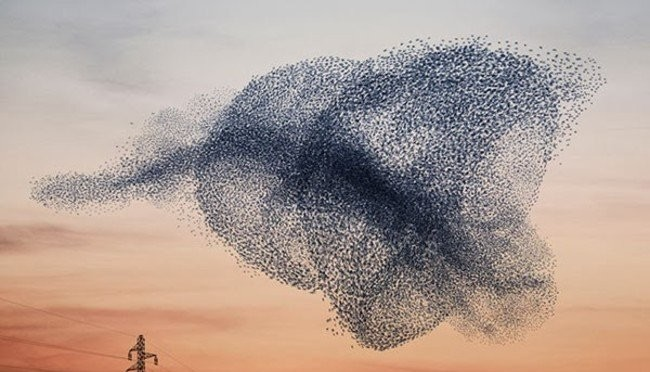
\includegraphics[width=0.8\linewidth]{images/Chapter1/Swarm birds.jpg}
        \caption{A flock of birds.}
        \label{fig:1.1}
    \end{minipage}%
    \begin{minipage}{.5\textwidth}
        \centering
        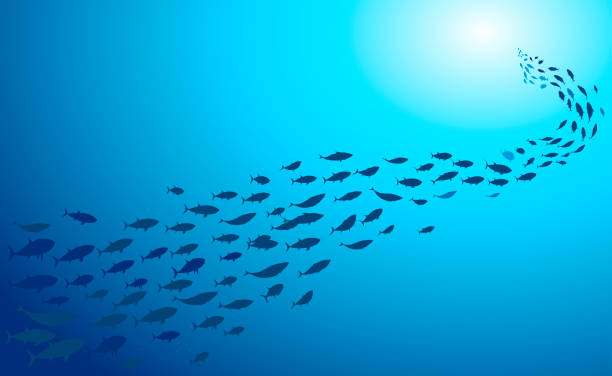
\includegraphics[width=0.8\linewidth]{images/Chapter1/Swarm fish.jpg}
        \caption{A swarm of fish.}
        \label{fig:1.2}
    \end{minipage}
        \begin{minipage}{.5\textwidth}
        \centering
        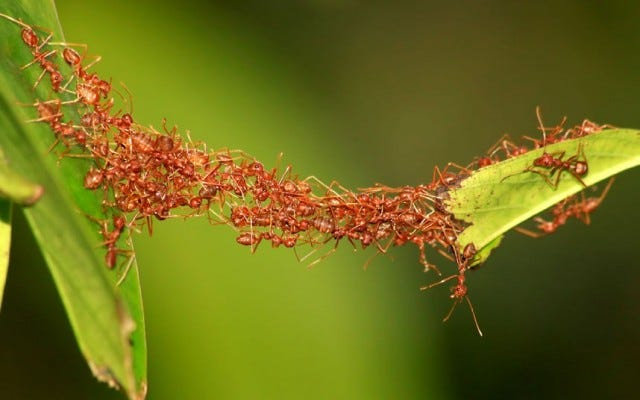
\includegraphics[width=0.8\linewidth]{images/Chapter1/Ant Swarm.jpg}
        \caption{A swarm of ants constructing a bridge.}
        \label{fig:1.3}
    \end{minipage}
\end{figure}

\newpage

A distributed system is a graph based architecture in which the nodes are the agents and the edges are the communication channels. Through the channels, each agent transmits and receives the data distributedly to his neighbor and vice versa. A representation of the architecture can be seen in figure \ref{fig:1.4}. A great application of the multi-agent systems is the consensus problem. According to the problem, the agents converge to a similar desired state, based on constraints of the information exchange between the agents of the network. According to \cite{1239709}, there have been developed a variety of consensus protocols. These protocols were developed in order to mimic the motion and the perception of swarms. So, the agents have a similar behavior to a swarm, thus achieving a desired goal, which was set, as a group.

\begin{figure}[H]
    \centering
    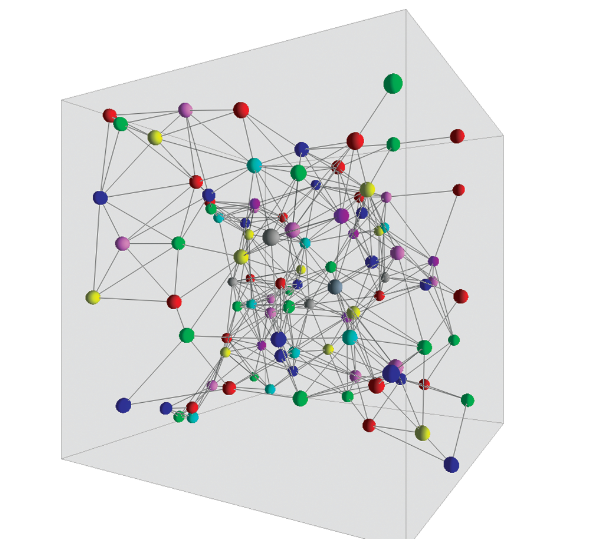
\includegraphics[width=0.3\linewidth]{images/Chapter1/Distributed network.png}
    \caption{Architecture of a distributed network.}
    \label{fig:1.4}
\end{figure}

In order to achieve consensus, the distributed system must receive specified commands. These commands are produced through a distributed control system. Such systems were designed in order to give specific tasks to agents for execution, \cite{DZW2021},\cite{LZHMD2014}. The field of distributed control attracted a significant number of scientists, leading to the development of novel control techniques. In addition, were developed two different approaches to the problem. The first method was centralized control, which is a master-slave approach. A master agent executes the task and exchanges local information with the other agents. The other agents follow the instructions given by the central agent. The second method of control is defined as decentralized or distributed. In this method, every agent acts based on local information which is available. The agents execute the desired tasks while exchanging information with their neighbors. Although, distributed control has a complex form, it is also a more realistic approach for appliance. As a result, physical systems have limitations, such as restricted range in communications, due to finite bandwidth and the number of the agents that exist in the network.

Recently, a number of issues have occurred regarding the distribution of the resources in various fields of applications, such as machine learning and automatic control. The answer to this problem comes from the area of distributed optimization. In particular, the optimal consensus problem is a reliable solution. The optimal consensus problem can be solved with cooperative control techniques and a distributed optimization problem. Therefore, every agent is equipped with a local cost function. Furthermore, agents are assigned to minimize the summation of these cost functions with respect to the constraints of the problem, while exchanging local information in intervals of time, \cite{DZW2021}.

The study of multi-agent systems led to the utilization of distributed optimization and distributed control techniques, in order to design robust methods. These results will not only lead to optimal solutions for current unsolved problems, but also for future ones.


\section{Motivation and Contribution}

The aim of this thesis is to solve the proximal optimal consensus problem, with non-convex constraints, for quadcopters who exchange partial information of their position with their neighbors, which are obtained at sampled periods of time. In addition, the algorithm will lead the agents in the region of the optimal point. In order to achieve this goal, NOn-Convex Gradient PROXimal (NOCGPROX) variables were defined, which are added into the Prox-GPDA algorithm, \cite{pmlr-v70-hong17a}, to prove the proximal optimal consensus. The development of robust distributed control laws that guarantee square integration of NOCGPROX variables is a crucial prerequisite for the convergence of the algorithm. In this manner, will be achieved proximal optimal consensus. Additionally, the quadcopters will be driven to the optimal consensus point. Furthermore, the signals of the closed loop system have to be bounded.

The thesis' contribution can be summarized in the following manner.

    \begin{itemize}
        \item  The NOCGPROX variables have been introduced, which transform the optimal consensus problem into a regulation one. This allows the problem to be solved with distributed control techniques, while achieving proximal optimal consensus, for agents with nonlinear dynamics.
        \item The proposed method for solving the problem depends on sampled filtered output measurements of the agents, thus achieving low frequencies in communication between them. Furthermore, it requires only the knowledge of the Laplacian matrix and the gradient of the local cost functions. In order to have stability in the system, it requires robust distributed control laws which ensures square integration of the variables. This improves the outline of the algorithm in cases in which the optimal solutions are not inside a feasible set.
        \item The design parameters of the algorithm must have large values to ensure sublinear stability of the method. In addition, NOCGPROX variables must tend to zero, to achieve optimal consensus.
    \end{itemize}


\section{Literature Review}

\subsection{Optimal Consensus Problem}
    A lot of scientific studies have been conducted in the years regarding distributed optimization. The foundation of distributed optimization was demonstrated in \cite{1104412}, in which a variety of asynchronous deterministic and stochastic methods have been developed with the use of gradient. From that point on, network systems have been designed and researched, putting into use distributed optimization algorithms for searching the best solution possible, either in discrete or continuous time.

    Regarding the application of distributed optimization in the consensus problem, most researchers have made use of discrete time algorithms in an attempt to reduce computational costs. The concept of the consensus problem has been studied throughout the years, with many scientific papers being published. An interest approach is presented in \cite{9162430}. The consensus between the agents is achieved through an adaptive schema which guarantee boundedness and regulation of the proposed variables with the sampled measurements being delayed. Additionally, in \cite{9785920} and \cite{9477076} is studied the optimal consensus problem. The optimal consensus is being achieved by utilizing a nonlinear PI controller, \cite{PSILLAKIS201911581}, which regulates the proposed variables with few transmissions of output measurements. In \cite{10125000} another solution is proposed, solving a proximal aspect of the optimal consensus problem. The solution is based on EXTRA algorithm for optimization, \cite{ShiEXTRA15}. The proposed variables ensure approximate consensus to a neighborhood of zero. 

\subsection{Convex and Non-Convex Optimization}
    There have been published numerous proposition for optimization algorithms in multi-agent systems. An algorithm whose being studied a lot is Alternating Direction Method of Multipliers (ADMM), \cite{10.1561/2200000016}. In \cite{9146334} has been proposed a different approach to the method. A more relaxed version is being developed which does not require synchronous updates between the agents with the constraints being convex, and achieve linear stability and convergence. On the other hand, in \cite{YANG2022110551} is proposed a proximal form of the algorithm for non-convex and nonsmooth functions. Non-convex problems are often more difficult to solve. On this proposed framework, these distributed optimization problems can be solved, thus achieving convergence.Another proposed methods for ADMM are presented in \cite{8704712} and \cite{wang2018global}. In both of these articles is presented two extension of the ADMM, which solve nonconvex and nonsmooth optimization, achieving global convergence of the state.

    In general, convex distributed optimization problems have been extensively studied and algorithms are currently have been developed, \cite{6358346},\cite{KIA2015254},\cite{10209260},\cite{DAI2020109256},\cite{SEMSARKAZEROONI20082766},\cite{GU20197548},\cite{QIU2016209}, \cite{8812749},\cite{FENG201612},\cite{YANG2018182},\cite{LIN2016120}, \cite{7500070},\cite{8899755},\cite{9316705},\cite{DOMINGUEZGARCIA201533}. While for nonconvex problems, there is a significant lack of solutions. Due to their structure, it is often difficult to find solutions. Fortunately, various methods have been developed in order to solve them. First, a proximate approach based on the primal-dual method is presented in \cite{pmlr-v70-hong17a}. The proposed approach is based on the primal-dual method, where the primal step minimizes a certain approximation of the augmented Lagrangian of the problem, and the dual step performs an approximate dual ascent, \cite{hong2016decomposing}. In addition, this proposed method transforms the nonconvex function into a strongly convex, thus creating a more linearized approach into solving the problem. The primal dual method is also used in \cite{LEI2016110}. Another primal-dual approach has been researched in \cite{7833143}. It is similar to \cite{pmlr-v70-hong17a}, but with different constraints and algorithm analysis. In \cite{7833143} is proposed an Accelerated Distributed Augmented Lagrangian method which has a faster convergent rate than a simple Augmented Lagrangian method. Another approach to solving nonconvex problems was studied by Paolo Di Lorenzo and Gesualdo Scutari in \cite{7398129},\cite{7383778},\cite{7869154}. A new method has been developed, named NEXT, which was the first algorithmic framework for distributed optimization of a sum of nonconvex (possibly and nonsmooth) cost functions. The described method uses a continuous convex approximation technique, which uses dynamic consensus to distribute computation among agents. Each agent first solves a local convex approximation of the non-convex problem (possibly inexactly) and then performs a local averaging operation. In \cite{7807315} was studied a general framework for nonconvex distributed optimization. To achieve convergence, a perturbed method was employed in the analysis, thus achieving optimal consensus among the agents. In \cite{8472181} and \cite{7776843}, two distributed techniques are being presented. In \cite{8472181} uses nonconvex constraints to bound the velocities of the agents with non-uniform position constrains. Based on a switching method is guaranteed boundedness of the state with sampled neighbor information. The same problem is solved in \cite{7776843}, with the only difference being the topology of the graph, which shifts overtime. Another research in nonconvex optimization is presented in \cite{9965620}. The objective is to steer the agents into an optimal point using partial information which is related to input and output. In addition, momentum-based optimal coordinators are design in order to achieve a steady-state. When solving an optimization problem, it is common for the solver to reach a local minimum. This problem is presented in \cite{9246278} with a solution for escaping local optima. The concept is to transform the gradient method into a boosted gradient with nonzero magnitude. Thus, the  optimizer will converge into a global minimum. In \cite{10025380,9462469} is presented a nonconvex framework for solving online the optimization problem using dynamic regrets. In this proposed framework, \cite{FARINA2019243}, is presented an asynchronous distributed approach in which both objective function and constraints are nonconvex. It uses a trigger event on which every node has limited access to the function and the constraints. During that time, the method of multipliers is applied to minimize the Augmented Lagrangian. 

    Most optimization algorithms use gradients to be solved. However, there exists a number of algorithms who are gradient free. These algorithms from their nature are stochastic. An interesting research was conducted by Hajinezhad and Zavlanos in \cite{8619333}, where the distributed nonconvex optimization is being solved without the use of gradient. Their approach is based on a primal dual method, in which every agent has access only to partial information about the global cost function, knowing only the zeroth-order information of their local cost function.

\subsection{Graph Topology Variations}
    While the objective function fulfills a significant role in distributed optimization of the agents, there is another factor that contributes towards the problem. It is also important to consider the topology of the graph. Most of the above mention researches have an undirected topology considering the graph. In \cite{GU20197548}, \cite{DOMINGUEZGARCIA201533}, \cite{9112274}, \cite{6894574}, \cite{9992866} and \cite{YOO2018421} the topology of the graph is directed. The main categorization of the topology lies into static and dynamic graphs. The static graphs have one topology that does not change in time. While dynamic topology (or switching topology) changes in time. Therefore, the matrices and vectors of the problem are time variant. In fact, it's clear from \cite{8340193} that different ways of solving the optimization problem exist, regarding the topology. Throughout the graph is observed the communication tradeoff of the agents. Thus, network topology fulfills a crucial role in the analysis. 

    Although fixed topologies have been extensively studied throughout the years, research has been conducted on switching topologies as well. A thoroughly established illustration of the usage of both fixed and switching topology is studied in \cite{8723151}. A class of distributed nonlinear controllers have been designed in order to achieve consensus for high-order agents in both topologies. In \cite{8445642} a similar approach is presented, but with unknown high frequency gain signs. The method which was proposed assures consensus between the agents with non-identical unknown control directions under the switching graph. A more probabilistic approach is presented in \cite{5404835}. While exchanging packages, the agents change their topology randomly when a packet is lost. As a result, the agents are modelled as a system with a stochastic switching undirected topology, which in conjunction with the proposed algorithm is robust to ensure consensus. Oftentimes, consensus protocols tend to be executed asynchronous between the agents. Such cases are presented in \cite{9244621} and \cite{4631522}. In the first one, a switched observer was designed which estimates the state information of the leader, which is based on a general switching topology rule of the spanning tree of the graph. While feedback distributed control laws ensure consensus in all modes of the graph. The later one, ensures consensus between the agents, while the topology switches during time-delays. In \cite{9736623} is presented a novel approach regarding the losses which occurs during the switching of the topology. This simple approach is base on a high-order filter to generate differentiable control variables using neighbor position information  and discontinuous topology information. Another research paper is presented in \cite{6839031}, which ensures robust consensus tracking control, considering the fact that the topology changes in time with disturbances in the communications. Lastly, in \cite{8100757} is presented an adaptive mechanism which ensures cooperation between the agents under switched topologies. In this paper are presented two distributed event-trigger control schemes, in which the agents track reference inputs asymptotically and reject disturbances. 

\section{Thesis Structure}

This diploma thesis consists of six chapters in total. The first chapter contains the introduction for this thesis and the motivation behind it. In addition, the chapter also contains the review of the literature. The chapter also contains the thesis structure and bibliography.

The second chapter discusses the fundamental mathematical concepts and axioms utilized for proving and designing both the algorithm and the robust distributed control laws.

In the third chapter, the NOCGPROX variables are introduced in order to solve the proximal output consensus. Additionally, it contains a mathematical proof analysis of the algorithm with its lemmas and theorem, which prove proximal consensus.

In the fourth chapter, the nonlinear dynamics of the agents are transformed to incorporate the NOCGPROX variables into the dynamics. The robust distributed control laws are introduced which ensure the square integration of the variables with sliding surface feedback linearization method to ensure that the variables tends to zero and be square integrable.

The fifth chapter is consisted of the simulation of the algorithm and control laws for the agents. In the simulation, there are applied different scenarios in order to achieve optimal consensus of the agents.

The sixth and final chapter contains the concluding remarks of this thesis and purpose, while future research is discussed for improvements of this work.
    
%--------------------------------------------------------------------
    \chapter{Mathematical Background}
    
In this chapter, the mathematical background of this thesis is presented. Specifically, is introduced the basic notations and definitions of graph theory, as well some mathematical concepts of matrix theory, Lyapunov stability theory and basic theorems of mathematical analysis. In addition, is introduced and the augmented Lagrangian algorithm.

\section{Graph Theory}

\subsection{Basic Definitions}
    \begin{definition}\label{def:2.1}
        \cite{GR2001} A finite graph $\mathcal{G}$ is a non-empty finite set $\mathcal{G} = (\mathcal{V},\mathcal{E},\mathcal{A})$ which is consisted of a finite non-empty set $\mathcal{V}(\mathcal{G})$, a finite non-empty set $\mathcal{E}(\mathcal{G})$ and $\mathcal{A}$ is the incidence matrix of the graph. The set $\mathcal{V}(\mathcal{G})$ contains the vertices (nodes) of the graph, with $|\mathcal{V}| = N$ and the set $\mathcal{E}(\mathcal{G})$ contains the edges of the graph with $|\mathcal{E}| = E$, which connect the vertices. 
    
        If there exists an edge between the vertices $v_i$ and $v_j$, then the vertices are defined as adjacent with the symbol $v_i \sim v_j$.
        \begin{figure}[H]
            \centering
            \begin{minipage}{.5\textwidth}
                \centering
                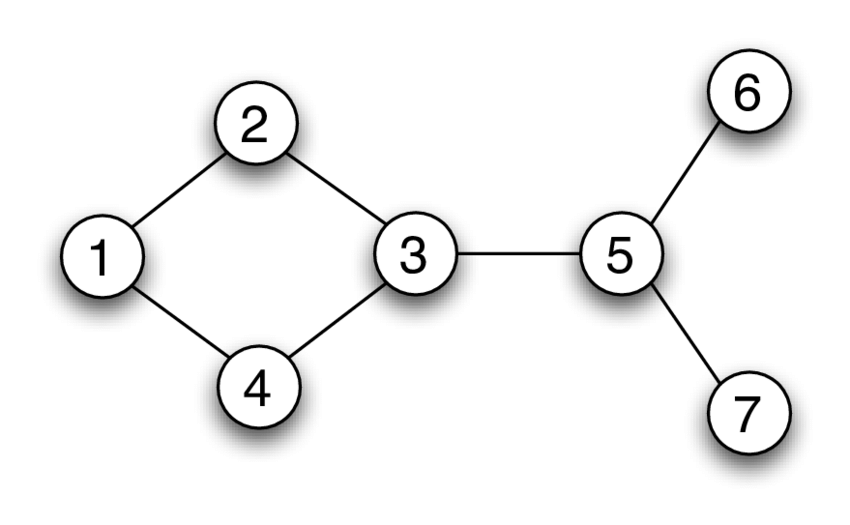
\includegraphics[width=0.8\linewidth]{images/Chapter2/undigraph.png}
                \caption{Undirected graph topology.}
                \label{fig:2.1}
            \end{minipage}%
            \begin{minipage}{.5\textwidth}
                \centering
                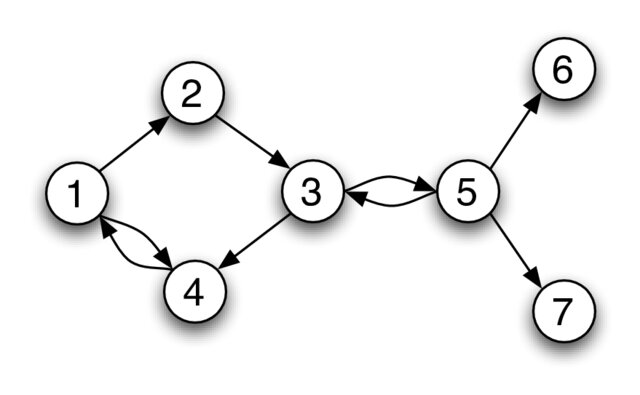
\includegraphics[width=0.8\linewidth]{images/Chapter2/digraph.png}
                \caption{Directed graph topology.}
                \label{fig:2.2}
            \end{minipage}
        \end{figure}
    \end{definition}
    \newpage
     \begin{definition}\label{def:2.2}
         \cite{GR2001} A neighborhood of an $i-$agent is defined as\\ $\mathcal{N}(i) := \left\{ j \in \mathcal{V} \hspace{0.5mm} | \hspace{0.5mm}  (i,j) \in \mathcal{E}\right\} \subset \mathcal{V}$.
     \end{definition}
    
    \begin{definition}\label{def:2.3}
        \cite{GR2001} A path of length $l$ from $\{v_{i_0}, v_{i_1}, ..., v_{i_l}\}$ in a graph is a sequence of $l + 1 $ distinct nodes starting with $v_{i_0}$ and ending with $v_{i_l}$ such that consecutive nodes are adjacent.
    \end{definition}
    
     \begin{definition}\label{def:2.4}
         \cite{GR2001} A cycle is a connected graph where every node has exactly two neighbors.
     \end{definition}
    \begin{definition}\label{def:2.5}
        \cite{GR2001} A graph $\mathcal{G}$ is connected, if for every pair of nodes of $\mathcal{V}(G)$, exists a path which have this pair as an end.
    \end{definition}
    
     \begin{definition}\label{def:2.6}
         \cite{GR2001} If in a graph, in addition to its nodes and edges, exists a function $\mathcal{W}:E \to \mathbf{R}$ where assigns a value in every edge, then the graph $\mathcal{G} = (\mathcal{V}, \mathcal{E}, \mathcal{W})$ is called weighted graph.
        \begin{figure}[H]
            \centering
            \begin{minipage}{.5\textwidth}
                \centering
                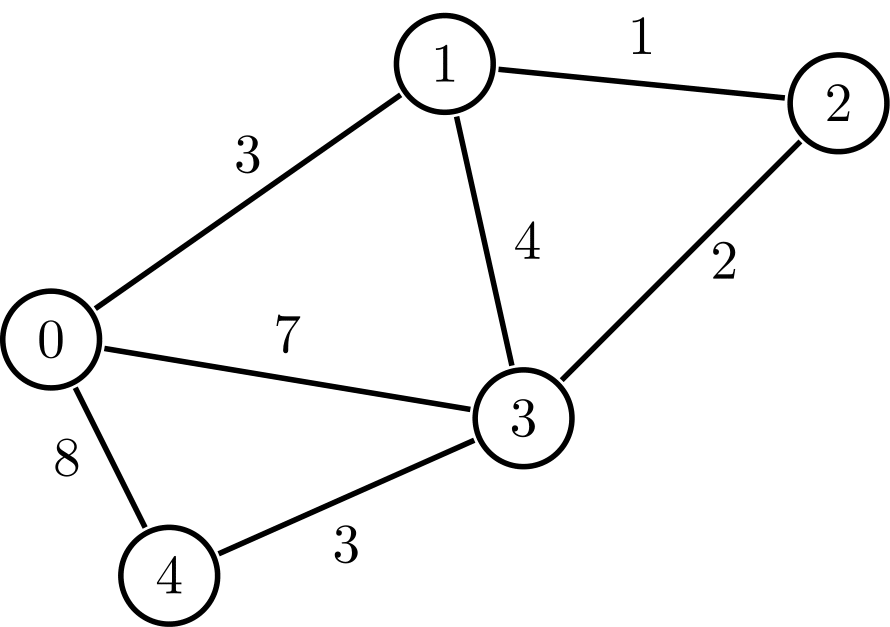
\includegraphics[width=0.8\linewidth]{images/Chapter2/weight graph.png}
                \caption{Undirected weighted \\graph topology.}
                \label{fig:2.3}
            \end{minipage}%
            \begin{minipage}{.5\textwidth}
                \centering
                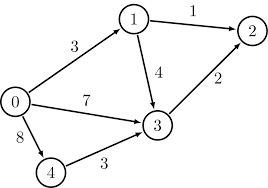
\includegraphics[width=0.8\linewidth]{images/Chapter2/weight digraph.png}
                \caption{Directed weighted \\graph topology.}
                \label{fig:2.4}
            \end{minipage}
        \end{figure}
     \end{definition}
    
\subsection{Graph Matrices}

    In addition to the basic graph notations, matrices can describe them in an algebraic form. Due to the selected algorithm, an incidence matrix is used.
    
    \begin{definition}\label{def:2.7}
        \cite{GR2001} The degree $d(v_i)$ of a node in an undirected graph $\mathcal{G}$ is the total number of nodes which are adjacent to $v_i$.
    \end{definition}
    
    \begin{definition}\label{def:2.8}
        \cite{GR2001} The degree matrix $D$ of an undirected graph $\mathcal{G}$ is a diagonal matrix whose elements are the degree nodes $d(v_i)$. 
    \end{definition}
    
    
    \begin{definition} \label{def:2.9}
        \cite{hong2016decomposing} The incidence matrix $\mathcal{A}$ is a $N \times E$ matrix, which describes the relationship between a node and an edge. In its $i-$th row and $j-$th column has the number of times the $j-$th edge is incident with the $i-$th vertex. Now the matrix is defined as
        
        \begin{equation}\label{eq:2.1.1}
            [\mathcal{A}]_{ev} = \left\{ \begin{matrix}
                1,\hspace{5.0mm} if \hspace{2.0mm}(i,j) \in \mathcal{E}, with \hspace{2.0mm} i > j \hspace{2.0mm} and \hspace{2.0mm} v = i \\
                -1,\hspace{5.0mm} if \hspace{2.0mm}(i,j) \in \mathcal{E}, with \hspace{2.0mm} i > j \hspace{2.0mm} and \hspace{2.0mm} v = j \\
                0,\hspace{20.0mm} otherwise \end{matrix} \right
        \end{equation}
        
    \end{definition}
    
    
    \begin{definition}\label{def:2.10}
        \cite{GR2001} The Laplacian matrix of an undirected graph $\mathcal{G}$ is defined by
        \begin{equation}\label{eq:2.1.2}
            L= D - \mathcal{A}
        \end{equation}
        where $D$ is the degree matrix and $\mathcal{A}$ is the incidence matrix.
    \end{definition}
    
    \begin{definition}\label{def:2.11}
        \cite{hong2016decomposing} The signed Laplacian matrix of a graph $\mathcal{G}$ is defined as
        \begin{equation}\label{eq:2.1.3}
            L_- = \mathcal{A}^T\mathcal{A}
        \end{equation}
    \end{definition}
    
    \begin{definition}\label{def:2.12}
        \cite{hong2016decomposing} The signless Laplacian matrix of a graph $\mathcal{G}$ is defined as
        \begin{equation}\label{eq:2.1.4}
            L_+ = 2D - \mathcal{A}^T\mathcal{A}
        \end{equation}
    \end{definition}
    

\section{Matrix Theory}

    In this section are going to be introduced the basic notations of matrix theory that will be used.
    
    \begin{definition}\label{def:2.13}
        \cite{strang2006linear} Consider a vector field of $\mathbf{R}^n$ and a squared matrix $A \in \mathbf{R}^{n \times n}$. Then, for a vector $x \in \mathbf{R}^n$ and a constant $\lambda \in \mathcal{C}$ holds that
    
        \begin{equation}\label{eq:2.2.1}
            Ax = \lambda x
        \end{equation}
        where $x$ is called eigenvector of matrix $A$ which is related to the eigenvalue $\lambda$.
    \end{definition}
    The matrix $A$ can be inverted, if he does not have a zero eigenvector. The eigenvalues of a matrix are computed from
    
    \begin{equation}\label{eq:2.2.2}
        \chi_A(\lambda) = det(\lambda I_n - A) = 0
    \end{equation}
    This equation is called the characteristic polynomial of the matrix $A$, with the eigenvalues being its roots. The algebraic multiplicity of an eigenvalue $\lambda$ is the multiplicity as a root of the equation (\ref{eq:2.2.2}). The geometric multiplicity of an eigenvalue $\lambda$, is the maximum number of linear independent eigenvectors, which are associated with this eigenvalue.
    
    \begin{theorem}\label{thr:2.1}
        \cite{strang2006linear}  Let $S$ be a matrix of eigenvectors of a given square matrix $A$ and $\Lambda$ be a diagonal matrix with the corresponding eigenvalues on the diagonal. Then, as long as $S$ is a square matrix, matrix $A$ can be written as an eigen decomposition
        \begin{equation}\label{eq:2.2.3}
            A = S\Lambda S^{-1}
        \end{equation}
        where $\Lambda$ is a diagonal matrix. Furthermore, if $A$ is symmetric, then the columns of $S$ are orthogonal vectors. 
    \end{theorem}
    
    \begin{definition}\label{def:2.14}
        \cite{strang2006linear} A matrix $A$ is called semipositive if the quadratic form
        \begin{equation*}
            x^TAx \geq 0, \forall x
        \end{equation*}
        and positive if the quadratic form is
        \begin{equation*}
            x^TAx > 0, \forall \hspace{2.0mm} x  \neq 0
        \end{equation*}
    \end{definition}
    
    \begin{corollary}\label{cor:2.1}
        \cite{strang2006linear} A matrix $A$ is semipositive iff all his eigenvalues are nonnegative. A matrix $A$ is positive if all his eigenvalues are positive.
    \end{corollary}
    
    \begin{definition}\label{def:2.15}
        \cite{strang2006linear} A matrix $ A \in \mathbf{R}^{n\times n}$ is defined as nonnegative if his elements are nonnegative, i.e. $\alpha_{ij} \geq 0$, for $i,j = 1,...,n$.
    \end{definition}
    
    \begin{definition}\label{def:2.16}
        \cite{strang2006linear} The Kronecker product of two matrices $A \in \mathbf{R}^{n\times m}$ and $B \in \mathbf{R}^{p \times q}$, with $\alpha_{ij} = [A]_{ij}$ and $b_{ij} = [B]_{ij}$, is written as $A \otimes B$ and defined as an $np \times mq$ matrix below
    
        \begin{equation} \label{eq:2.2.4}
            A \otimes B = \left[\begin{matrix}
                 \alpha_{11}B & \cdots & \alpha_{1m}B \\
                    \alpha_{21}B & \cdots & \alpha_{2m}B \\
                    \vdots & \vdots & \vdots \\
                    \alpha_{n1}B & \cdots & \alpha_{nm}B
            \end{matrix} \right]
        \end{equation}
    \end{definition}
    The properties of the Kronecker product are presented below
    
    \begin{equation*}
            A \otimes (B + C) = A \otimes B + A \otimes C
    \end{equation*}
    \begin{equation*}
        (kA) \otimes B = A \otimes (kB) = k(A \otimes B)
    \end{equation*}
    \begin{equation*}
        (A \otimes B) \otimes C = A \otimes (B \otimes C)
    \end{equation*}
    \begin{equation*}
         A \otimes 0 = 0 \otimes A = 0
    \end{equation*}
    where matrices $A,B,C$ have the appropriate dimensions, $0$ is the zero matrix and $k$ is constant.
    

\section{Mathematical Analysis}
    
    In this section are presented the basic notations, theorems and definitions of mathematical analysis. Specifically of real analysis, functional analysis and convex and non-Convex analysis.
    \begin{definition}\label{def:2.17}
        \cite{folland2013real} A continuous function $a:\mathbf{R}_+ \to [0,\infty)$ is a class $\mathcal{K}$ \\function if
        \begin{itemize}
            \item $a \in C^0(\mathbf{R}_+)$
            \item it is strictly increasing in $\mathbf{R}_+$
            \item $a(0) = 0$
        \end{itemize}
    \end{definition}
    \begin{definition}\label{def:2.18}
        \cite{folland2013real} A continuous function $a:\mathbf{R}_+ \to [0,\infty)$ is a class $\mathcal{K}_{\infty}$ \\function if
        \begin{itemize}
            \item $a \in C^0(\mathbf{R}_+)$
            \item it is strictly increasing in $\mathbf{R}_+$
            \item $a(0) = 0$
            \item $\lim_{s \to \infty} a(s) = \infty$
        \end{itemize}
    \end{definition}
    \begin{definition}\label{def:2.19}
        \cite{folland2013real} A continuous function $a: \mathbf{R_+} \times \mathbf{R_+} \to \mathbf{R_+}$ is a class $\mathcal{KL}$ function if
        \begin{itemize}
            \item $a(\cdot, t)$ is strictly increasing in $\mathbf{R_+}$, $\forall t \geq 0$
            \item $a(s,\cdot)$ is strictly decreasing in $\mathbf{R_+}$, $\forall s \leq 0$
            \item $\lim_{t \to \infty} a(s,t) = 0, \forall s \geq 0$
            \item $a(0,t) = 0, \forall t \geq 0$
        \end{itemize}
    \end{definition}
    
    \begin{definition}\label{def:2.20}
        \cite{HK2001} A continuous function $W: \mathbf{R}^n \to \mathbf{R}$ is positive defined iff
        \begin{itemize}
            \item $W(0) = 0$
            \item $W(x) > 0$, \hspace{2.0mm} $\forall x \in \mathbf{R}^n - \{0\}$
            \item exists $r > 0$, such that $\inf_{||x|| \geq r} W(x) > 0$
        \end{itemize}
    \end{definition}
    
    \begin{definition}\label{def:2.21}
        \cite{HK2001} Young inequality is defined as
        \begin{equation}\label{eq:2.3.1}
            a \cdot b \leq \frac{\epsilon}{2}a^2 + \frac{1}{2\epsilon}b^2, \forall a,b \in \mathbf{R}, \forall \epsilon > 0
        \end{equation}
    \end{definition}
    
    \begin{definition}\label{def:2.22}
        \cite{folland2013real} Assume that $p$ and $q$ are in the open interval $(1,\infty)$ with $1/p + 1/q = 1$. Hölder's inequality is defined as
        \begin{equation}\label{eq:2.3.2}
            \left(\sum_{i = 1}^{n} |a_i b_i|\right) \leq \left(\sum_{i = 1}^{n} |a_i|^p\right)^{1/p} \left(\sum_{i = 1}^{n} |b_i|^q\right)^{1/q} 
        \end{equation}
        if $|a_i| = 1$ then
        \begin{equation*}
            \left(\sum_{i = 1}^{n} |a_i b_i|\right) \leq \left(\sum_{i = 1}^{n} |a_i|^p\right)^{1/p} \left(\sum_{i = 1}^{n} |b_i|^q\right)^{1/q}\leq n^{1-p}\left(\sum_{i = 1}^{n} |b_i|^p\right)
        \end{equation*}
    \end{definition}
    
    \begin{definition}\label{def:2.23}
        \cite{JBI1991} A function $f \in C^1({\mathbf{R}^n})$ is called $L-$smooth if satisfies the below inequality, \hspace{1.0mm}$\forall x_1,x_2 \in \mathbf{R}^n$:
        \begin{equation}\label{eq:2.3.3}
            ||\nabla f(x_1) -\nabla f(x_2)|| \leq L ||x_1 - x_2||
        \end{equation}
        or
        \begin{equation}\label{eq:2.3.4}
            |f(x_1) - f(x_2) - \nabla f(x_2)^T(x_1 - x_2)| \leq \frac{L}{2}||x_1 - x_2||^2
        \end{equation}
    \end{definition}
    
    \begin{definition}\label{def:2.24}
        \cite{JBI1991} A function $f \in C^1({\mathbf{R}^n})$ is called convex, if \hspace{1.0mm}$\forall x_1,x_2 \in \mathbf{R}^n$:
        \begin{equation}\label{eq:2.3.5}
            f(x_1) - f(x_2) \geq f(x_2)^T(x_1 - x_2) 
        \end{equation}
    \end{definition}
    
    \begin{definition}\label{def:2.25}
        \cite{JBI1991} A function $f \in C^1({\mathbf{R}^n})$ is called $\sigma-$strongly convex, with $\sigma > 0$, if \hspace{1.0mm}$\forall x_1,x_2 \in \mathbf{R}^n$:
        \begin{equation}\label{eq:2.3.6}
            f(x_1) - f(x_2) - f(x_2)^T(x_1 - x_2) \geq \frac{\sigma}{2}||x_1 - x_2||^2
        \end{equation}
        if $f \in C^2({\mathbf{R}^n})$, is strongly convex and smooth then
        \begin{equation}\label{eq:2.3.7}
            \sigma I_n \preceq \nabla^2 f(x) \preceq LI_n
        \end{equation}
        where $I_n \in \mathbf{R}^{n \times n}$ is the unit matrix with size $n$. If $f(x_1) - f(x_2) - f(x_2)^T(x_1 - x_2) \geq 0$, then from (\ref{eq:2.3.4}) and (\ref{eq:2.3.6}) is obtained:
        \begin{equation}\label{eq:2.3.8}
            \frac{\sigma}{2}||x_1 - x_2||^2 \leq f(x_1) - f(x_2) - f(x_2)^T(x_1 - x_2) \leq \frac{L}{2}||x_1 - x_2||^2
        \end{equation}
    \end{definition}
    
    \begin{definition}\label{def:2.26}
        \cite{JBI1991} A function $f \in C^1({\mathbf{R}^n})$ is called Lipschitz, if  \hspace{1.0mm}$\forall x_1,x_2 \in \mathbf{R}^n$ and a constant $\mathbf{L} \geq 0$:
        \begin{equation}\label{eq:2.3.9}
            ||f(x_1) - f(x_2)|| \leq \mathbf{L} ||x_1 - x_2||
        \end{equation}
    \end{definition}
        
    \begin{definition}\label{def:2.27}
        \cite{JBI1991} A function $f(x)$ is called locally Lipschitz in $\mathcal{D} \subset \mathbf{R}^n$, if every point of $\mathbf{D}$ has an area $\mathbf{D}_0$ which satisfies the Lipschitz condition for a Lipschitz constant $\mathbf{L}_0$. 
    \end{definition}
    
    \begin{definition}\label{def:2.28} 
        \cite{JBI1991} A function $f(x)$ is called globally Lipschitz if it is Lipschitz on $\mathbf{R}^n$.
    \end{definition}
    
    \begin{theorem}\label{thr:2.2}
        \cite{ZSCSP} If $f:R^n \to  R$ is a Lipschitz continuously differentiable on a convex set $\mathcal{C}$\hspace{1.0mm} ($f \in C^1(\mathcal{C})$) with some Lipschitz constant $\mathbf{L}$, then $\phi(x) = f(x) - \frac{1}{2}ax^Tx$ is a convex function on $\mathcal{C}$ for every $a \leq -\mathbf{L}$.
    \end{theorem}

\section{Lyapunov Stability Theory}

    Lyapunov theory was invented from the Russian mathematician Aleksandr Lyapunov, in order to study the stability of dynamical systems. Through his findings, he was able to conclude if a dynamical system is either stable or unstable. The basic concept of stability theory is the definition of a suitable scalar function, which is analyzed to evaluate its properties.

    Consider the $n-$dimensional system

    \begin{equation}\label{eq:2.4.1}
        \dot{\boldsymbol{x}} = f(\boldsymbol{x})
    \end{equation}
    where $f: \mathcal{D} \to \mathbf{R}^n$ is locally Lipschitz over a domain $\mathcal{D} \subset \mathbf{R}^n$. Suppose $\boldsymbol{x}^*$ is an equilibrium point of (\ref{eq:2.4.1}); that is $f(\boldsymbol{x}^*) = 0$.

    \begin{definition}\label{def:2.29}
        \cite{HK2001} Let $f(x)$ be a locally Lipschitz defined over a domain $\mathcal{D} \subset \mathbf{R}^n$, which contains the origin, and $f(0) = 0$. The equilibrium point $x^* = 0$ 0f (\ref{eq:2.4.1}) is
        \begin{itemize}
            \item stable if for each $\varepsilon > 0$ there is $\delta > 0$ (dependent on $\varepsilon$) such that
                \begin{equation*}
                    ||x(0)|| < \delta \Rightarrow  ||x(t)|| < \varepsilon, \forall t \geq 0
                \end{equation*}
            \item unstable if it is not stable.
            \item asymptotically stable if it is stable and $\delta$ can be chosen such that
                \begin{equation*}
                    ||x(0)|| < \delta \Rightarrow \lim_{t \to \infty} x(t) = 0
                \end{equation*}
            \item exponentially stable if there exists $\delta, M, \sigma$ such that
            \begin{equation*}
                ||x(0)|| < \delta \Rightarrow ||x(t)|| \leq Me^{-\sigma t}||x(0)||, \hspace{1.0mm} \forall t \geq 0
            \end{equation*}
        \end{itemize}
    \end{definition}
    

    \begin{definition}\label{def:2.30}
        \cite{HK2001} Consider a function $V: \mathbf{R}^n \to R$, which:
        \begin{itemize}
            \item $V(0) = 0$
            \item $V(x) > 0$, $\forall x \neq 0$
        \end{itemize}
        then it is a positive define function. This function is called Candidate Lyapunov function.
    \end{definition}

    \begin{definition}\label{def:2.31}
        \cite{HK2001} A Lyapunov function $V: \mathbf{R}^n \to R$ is called radially unbounded, if $\forall M > 0$ the set $\{x\in\mathbf{R}^n: \hspace{2.0mm} V(x) \leq M\}$ is bounded, or
        \begin{equation*}
            \lim_{||x|| \to +\infty} V(x) = +\infty
        \end{equation*}
    \end{definition}

    \begin{theorem}\label{thr:2.4}
        \cite{HK2001} Consider a positive defined function $V \in C^1(\mathbf{R}^n)$. Consider an open set $\mathcal{D} \subset \mathbf{R}^n$, with the $0$ inside it such that
        \begin{equation*}
            \nabla V(x) f(x)\leq 0, \forall x \in \mathcal{D}
        \end{equation*}
        then, $0 \in \mathbf{R}^n$ is stable for the system of (\ref{eq:2.4.1}).
    \end{theorem}
    
    
    \begin{theorem}\label{thr:2.5}
        \cite{HK2001} Consider a positive defined function $V \in C^1(\mathbf{R}^n)$. Consider an open set $\mathcal{D} \subset \mathbf{R}^n$, with the $0$ inside it such that
        \begin{equation*}
            \nabla V(x) f(x) < 0, \forall x \in \mathcal{D}, \forall x \neq 0
        \end{equation*}
        then, $0 \in \mathbf{R}^n$ is asymptotically stable for the system of (\ref{eq:2.4.1}).
    \end{theorem}
    
    \begin{definition}\label{def:2.32}
        \cite{HK2001} The equilibrium point of (\ref{eq:2.4.1}) is
        \begin{itemize}
            \item uniformly bounded if there exists a positive constant $c$, independent of $t_0 \geq 0$, and for every $a \in (0,c)$, there exists $\beta = \beta(a) > 0$, independent of $t_0$, such that
            \begin{equation}\label{eq:2.4.2}
                ||x(t_0)|| \leq 0 \Rightarrow ||x(t)|| \leq \beta, \forall t \geq t_0
            \end{equation}
            \item globally uniformly bounded if (\ref{eq:2.4.2}) holds for arbitrarily large $a$.
            \item uniformly ultimately bounded with ultimate bound $b$ if there exists positive constants $b$ and $c$, independent of $t_0 \geq 0$, and for every $a \in (0,c)$, there is $T = T(a,b) \geq 0$, independent of $t_0$, such that
            \begin{equation}\label{eq:2.4.3}
                ||x(t_0)|| \leq a \Rightarrow ||x(t)|| \leq b, \forall t \geq t_0 + T
            \end{equation}
            \item globally uniformly ultimately bounded if (\ref{eq:2.4.3}) holds for arbitrarily large $a$.
        \end{itemize}
    \end{definition}
    

    \begin{lemma}\label{lem:2.1}
        \cite{HK2001} Let $V: \mathcal{D} \to \mathbf{R}$ be a continuous positive function defined inside the domain $\mathcal{D} \subset \mathbf{R}^n$ that contains the origin. Let $B_r \subset \mathcal{D}$ for some $r > 0$. Then, there exist class $\mathcal{K}$ functions $a_1$ and $a_2$, defined on $[0,r]$, such that
        \begin{equation}\label{eq:2.4.4}
            a_1(||x||) \leq V(x) \leq a_2(||x||)
        \end{equation}
        $\forall x \in B_r$. If $\mathcal{D} = \mathbf{R}^n$, the functions $a_1$ and $a_2$ will be defined on $[0, \infty)$ and the foregoing inequality will hold $\forall x \in \mathbf{R}^n$. Moreover, if $V(x)$ is radially unbounded, then $a_1$ and $a_2$ can be chosen to belong to class $\mathcal{K}_{\infty}$.
    \end{lemma}
        

\section{Augmented Lagrangian Algorithm}

Augmented Lagrangian Algorithms have a primal dual multiplier form, \cite{bertsekas2015incremental}, which minimize the summation of the cost function with respect to the constraints of the problem. The algorithm which will be used in this dissertion is Prox-GPDA, \cite{pmlr-v70-hong17a,hong2016decomposing}, which is a proximal form of the classic augmented Lagrangian algorithm with an added proximal term. Consider the following optimization problem

\begin{equation}\label{eq:2.5.1}
    \min_{x \in \mathbf{R}^n} g(x) = \sum_{i = 1}^{N} f_i(x)
\end{equation}
where $f_i(x):\mathbf{R}^n \to \mathbf{R}$, $i\in \{1,...,N\}:= [N]$ are the nonconvex local cost functions of each agent, which are assumed to be smooth and has Lipschitz continuous gradients. Suppose the agents are connected with an undirected graph which is defined in \ref{def:2.1}. Each agent can only exchange information with his neighbor, defined as in \ref{def:2.2} with $|\mathcal{N}_i| = d_i$. The distributed version of problem (\ref{eq:2.5.1}) is

\begin{equation}\label{eq:2.5.2}
    \min_{x_i \in \mathbf{R}^n} f(x) := \sum_{i = 1}^{N} f_i(x_i),\hspace{1.0mm} s.t.\hspace{1.0mm} x_i = x_j,\hspace{1.0mm} \forall (i,j) \in \mathcal{E}
\end{equation}

It is clearly that the problem (\ref{eq:2.5.2}) is equivalent to the problem (\ref{eq:2.5.1}) as long as the graph $\mathcal{G}$ is connected. For notational simplicity, the sequence $x:=\{x_i\} \in \mathbf{R}^{Nn \times 1}$, and $Q = N \times n$. The incidence matrix is introduced in \ref{def:2.9}. In order for the dimensions to be matched, we defined the extended incidence matrix as

\begin{equation}\label{eq:2.5.3}
    A = \mathcal{A} \otimes I_n \in \mathbf{R}^{En \times Q}
\end{equation}
In the same manner, the degree matrix is defined as
\begin{equation}\label{eq:2.5.4}
    \mathbf{D} = D \otimes I_n \in \mathbf{R}^{Q \times Q}
\end{equation}
Lastly, the Laplacian matrices are defined in \ref{def:2.11} and \ref{def:2.12}. The extended form of the signed and the signless Laplacian are:
\begin{equation}\label{eq:2.5.5}
    L_{-} = L_{-} \otimes I_n \in \mathbf{R}^{Q \times Q}, \hspace{2.0mm}\\
    L_{+} = L_{+} \otimes I_n \in \mathbf{R}^{Q \times Q}
\end{equation}
Using the notations above, the problem \ref{eq:2.5.2} can be rewritten in the following compact form
\begin{equation}\label{eq:2.5.6}
    \min_{x \in \mathbf{R}^Q} f(x), \hspace{2.0mm} s.t. \hspace{1.0mm}Ax = 0
\end{equation}
\newpage
Prox-GPDA is built upon the classical Augmented Lagrangian Method,\cite{bertsekas2015incremental}. It is defined as

\begin{equation}\label{eq:2.5.7}
    L_{\beta}(x,\mu) = f(x) + \langle \mu, Ax\rangle + \frac{\beta}{2} ||Ax||^2
\end{equation}
where $\mu \in \mathbf{R}^Q$ is the Lagrangian dual variable; $\beta > 0$ is a penalty parameter. Let the matrix $B \in \mathbf{R}^{Q\times Q}$ which is some arbitrary matrix that will be defined in the analysis. The proposed algorithm Prox-GPDA is shown below,\cite{hong2016decomposing}.

\begin{algorithm}[H]
    \caption{The Proximal Gradient Primal Dual Algorithm (Prox-GPDA)}\label{alg:prox-gpda}
    \textbf{Input}: $\mu^0 = 0$, $x^0 \in \mathbf{R}^Q$\\
    \textbf{Output}: $x^{r+1} \in \mathbf{R}^Q$
    \begin{algorithmic}[1]
        \begin{flushleft}
            At each iteration $r+1$, update variables by:
        \end{flushleft}
        \begin{subequations}\label{eq:2.5.8}
            \begin{gather}
                x^{r+1} = arg \min_{x \in \mathbf{R}^Q} \langle \nabla f(x^r), x - x^r\rangle + \langle \mu^r, Ax\rangle + \frac{\beta}{2} ||Ax||^2 + \frac{\beta}{2}||x - x^r||^2_{B^TB}\label{eq:2.5.8a}\\
                \mu^{r+1} = \mu^r + \beta A x^{r+1}\label{eq:2.5.8b}
            \end{gather}
        \end{subequations}
    \end{algorithmic}
\end{algorithm}

As seen in algorithm \ref{alg:prox-gpda}, the cost function has been replaced with a proximal gradient step, in order to solve $x-$subproblem (\ref{eq:2.5.8a}). This is efficient, hence does not require computations of the zeroth order of the function $f(x)$. It is also advantageous in cases where the cost function is not available. Furthermore, the proximal term which is introduced in the algorithm is $\frac{\beta}{2}||x - x^r||^2_{B^TB}$. This term is crucial in both the algorithm implementation and analysis, hence it ensures
\begin{enumerate}
    \item The primal problem transforms form nonconvex in strongly convex.
    \item The primal problem is decomposable over different network nodes, thus distributedly implementable.
\end{enumerate}
In order to ensure these properties, the matrix $B^TB$ must be chosen such that $A^TA + B^TB \succeq I $ and that $f(x)$ has Lipschitz gradient. Then, by a result in theorem \ref{thr:2.2}, we know that for any $\beta > \mathbf{L}$ the objective function of the $x-$subproblem is strongly convex.

    

%--------------------------------------------------------------------    
    \chapter{Optimal Proximal Consensus via NOCGPROX Variables}
    In this chapter, is presented the general proximal optimal consensus problem with the respected algorithm to be solved. Furthermore, the NOCGPROX variables are introduced to regulate the problem. In addition, a comprehensive proof for the validity of the problem is proposed.

\section{Optimal Proximal Consensus Problem}

    For a multi-agent system which is consisted $N$ agents with output $x_i \in \mathbf{R}^M$ and cost functions $f_i: \mathbf{R}^M \to \mathbf{R}$, $i \in \mathcal{V}$, the optimal proximal consensus problem which is introduced in \cite{9785920}, is achieved through a robust distributed control law for every agent, which ensures sublinear stability of the algorithm and 
    \begin{equation*}
        \lim_{t \to \infty} ||x(t) - x^*|| = 0
    \end{equation*}
    \begin{equation*}
        \lim_{t \to \infty} ||x^{r+1} - x^r|| = 0
    \end{equation*}
    \begin{equation*}
        \lim_{t \to \infty} ||\mu^{r+1} - \mu^r|| = 0
    \end{equation*}
    \begin{equation*}
        \lim_{t \to \infty} ||Ax^{r+1}|| = 0
    \end{equation*}
    where $x^* \in \mathbf{R}^Q$ is the optimal solution of (\ref{eq:2.5.6}). First and foremost, the main assumptions must be presented.
    \newpage
    \begin{assumption}\label{asm:1}
        The function $f(x)$ is differentiable and has Lipschitz continuous gradient, i.e.
        \begin{equation*}
            || \nabla f(x) - \nabla f(y) || \leq \mathrm{L} ||x - y||, \hspace{2.0mm} \forall x,y \in \mathbf{R}^Q
        \end{equation*}
        Further, it is assumed that $A^TA + B^TB \succeq I_Q$.
    \end{assumption}
    
    \begin{assumption}\label{asm:2}
        There exists a constant $\delta > 0$ such that
        \begin{equation*}
            \exists \hspace{2.0mm} \underline{f} > -\infty, \hspace{2.0mm} s.t. \hspace{2.0mm} f(x) + \frac{\delta}{2}||Ax||^2 \geq \underline{f}, \hspace{2.0mm} \forall x \in \mathbf{R}^Q
        \end{equation*}
        Without loss of generality and for the simplicity of notations, is going to be assumed that $\underline{f} = 0$.
    \end{assumption}
    
    \begin{assumption}\label{asm:3}
        The constraint $Ax = 0$ is feasible over $x \in \mathbf{R}^Q$.
    \end{assumption}
    
    \begin{assumption}\label{asm:4}
        The network topology is described by an undirected connected graph $\mathcal{G} = (\mathcal{V}, \mathcal{E})$, which is composed of $N$ agents (nodes) and is connected by $E$ edges. The agents communicate with each other only every $D$ sampled periods of time, i.e. every discrete points of time $t = DT$, where $T$ is the sampled period and $D$ a positive constant. In that time period, the agent $i$ will get samples of the output $x_j(DT)$ from his neighbors $j \in \mathcal{N}(i)$. Additionally, for a larger numerical value of $D$ the exchange of information between the agents will be conducted in lower frequency bands. In order to prevent communication delays during the exchange of the information, it is assumed that every measurement $x_j(DT)$ from the $j$ agents is obtainable by $i$ agent in time, $t_e = DT + d_{max}$, with $d_{max} \geq 0$ be the maximum permitted communication delay. Furthermore, it is assumed that the sampling period is selected sufficiently large, namely $D > d_{max}$.
    \end{assumption}

    With these basic assumptions for the algorithm, $B$ is chosen such that $B := |A|$, or \textit{signless incidence matrix}. Thus, it is known that $L_- = A^TA$, then $L_+ = B^TB$. Then it is certain that $A^TA + B^TB = 2\mathrm{D}$. So the minimum singular value of the matrix $A^TA$ is positive and is depended by the degrees of the graph. From equation (\ref{eq:2.5.8a}), the optimality condition is derived as
    \begin{equation}\label{eq:3.1.1}
        \nabla f(x^r) + A^T\mu^r + \beta A^TAx^{r+1} + \beta B^TB (x^{r+1} - x^r) = 0
    \end{equation}
    Rearranging the equation (\ref{eq:3.1.1}), the proximal update of the primal variable is
    \begin{equation*}
        \nabla f(x^r) + A^T\mu^r + \beta A^TAx^{r+1} + \beta B^TBx^{r+1} - \beta B^TBx^r = 0
    \end{equation*}
    \begin{equation*}
        \Rightarrow  \nabla f(x^r) + A^T\mu^r + \beta \left( A^TA + B^TB\right)x^{r+1} - \beta B^TBx^r = 0   
    \end{equation*}
    \begin{equation*}
        \Rightarrow    \nabla f(x^r) + A^T\mu^r + 2\beta \mathrm{D}x^{r+1} - \beta L_+x^r = 0
    \end{equation*}    
    \begin{equation*}
        \Rightarrow 2\beta \mathrm{D}x^{r+1} = \beta L_+x^r -A^T\mu^r -\nabla f(x^r)
    \end{equation*}
    Therefore, in vector form the update of the primal variable is
    \begin{equation}\label{eq:3.1.2}
        x^{r+1} = \frac{1}{2\beta}\mathrm{D}^{-1} \left[ \beta L_+x^r -A^T\mu^r -\nabla f(x^r)\right]
    \end{equation}
    or every agent is computing the position with
    \begin{equation} \label{eq:3.1.3}
        x_i^{r+1} = \frac{1}{2\beta d_i} \left[\beta \sum_{j \in \mathcal{N}(i)} x_j^r - \nabla f_i(x_i^r) - \beta\sum_{j \in \mathcal{N}(i)} \sum_{\ell = 1}^{r - 1} \left( x_i^{\ell} - x_j^{\ell}\right)\right]
    \end{equation}
    Thus, the primal update is computed by equation (\ref{eq:3.1.3}). The next step is the transformation of the problem with the proposed variables. 

\subsection{Definition of NOCGPROX Variables}

    In order to solve the proximal optimal consensus problem. there must be defined special variables that transform the described above optimization problem into a regulation one. Thus, it will be controllable with specific designed robust control laws. With regard to these variables, every agent will only exchange sampled output measurements in order to calculate them. The proposed regulation variables are called NOn-Convex Gradient PROXimal (NOCGPROX) variables of continuous time and defined as
    
    \begin{equation}\label{eq:3.1.4}
        q_i(t) := x_i(t) - \rho \left(t - \left\lfloor \frac{t}{T}\right\rfloor T \right) s_i \left( \left\lfloor \frac{t}{T}\right\rfloor T \right) - \left[ 1 - \rho \left( t - \left\lfloor \frac{t}{T}\right\rfloor T\right)\right] s_i \left(\left\lfloor \frac{t}{T}\right\rfloor T - T\right)
    \end{equation}
    where the discrete time variant vector $s_i$ is defined as:
    
    \begin{equation}\label{eq:3.1.5}
        \begin{align}
            s_i\left(\left \lfloor \frac{t}{T} \right \rfloor T \right) := x_i \left (\left \lfloor \frac{t}{T} \right \rfloor T \right) - \frac{1}{2\beta d_i}& \left[ \beta \sum_{j \in \mathcal{N}(i)}  x_j \left ( \left \lfloor \frac{t}{T} \right \rfloor T \right) - \left \nabla f_i \left( x_i \left( \left \lfloor \frac{t}{T} \right \rfloor T \right)\right) \right \\
            & - \left\beta \sum_{j \in \mathcal{N}(i)} \sum_{\ell = 1}^{\lfloor t/DT \rfloor} \left( x_i \left (\ell  T \right) - x_j \left ( \ell T \right) \right) \right]
        \end{align}
    \end{equation}
    for every $i \in \mathcal{V}$ with $\beta > 0$. The last term of equation (\ref{eq:3.1.5}) describes the exchange of information between the agents. The described $s_i$ derives from the selected algorithm and equation (\ref{eq:3.1.3}).
    
    The function $\rho:[0,\infty) \to [0,1]$ is a continuous function that is employed to generate the samples of the neighbors with the use of $s_i(kT)$ inside $q_i(t)$ in a continuous structure. A suitable function is presented in \cite{10125000}:
    \begin{equation}\label{eq:3.1.6}
        \rho(t) := \left \{ \begin{matrix}
            0, \hspace{50.0mm} t \in [0, d_{max})\\
            \frac{t - d_{max}}{T - d_{max}} - \frac{1}{2\pi}\sin \left( 2\pi \frac{t - d_{max}}{T - d_{max}}\right), \hspace{2.0mm} t \in [d_{max}, T] \\
            1, \hspace{50.0mm} t \in (T, \infty)
            \end{matrix} \right
    \end{equation}
    From definition, the function $\rho$ is increasing in its domain and is continuously differentiable for $t \geq 0$. Both derivates $\frac{d\rho}{dt}$ and $\frac{d^2\rho}{dt^2}$ are also differentiable in their domain. In time interval $[0, d_{max}]$ the auxiliary function is 0, thus NOCGPROX variables will use the neighbors' samples after $d_{max}$ time, when the last sample was received.

    \begin{remark}\label{rem:3.1}
        The function $\rho (t - \lfloor t/T \rfloor T)$ is not continuous for $t = kT$, $k \in \mathbf{N}$. On the contrary, the variables $q_i(t)$ are two times continuous differentiable as is $x_i(t)$. Therefore, for $t = kT$ it can be proven that the variables are continuous.
        \begin{equation*}
            \begin{align}
                &\lim_{t \to kT^-} q_i(t) = x_i(kT) - [1 - \rho (T)]s_i((k - 2)T) - \rho(T)s_i((k-1)T) = x_i(kT) - s_i((k-1)T)\\
                &\lim_{t \to kT^+} q_i(t) = x_i(kT) - [1 - \rho (0)]s_i((k-1)T) - \rho(0)s_i(kT) = x_i(kT) - s_i((k-1)T)
            \end{align}
        \end{equation*}
        Furthermore, hence $d^r \rho(t)/dt^r|_{t = kT} = 0$, for $r = 1,2,...$, the variables $q_i$ are continuous with continuous derivates with $q_i^{(r)}(kT) = x_i^{(r)}(kT)$
    \end{remark}

    \begin{remark}\label{rem:3.2}
        For $t \in (kT, (k+1)T)$, the variables have value $q_i(t) = x_i(t) - [1-\rho(t - kT)]s_i((k-1)T) - \rho(t - kT)s_i(kT)$. From definition of $\rho(t)$ in (\ref{eq:3.1.6}), $\rho(t - kT) = 0, \forall t \in (kT, kT + d_{max})$. As a result, the measurement $s_i(kT)$ needs only $t \geq kT + d_{max}$ for the computation of $q_i(t)$. So, the control law which will be applied in $q_i(t)$, will require the output measurements of the neighbors $x_j(kT), j \in \mathcal{N}(i)$, which is going to be inserted into the equation through $s_i(kT)$, after time $kT + d_{max}$. As a result, the communication between the agents will be protected from disturbances and delays.
    \end{remark}

    From the definition of the variables and the remark \ref{rem:3.1}, it is clearly that the variables $q_i(t)$ are actually position error of the agents. Thus, the new algorithm will be changed.
    \begin{equation*}
        q_i^{r+1} = x_i^{r+1} - s_i^r \Rightarrow
    \end{equation*}
    \begin{equation}\label{eq:3.1.7}
        x_i^{r+1} = q_i^{r+1} + s_i^r
    \end{equation}

\newpage
\subsection{Gradient Based Regulation Algorithm}
    
    The basic concept of integrating a discrete signal $s_i[k]$ in a continuous signal $q_i(t)$ for every agent was researched in \cite{9162430}. The next step is to change the algorithm of \cite{hong2016decomposing} in a discrete time form. From equation (\ref{eq:3.1.5}) the discrete time system is

    \begin{equation}\label{eq:3.1.8}
        \begin{align}
            q_i^{\nu + 1} = x_i^{\nu + 1} - x_i^{\nu} + \frac{1}{2\beta d_i}& \left[ \beta \sum_{j \in \mathcal{N}(i)} x_j^{\nu}  - \nabla f_i \left( x_i^{\nu}\right) \right\\
            & - \left\beta \sum_{j \in \mathcal{N}(i)} \sum_{\ell = 1}^{\lfloor \nu/D \rfloor} \left( x_i^{\ell} - x_j^{\ell}\right) \right], i = \{1,...,N\}
        \end{align}
    \end{equation}
    where $q:= col(q_1, q_2, ..., q_N) \in \mathbf{R}^Q$, $\nabla f(x) := col(\nabla f_1(x_1), \nabla f_2(x_2), ..., f_N(x_N))\in \mathbf{R}^Q$ and $x := col(x_1,  x_2, ..., x_N) \in \mathbf{R}^Q$. The equation (\ref{eq:2.5.8b}) updates the dual variable of the algorithm. In a vector discrete form it can be set transformed as:

    \begin{equation}\label{eq:3.1.9}
        \mu^{\nu D} := \beta \sum_{\ell = 1}^{\lfloor \nu/D \rfloor} Ax^{\ell}
    \end{equation}

    From the definition of (\ref{eq:3.1.9}) it is clearly that
    \begin{equation}\label{eq:3.1.10}
        \mu^{(\nu D + \ell)} = \left \{ \begin{matrix}
            \mu^{\nu D}, \hspace{20.0mm} \ell = 1,...,D-1 \\\\
            \mu^{\nu D} + \beta \sum_{\ell = 1}^{\lfloor \nu/D \rfloor} Ax^{\ell}, \hspace{5.0mm} \ell = D 
        \end{matrix} \right
    \end{equation}
    where $\nu \in \mathbf{N}$ and $\mu_D[\nu] = \mu^{\nu D}$. In addition, the dual variable will be updated only after $D$ sampled periods. Therefore, the discrete vector form of equation (\ref{eq:3.1.8}) will be
    \begin{equation}\label{eq:3.1.11}
        q^{\nu + 1} = x^{\nu + 1} - x^{\nu} + \frac{1}{2\beta} \mathrm{D}^{-1}\left[\beta L_+x^{\nu} - \nabla f(x^{\nu}) - \beta A^T\mu^{\nu D}\right]
    \end{equation}
    
    With the discrete form of all the signals of the system, in algorithm \ref{alg:reg-prox-gpda} is presented the regulated version of the Prox-GPDA algorithm. Every $D$ periods of time, the dual variable is updated. In addition, the output measurements of the agents are exchanging after $DT + d_{max}$ time, thus the new position is computed along with the control variables of the system. 
    
    \newpage
    \begin{algorithm}[H]
        \caption{The Regulated Proximal Primal Dual Algorithm (R-Prox-GPDA)}\label{alg:reg-prox-gpda}
        \textbf{Input}: $\mu^{\nu D} \in \mathbf{R}^{Q}$, $x^0 \in \mathbf{R}^Q$, $q^{\nu + 1} \in \mathbf{R}^Q$, $D, T, d_{max}, \beta$\\
        \textbf{Output}: $x^{\nu +1} \in \mathbf{R}^Q$, $s_i^{\nu} \in \mathbf{R}^Q$
        \begin{algorithmic}[1]
            \State $\nu \gets 1$;
            \State $\ell \gets 1$;\\
            \For {$i = 1:N$}{
                   
                \For{$j \in \mathcal{N}(i)$}{
                    $s_i^{\nu}$ =  $x_i^{\nu} -\frac{1}{2\beta d_i} \left[\beta \sum_{j = 1}^{\lvert N(i) \rvert} x_j^{\nu} - \nabla f_i(x_i^{\nu}) - \beta \mu_i^{\nu D + \ell}\right]$;
                        
                    $x_i^{\nu+1} = s_i^{\nu} + q_i^{\nu +1}$;
                        
                    \Comment{Every D periods compute dual variable}
                    \eIf{$ \ell < D $}{ 
                        $\mu_i^{\nu D + \ell} = \mu_i^{\nu D}$;
                        
                        $\ell \gets \ell + 1$;
                    }{
                        $\mu_i^{\nu D + \ell} = \mu_i^{\nu D} + \beta \sum_{j = 1}^{\lvert N(i) \rvert} \sum_{\ell = 1}^{\lfloor t/DT \rfloor}(x_i^{\ell} - x_j^{\ell})$;
                            
                        $\ell \gets 1$;
                    }
                }
            }
            $\nu \gets \nu + 1$;
        \end{algorithmic}
    \end{algorithm}

    The new proposed algorithm \ref{alg:reg-prox-gpda} have similar properties as algorithm \ref{alg:prox-gpda}, with only addition the error position variable $q(t)$. The new algorithm have a different optimality condition, which is
    \begin{equation}\label{eq:3.1.12}
        \nabla f(x^{\nu}) + A^T\mu^{\nu D} + \beta A^TAx^{\nu + 1} + \beta B^TB(x^{\nu + 1} - x^{\nu}) - 2\beta \mathrm{D}q^{\nu + 1} = 0
    \end{equation}
    With the optimality condition (\ref{eq:3.1.12}), can be proven the necessary lemmas and theorems in order for the algorithm to have convergence in the optimal point.

\section{Convergence Analysis}

    The new proposed algorithm along with its optimality condition of (\ref{eq:3.1.12}), must reach convergent state in order to be applied in a swarm of agents. The fundamental point of the analysis is the creation of a potential function that decrease at every iteration of the algorithm. The potential function is a synthesis of the augmented Lagrangian and a specific proximal term, along with the magnitude of the violation of the constraint. As a result, it evaluates the effectiveness of both the primary and dual variable updates.

    The first step of the analysis is to provide a bound of the size of the constraint violation using a quantity related to the primal iterates. Let $\underline{\sigma}(A)$ be the minimum singular value of the matrix $A^TA$. Then we have the following result.
    \newpage
    \begin{lemma}\label{lem:3.1}
        Suppose that the assumptions A.\ref{asm:1} and A.\ref{asm:3} are satisfied. Then, the following bound for the dual variable is true for the proposed regulated algorithm.
        
        \begin{equation}\label{eq:3.2.1}
            \begin{align}
                \frac{1}{\beta} \left \lVert \mu^{(\nu + 1)D} - \mu^{\nu D} \right \rVert^2 \leq \frac{3\mathrm{L}^2}{\beta \underline{\sigma}^2(A)} \left \lVert x^{\nu} - x^{\nu - 1}\right \rVert^2 + \frac{12 \beta}{\underline{\sigma}^2(A)} \left \lVert \right\mathrm{D}\left( q^{\nu + 1} - q^{\nu}\right) \rVert^2 \\
                + \frac{3\beta}{\underline{\sigma}^2(A)} \left \lVert B^TB\left( \left(x^{\nu + 1} - x^{\nu}\right) - \left( x^{\nu} - x^{\nu - 1} \right) \right) \right \rVert^2
            \end{align}
        \end{equation}
    \end{lemma}
    \begin{proof}
        In the optimality condition of (\ref{eq:3.1.12}) is applied the (\ref{eq:3.1.10}). So it is
        \begin{equation}\label{eq:3.2.2}
            \nabla f(x^{\nu}) + A^T\mu^{\nu + 1} + \beta B^TB(x^{\nu + 1} - x^{\nu}) - 2\beta \mathrm{D}q^{\nu + 1} = 0
        \end{equation}
        It can be seen that from A.\ref{asm:3}, the vector $0$ lies in the column space of the matrix $A$. Therefore,
        \begin{equation*}
            \mu^{(\nu + 1)D} - \mu^{\nu D} = \beta A x^{\nu + 1} \in \Im(A).
        \end{equation*}
        With that, the difference between the dual variable iteration lies in the column space of the matrix $A$. In addition, from the fact that $\mu^0 = 0$, the dual variable itself lies in the column space of the matrix $A$.
        \begin{equation}\label{eq:3.2.3}
            \mu^{\nu D} = \beta \sum_{\ell = 1}^{\lfloor \nu/D \rfloor} Ax^{\ell}\in \Im(A).
        \end{equation}
        Applying these facts to (\ref{eq:3.2.2}) and $\lambda_{min}(A)$ the smallest nonzero eigenvalue of $A^TA$, it is
        \begin{equation*}
            \lambda_{min}^{1/2}(A) \left \lVert \mu^{(\nu + 1)D} - \mu^{\nu D} \right \rVert \leq \left \lVert A^T \left( \mu^{(\nu + 1)D} - \mu^{\nu D} \right) \right \rVert.
        \end{equation*}
        This inequality, along with equation (\ref{eq:3.2.2}) and $\lambda_{min}^{1/2}(A) = \underline{\sigma}(A)$ implies that
        \begin{equation*}
        \begin{align}
            \left \lVert \mu^{(\nu + 1)D} - \mu^{\nu D} \right \rVert &\leq \frac{1}{\underline{\sigma}(A)}  \left \lVert A^T \left( \mu^{(\nu + 1)D} - \mu^{\nu D} \right) \right \rVert\\
            &\leq \frac{1}{\underline{\sigma}(A)} \left \lVert A^T \mu^{(\nu + 1)D} - A^T\mu^{\nu D} \right \rVert\\
            &\leq \frac{1}{\underline{\sigma}(A)} \left \lVert  -\beta B^TB\left[\left(x^{(\nu + 1)D} - x^{\nu D}\right) - \left(x^{\nu D} - x^{(\nu - 1)D} \right)\right]\right \\
            &\left -\left[\nabla f(x^{\nu D}) - \nabla f(x^{(\nu - 1)D})\right] + 2\beta \mathrm{D}\left(q^{(\nu + 1)D} - q^{\nu D}\right)\right\rVert
            \end{align}
        \end{equation*}
        The next step is to square both sides and divide by $\beta$. Then it is
        \begin{equation*}
            \begin{align}
                \frac{1}{\beta}\left \lVert \mu^{(\nu + 1)D} - \mu^{\nu D} \right \rVert^2 \leq \frac{1}{\beta\underline{\sigma}^2(A)} \left \lVert \beta B^TB\left[ \left(x^{(\nu + 1)D} - x^{\nu D}\right) - \left( x^{\nu D} - x^{(\nu - 1)D} \right)\right] \right\\
                \left+\left[ \nabla f(x^{\nu D}) - \nabla f(x^{(\nu - 1)D})\right] - 2\beta \mathrm{D}\left( q^{(\nu + 1)D} - q^{\nu D}\right)\right\rVert^2
            \end{align}
        \end{equation*}
        By applying A.\ref{asm:1} in the inequality and the trigonal sum inequality, it is
        \begin{equation*}
            \begin{align}
                \frac{1}{\beta}\left \lVert \mu^{(\nu + 1)D} - \mu^{\nu D} \right \rVert^2 \leq \frac{1}{\beta\underline{\sigma}^2(A)}\left[ \beta^2\left \lVert  B^TB\left[ \left(x^{(\nu + 1)D} - x^{\nu D}\right) - \left( x^{\nu D} - x^{(\nu - 1)D} \right)\right]\right\rVert^2\right\\
                +\left\left \lVert\nabla f(x^{\nu D}) - \nabla f(x^{(\nu - 1)D})\right\rVert^2 + 4\beta^2 \left\lVert\mathrm{D}\left( q^{(\nu + 1)D} - q^{\nu D}\right)\right\rVert^2 \right]
            \end{align}
        \end{equation*}
        Now Hölder's inequality, def.\ref{def:2.22}, is applied for $n = 3$. So,
        \begin{equation*}
            \begin{align}
                \frac{1}{\beta}\left \lVert \mu^{(\nu + 1)D} - \mu^{\nu D} \right \rVert^2 \leq \frac{1}{\beta\underline{\sigma}^2(A)}\left[ 3\beta^2\left \lVert  B^TB\left[ \left(x^{(\nu + 1)D} - x^{\nu D}\right) - \left( x^{\nu D} - x^{(\nu - 1)D} \right)\right]\right\rVert^2\right\\
                +\left 3\mathrm{L}^2\left \lVert x^{\nu D} - x^{(\nu - 1)D}\right\rVert^2 + 12\beta^2 \left\lVert\mathrm{D}\left( q^{(\nu + 1)D} - q^{\nu D}\right)\right\rVert^2 \right]    
            \end{align}
        \end{equation*}
        This indicates that the final result of (\ref{eq:3.2.1}) has been proven.
    \end{proof}
    The second step of the analysis is the boundedness of the augmented Lagrangian function. Then the later lemma is proposed.
    \begin{lemma}\label{lem:3.2}
        Suppose that the A.\ref{asm:1} and A.\ref{asm:3} are satisfied. Then the following expression is true for the new proposed algorithm

        \begin{equation}\label{eq:3.2.4}
            \begin{align}
                L_{\beta}(x^{(\nu + 1)D}, \mu^{(\nu + 1)D}) - L_{\beta}(x^{\nu D}, \mu^{\nu D}) \leq -\frac{\gamma - 2\mathrm{L} - \epsilon}{2} \left \lVert x^{(\nu + 1)D} - x^{\nu D}\right \rVert^2 + \frac{2 \beta^2}{\epsilon}\left \lVert \mathrm{D}q^{(\nu+1)D}\right \rVert^2\\ 
                + \frac{3\mathrm{L}^2}{\beta \underline{\sigma}^2(A)}\left \lVert x^{\nu D} - x^{(\nu -1 )D}\right \rVert^2 + \frac{12 \beta}{\underline{\sigma}^2(A)}\left \lVert \mathrm{D}(q^{(\nu+1)D}-q^{\nuD})\right \rVert^2\\
                +\frac{3 \beta}{\underline{\sigma}^2(A)}\left \lVert B^TB\left(\left(x^{(\nu+1)D}-x^{\nu D}\right)-\left(x^{\nu D} - x^{(\nu - 1)D}\right)\right)\right \rVert^2
            \end{align}
        \end{equation}
    \end{lemma}
    \begin{proof}
        The classical Augmented Lagrangian has form
        \begin{equation*}
            L_{\beta}(x^{\nu D}, \mu^{\nu D}) = f(x^{\nu D}) + \langle \mu^{\nu D}, Ax^{\nu D}\rangle + \frac{\beta}{2}\left\lVert Ax^{\nu D}\right\rVert^2
        \end{equation*}
        The potential function of the algorithm is the augmented Lagrangian with the proximal term $\frac{\beta}{2}\left\lVert x - x^{\nu D}\right\rVert^2$. It is known that function $f(x)$ has continuously Lipschitz derivative and \\$A^TA + B^TB = 2\mathrm{D} \succeq 2I$. Then from A.\ref{asm:1} and a result from theorem \ref{thr:2.2} the potential function is strongly convex with modulus $\gamma := 2\beta - \mathrm{L} > 0$. Firstly, the later subtraction will be computed, which is going to be used in the proof of this lemma. In a certain position with different dual variable values, the following expression has been proved.
        \begin{equation*}
            \begin{align}
                L_{\beta}(x^{(\nu + 1)D}, \mu^{(\nu + 1)D})- L_{\beta}(x^{(\nu + 1)D}, \mu^{\nu D}) = f(x^{(\nu + 1)D}) + \langle \mu^{(\nu + 1)D}, Ax^{(\nu + 1)D}\rangle + \frac{\beta}{2}\left\lVert Ax^{(\nu + 1)D}\right\rVert^2 \\
                - f(x^{(\nu + 1)D}) - \langle \mu^{\nu D}, Ax^{(\nu + 1)D}\rangle - \frac{\beta}{2}\left\lVert Ax^{(\nu + 1)D}\right\rVert^2 
            \end{align}
        \end{equation*}

        \begin{equation*}
            \begin{align}
                L_{\beta}(x^{(\nu + 1)D}, \mu^{(\nu + 1)D})- L_{\beta}(x^{(\nu + 1)D}, \mu^{\nu D}) &= \left\langle \mu^{(\nu + 1)D}, Ax^{(\nu + 1)D} \right \rangle -\left\langle \mu^{\nu D}, Ax^{(\nu + 1)D}\right\rangle\\
                &= \left\langle \mu^{(\nu + 1)D} - \mu^{\nu D}, Ax^{(\nu + 1)D}\right\rangle
            \end{align}
        \end{equation*}
        From a result of the previous lemma it is known that the subtraction between two iterations lies into the column space of matrix $A$. So,
        \begin{equation*}
            L_{\beta}(x^{(\nu + 1)D}, \mu^{(\nu + 1)D})- L_{\beta}(x^{(\nu + 1)D}, \mu^{\nu D}) = \left\langle \mu^{(\nu + 1)D} - \mu^{\nu D}, \frac{1}{\beta}\left(\mu^{(\nu + 1)D} - \mu^{\nu D}\right) \right\rangle
        \end{equation*}
        From a property of the inner product, the constant $1/\beta$ will go outside the product. Thus,
        \begin{equation*}
            L_{\beta}(x^{(\nu + 1)D}, \mu^{(\nu + 1)D})- L_{\beta}(x^{(\nu + 1)D}, \mu^{\nu D}) = \frac{1}{\beta}\left\langle \mu^{(\nu + 1)D} - \mu^{\nu D},\mu^{(\nu + 1)D} - \mu^{\nu D}\right\rangle
        \end{equation*}
        Then, the final result will be
        \begin{equation}\label{eq:3.2.5}
            L_{\beta}(x^{(\nu + 1)D}, \mu^{(\nu + 1)D})- L_{\beta}(x^{(\nu + 1)D}, \mu^{\nu D}) = \frac{1}{\beta} \left \lVert \mu^{(\nu + 1)D} - \mu^{\nu D} \right \rVert^2
        \end{equation}
        With the use of the equation (\ref{eq:3.2.5}), the potential function will be:
        \begin{equation*}
            \begin{align}
                L_{\beta}(x^{(\nu + 1)D}, \mu^{(\nu + 1)D}) - L_{\beta}(x^{\nu D}, \mu^{\nu D}) &=  L_{\beta}(x^{(\nu + 1)D}, \mu^{(\nu + 1)D}) - L_{\beta}(x^{(\nu + 1)D}, \mu^{\nu D}) \\&+ L_{\beta}(x^{(\nu + 1)D}, \mu^{\nu D}) - L_{\beta}(x^{\nu D}, \mu^{\nu D}) \\
                &\leq  L_{\beta}(x^{(\nu + 1)D}, \mu^{(\nu + 1)D}) - L_{\beta}(x^{(\nu + 1)D}, \mu^{\nu D}) \\ 
                &+ L_{\beta}(x^{(\nu + 1)D}, \mu^{\nu D})+ \frac{\beta}{2} \left \lVert x^{(\nu + 1)D} - x^{\nu D}\right \rVert_{B^TB}^2\\
                &- L_{\beta}(x^{\nu D}, \mu^{\nu D})  
            \end{align}
        \end{equation*}
        Now is applied equation (\ref{eq:3.2.5}), definition \ref{def:2.25} to the inequality.
        \begin{equation}\label{eq:3.2.6}
            \begin{align}
                L_{\beta}(x^{(\nu + 1)D}, \mu^{(\nu + 1)D}) &\leq L_{\beta}(x^{\nu D}, \mu^{\nu D})\frac{1}{\beta} \left \lVert \mu^{(\nu + 1)D} - \mu^{\nu D} \right \rVert^2 - \frac{\gamma}{2}\left \lVert x^{(\nu + 1)D} - x^{\nu D} \right \rVert^2 \\&+ \left \langle \nabla_x L_{\beta} (x^{(\nu + 1)D}, \mu^{\nu D}) + \beta B^TB(x^{(\nu + 1)D} - x^{\nu D}), x^{(\nu + 1)D} - x^{\nu D}\right \rangle
            \end{align}
        \end{equation}
        From optimality condition of (\ref{eq:3.1.12}) it is
        \begin{equation*}
            \nabla f(x^{\nu D}) + A^T\mu^{\nu D} + \beta A^TAx^{(\nu + 1)D} + \beta B^TB(x^{(\nu + 1)D} - x^{\nu D}) - 2\beta \mathrm{D}q^{(\nu + 1)D} = 0
        \end{equation*}
        \begin{equation*}
            \nabla f(x^{\nu D}) - \nabla f(x^{(\nu + 1)D}) +  \nabla f(x^{(\nu + 1)D}) + A^T\mu^{\nu D} + \beta A^TAx^{(\nu + 1)D} + \beta B^TB(x^{(\nu + 1)D} - x^{\nu D}) - 2\beta \mathrm{D}q^{(\nu + 1)D} = 0
        \end{equation*}
        \begin{equation*}
            \nabla f(x^{\nu D}) - \nabla f(x^{(\nu + 1)D}) + \nabla_x L_{\beta} (x^{(\nu + 1)D}, \mu^{\nu D}) + \beta B^TB(x^{(\nu + 1)D} - x^{\nu D}) - 2\beta \mathrm{D}q^{(\nu + 1)D} = 0
        \end{equation*}
        \begin{equation}\label{eq:3.2.7}
            \nabla_x L_{\beta} (x^{(\nu + 1)D}, \mu^{\nu D}) + \beta B^TB(x^{(\nu + 1)D} - x^{\nu D}) = 2\beta \mathrm{D}q^{(\nu + 1)D} + \nabla f(x^{(\nu + 1)D}) - \nabla f(x^{\nu D})
        \end{equation}
        Now, equation (\ref{eq:3.2.7}) is applied to equation (\ref{eq:3.2.6}). So,
        \begin{equation*}
            \begin{align}
                L_{\beta}(x^{(\nu + 1)D}, \mu^{(\nu + 1)D}) &\leq L_{\beta}(x^{\nu D}, \mu^{\nu D}) + \frac{1}{\beta} \left \lVert \mu^{(\nu + 1)D} - \mu^{\nu D} \right \rVert^2 - \frac{\gamma}{2}\left \lVert x^{(\nu + 1)D} - x^{\nu D} \right \rVert^2 \\
                &+ \left \langle \nabla f(x^{(\nu + 1)D}) - \nabla f(x^{\nu D}), x^{(\nu + 1)D} - x^{\nu D} \right \rangle\\
                &+  \left \langle 2 \beta\mathrm{D}q^{(\nu + 1)D}, x^{(\nu + 1)D} - x^{\nu D} \right \rangle  
            \end{align}
        \end{equation*}
        Assumption A.\ref{asm:1} is applied to the one inner product, so
        \begin{equation}\label{eq:3.2.8}
            \begin{align}
                L_{\beta}(x^{(\nu + 1)D}, \mu^{(\nu + 1)D}) - L_{\beta}(x^{\nu D}, \mu^{\nu D}) &\leq \frac{1}{\beta} \left \lVert \mu^{(\nu + 1)D} - \mu^{\nu D} \right \rVert^2 - \frac{\gamma}{2}\left \lVert x^{(\nu + 1)D} - x^{\nu D} \right \rVert^2 \\
                &+\frac{2\mathrm{L}}{2} \left \lVert x^{(\nu + 1)D} - x^{\nu D} \right \rVert ^2 +  \left \langle 2 \beta \mathrm{D}q^{(\nu + 1)D}, x^{(\nu + 1)D} - x^{\nu D} \right \rangle
            \end{align}
        \end{equation}
        In the second inner product is applied the Young Inequality (definition \ref{def:2.21})
        \begin{equation*}
            \begin{align}
                \left \langle 2 \beta \mathrm{D}q^{(\nu + 1)D}, x^{(\nu + 1)D} - x^{\nu D} \right \rangle \leq \frac{\epsilon}{2}\left \lVert x^{(\nu + 1)D} - x^{\nu D} \right \rVert ^2 + \frac{1}{2\epsilon}\left \lVert 2 \beta \mathrm{D}q^{(\nu + 1)D} \right \rVert ^2\\
                = \frac{\epsilon}{2}\left \lVert x^{(\nu + 1)D} - x^{\nu D} \right \rVert ^2 + \frac{2 \beta^2}{\epsilon} \left \lVert \mathrm{D}q^{(\nu + 1)D} \right \rVert ^2
            \end{align}
        \end{equation*}
        \begin{equation}\label{eq:3.2.9}
            \left \langle 2 \beta \mathrm{D}q^{(\nu + 1)D}, x^{(\nu + 1)D} - x^{\nu D} \right \rangle \leq \frac{\epsilon}{2}\left \lVert x^{(\nu + 1)D} - x^{\nu D} \right \rVert ^2 + \frac{2 \beta^2}{\epsilon} \left \lVert \mathrm{D}q^{(\nu + 1)D} \right \rVert ^2
        \end{equation}
        The equation (\ref{eq:3.2.9}) is applied to equation (\ref{eq:3.2.8}). Therefore,
        \begin{equation}\label{eq:3.2.10}
            \begin{align}
                L_{\beta}(x^{(\nu + 1)D}, \mu^{(\nu + 1)D}) - L_{\beta}(x^{\nu D}, \mu^{\nu D})& \leq \frac{1}{\beta} \left \lVert \mu^{(\nu + 1)D} - \mu^{\nu D} \right \rVert^2 - \frac{\gamma}{2}\left \lVert x^{(\nu + 1)D} - x^{\nu D} \right \rVert^2 \\
                &+\frac{2\mathrm{L}}{2} \left \lVert x^{(\nu + 1)D} - x^{\nu D} \right \rVert ^2 +  \frac{\epsilon}{2}\left \lVert x^{(\nu + 1)D} - x^{\nu D} \right \rVert ^2 \\&+ \frac{2 \beta^2}{\epsilon} \left \lVert \mathrm{D}q^{(\nu + 1)D} \right \rVert ^2
            \end{align}
        \end{equation}
        Lastly, the inequality (\ref{eq:3.2.1}) is applied in the inequality (\ref{eq:3.2.10}).
        \begin{equation}\label{eq:3.2.11}
            \begin{align}
                 L_{\beta}(x^{(\nu + 1)D}, \mu^{(\nu + 1)D}) - L_{\beta}(x^{\nu D}, \mu^{\nu D}) &\leq - \frac{\gamma - 2\mathrm{L} - \epsilon}{2}\left \lVert x^{(\nu + 1)D} - x^{\nu D} \right \rVert^2 + \frac{2 \beta^2}{\epsilon} \left \lVert \mathrm{D}q^{(\nu + 1)D} \right \rVert ^2\\
                 &+\frac{3\mathrm{L}^2}{\beta \underline{\sigma}^2(A)} \left \lVert x^{\nu D} - x^{(\nu - 1)D}\right \rVert^2\\
                 &+ \frac{12 \beta}{\underline{\sigma}^2(A)} \left \lVert \right\mathrm{D}\left( q^{(\nu + 1)D} - q^{\nu D}\right) \rVert^2 \\
                &+ \frac{3\beta}{\underline{\sigma}^2(A)} \left \lVert B^TB\left( \left(x^{(\nu + 1)D} - x^{\nu D}\right) - \left( x^{\nu D} - x^{(\nu - 1)D} \right) \right) \right \rVert^2
            \end{align}
        \end{equation}
        Thus, it is shown the desired inequality.
    \end{proof}

    From Lemma \ref{lem:3.2}, can be observed that the potential function is not decreasing when the iteration increases. This is clearly shown in the terms that have positive sign. In addition, no matter how big value has the constant $\beta$, it does not affect the decrease of the potential function. So, this observation suggests that the classical augmented Lagrangian can not serve as a potential function for the proposed algorithm. Therefore, a new potential Lyapunov function must be defined, in order to prove decrease of the potential function. A new term must be added to the function. The extra term that will be added is
    \begin{equation*}
        \frac{\beta}{2}\left(\left \lVert Ax^{(\nu + 1)D}\right \rVert^2 + \left \lVert x^{(\nu + 1)D} - x^{\nu D} \right \rVert^2_{B^TB} \right)
    \end{equation*}
    This new term will be used to decrease the term $\left \lVert B^TB\left( \left(x^{(\nu + 1)D} - x^{\nu D}\right) - \left( x^{\nu D} - x^{(\nu - 1)D} \right) \right) \right \rVert^2$ after every new iteration. Subsequently, the following lemma will illustrate the descent of the sum of the constraint violation $\left \lVert Ax^{(\nu + 1)D}\right \rVert^2$ and the proximal term $\left \lVert x^{(\nu + 1)D} - x^{\nu D} \right \rVert^2_{B^TB}$ has the desired term.
    
    \begin{lemma}\label{lem:3.3}
        Suppose that assumption A.\ref{asm:1} is satisfied. Then, the following inequality holds true
        \begin{equation}\label{eq:3.2.12}
            \begin{align}
                \frac{\beta}{2}\left(\left \lVert Ax^{(\nu + 1)D}\right \rVert^2 + \left \lVert x^{(\nu + 1)D} - x^{\nu D} \right \rVert^2_{B^TB} \right)
                &\leq \frac{\beta}{2} \left \lVert Ax^{\nu D}\right \rVert^2 + \left \lVert x^{\nu D} - x^{(\nu - 1)D} \right \rVert^2_{B^TB}\\
                &- \frac{\beta}{2}\left \lVert A\left(x^{(\nu + 1)D} - x^{\nu D}\right)\right \rVert^2 
                \\&+ \frac{\mathrm{L} + \epsilon}{2}\left \lVert x^{(\nu + 1)D} - x^{\nu D} \right \rVert^2 + \frac{\mathrm{L}}{2}\left \lVert x^{\nu D} - x^{(\nu - 1)D} \right \rVert^2 \\&+ \frac{2 \beta^2}{\epsilon}\left \lVert \mathrm{D}\left(q^{(\nu + 1)D} - q^{\nu D}\right) \right \rVert^2 \\
                &- \frac{\beta}{2}\left \lVert \left(x^{(\nu + 1)D} -x^{\nu D}\right) - \left( x^{\nu D} - x^{(\nu - 1)D} \right)  \right \rVert^2_{B^TB}
            \end{align}
        \end{equation}
    \end{lemma}
    \begin{proof}
        From the optimality condition of equation (\ref{eq:3.1.12}), it is:
        \begin{equation*}
            \left \langle \nabla f(x^{\nu D}) + A^T\mu^{\nu D} + \beta A^TAx^{(\nu + 1)D} + \beta B^TB(x^{(\nu + 1)D} - x^{\nu D}) - 2\beta \mathrm{D}q^{(\nu + 1)D}, x^{(\nu + 1)D} - x \right \rangle \leq 0, \forall x \in \mathrm{R}^Q
        \end{equation*}
        \begin{equation*}
            \left \langle \nabla f(x^{(\nu - 1)D}) + A^T\mu^{(\nu - 1)D} + \beta A^TAx^{\nu D} + \beta B^TB(x^{\nu D} - x^{(\nu - 1)D}) - 2\beta \mathrm{D}q^{\nu D},  x^{\nu D} - x\right \rangle \leq 0, \forall x \in \mathrm{R}^Q
        \end{equation*}
        Plugging $x = x^{\nu D}$ into the first inequality and $x = x^{(\nu + 1)D}$ into the second, adding the resulting inequalities and utilizing the dual variable update, it is obtained,
        \begin{equation*}
            \begin{align}
                \left \langle  \nabla f(x^{\nu D}) -  \nabla f(x^{(\nu - 1)D}) + A^T(\mu^{(\nu + 1)D} - \mu^{\nu D}) + \beta B^TB\left( \left(x^{\nu D} - x^{(\nu - 1)D} \right) - \left( x^{\nu D} - x^{(\nu - 1)D}\right) \right) \\
                - 2\beta \mathrm{D}(q^{(\nu +1 )D} - q^{\nu D}), x^{(\nu + 1)D} - x^{\nu D}\right \rangle \leq 0
            \end{align}
        \end{equation*}
        Rearranging the above inequality, it is
        \begin{equation}\label{eq:3.2.13}
            \begin{align}
                &\left \langle A^T(\mu^{(\nu + 1)D} - \mu^{\nu D}), x^{(\nu + 1)D} - x^{\nu D} \right \rangle\\& \leq
                - \left \langle \nabla f(x^{\nu D}) -  \nabla f(x^{(\nu - 1)D})  +\beta B^TB\left( \left(x^{\nu D} - x^{(\nu - 1)D} \right) \right) - 2\beta \mathrm{D}(q^{(\nu +1 )D} - q^{\nu D}) ,x^{(\nu + 1)D} - x^{\nu D} \right \rangle
            \end{align}
        \end{equation}
        The next step of the proof is to bound both sides of the inequality. For the lhs of (\ref{eq:3.2.13}) it can be expressed as
        \begin{equation*}
            \begin{align}
                \left \langle A^T(\mu^{(\nu + 1)D} - \mu^{\nu D}), x^{(\nu + 1)D} - x^{\nu D} \right \rangle &= \left \langle \beta A^TAx^{(\nu + 1)D}, x^{(\nu + 1)D} - x^{\nu D} \right \rangle\\
                &= \left \langle \beta Ax^{(\nu + 1)D}, Ax^{(\nu + 1)D} - Ax^{\nu D} \right \rangle\\
                &= \beta \left \lVert Ax^{(\nu + 1)D} \right \rVert^2 - \beta \left \langle Ax^{(\nu + 1)D}, Ax^{\nu D} \right \rangle\\
                &= \frac{\beta}{2} \left( \left \lVert Ax^{(\nu + 1)D} \right \rVert^2 - \left \lVert Ax^{\nu D} \right \rVert^2 + \left \lVert A(x^{(\nu + 1)D} - x^{\nu D}) \right \rVert^2\right)
            \end{align}
        \end{equation*}
        Therefore, the lhs will be:
        \begin{equation} \label{eq:3.2.14}
            \left \langle A^T(\mu^{(\nu + 1)D} - \mu^{\nu D}), x^{(\nu + 1)D} - x^{\nu D} \right \rangle = \frac{\beta}{2} \left( \left \lVert Ax^{(\nu + 1)D} \right \rVert^2 - \left \lVert Ax^{\nu D} \right \rVert^2 + \left \lVert A(x^{(\nu + 1)D} - x^{\nu D}) \right \rVert^2\right)
        \end{equation}
        Secondly, the next step is to bound the rhs of the  inequality (\ref{eq:3.2.13}).
        \begin{equation*}
            \begin{align}
                &- \left \langle \nabla f(x^{\nu D}) -  \nabla f(x^{(\nu - 1)D}) + \beta B^TB\left( \left(x^{\nu D} - x^{(\nu - 1)D} \right) \right) - 2\beta \mathrm{D}(q^{(\nu +1 )D} - q^{\nu D}), x^{(\nu + 1)D} - x^{\nu D} \right \rangle \\
                &= - \left \langle \nabla f(x^{\nu D}) -  \nabla f(x^{(\nu - 1)D}), x^{(\nu + 1)D} - x^{\nu D} \right \rangle - \beta \left \langleB^TB\left( \left(x^{\nu D} - x^{(\nu - 1)D} \right) \right), x^{(\nu + 1)D} - x^{\nu D} \right \rangle\\ &+ 2\beta \left \langle\mathrm{D}(q^{(\nu +1 )D} - q^{\nu D}) ,x^{(\nu + 1)D} - x^{\nu D} \right \rangle\\
                &\leq \mathrm{L} \left \lVert x^{\nu D} - x^{(\nu - 1)D}\right \rVert \left \lVert x^{(\nu + 1)D} - x^{\nu D}\right \rVert - \beta \left \lVert x^{(\nu + 1)D} - x^{\nu D}\right \rVert^2_{B^TB}\\& + \beta \left \langle B^TB( x^{\nu D} - x^{(\nu - 1)D}), x^{(\nu + 1)D} - x^{\nu D}\right \rangle + 2\beta \left \langle\mathrm{D}(q^{(\nu +1 )D} - q^{\nu D}) ,x^{(\nu + 1)D} - x^{\nu D} \right \rangle\\
                &\leq \frac{\mathrm{L}}{2} \left \lVert x^{\nu D} - x^{(\nu - 1)D}\right \rVert^2 + \frac{\mathrm{L}}{2}\left \lVert x^{(\nu + 1)D} - x^{\nu D}\right \rVert - \beta \left \lVert x^{(\nu + 1)D} - x^{\nu D}\right \rVert^2_{B^TB}\\
                 &+ \frac{\beta}{2} \left(\left \lVert x^{\nu D} - x^{(\nu - 1)D}\right \rVert^2_{B^TB} -\left \lVert x^{(\nu + 1)D} - x^{\nu D}\right \rVert^2_{B^TB} - \left \lVert(x^{\nu D} - x^{(\nu - 1)D}) - (x^{(\nu + 1)D} - x^{\nu D})\right \rVert^2_{B^TB}\right)\\&+ \frac{\epsilon}{2}\left \lVert x^{(\nu + 1)D} - x^{\nu D} \right \rVert ^2 + \frac{2 \beta^2}{\epsilon} \left \lVert \mathrm{D}q^{(\nu + 1)D} \right \rVert ^2
            \end{align}
        \end{equation*}
        Thus, the rhs will be:
        \begin{equation}\label{eq:3.2.15}
            \begin{align}
                 &- \left \langle \nabla f(x^{\nu D}) -  \nabla f(x^{(\nu - 1)D}) + \beta B^TB\left( \left(x^{\nu D} - x^{(\nu - 1)D} \right) \right) - 2\beta \mathrm{D}(q^{(\nu +1 )D} - q^{\nu D}), x^{(\nu + 1)D} - x^{\nu D} \right \rangle\\
                 &\leq \frac{\mathrm{L}}{2} \left \lVert x^{\nu D} - x^{(\nu - 1)D}\right \rVert^2 + \frac{\mathrm{L}}{2}\left \lVert x^{(\nu + 1)D} - x^{\nu D}\right \rVert + \frac{\beta}{2}\left \lVert x^{\nu D} - x^{(\nu - 1)D}\right \rVert^2_{B^TB} - \frac{\beta}{2}\left \lVert x^{(\nu + 1)D} - x^{\nu D}\right \rVert^2_{B^TB}\\
                 &- \frac{\beta}{2}\left \lVert(x^{\nu D} - x^{(\nu - 1)D}) - (x^{(\nu + 1)D} - x^{\nu D})\right \rVert^2_{B^TB} + \frac{\epsilon}{2}\left \lVert x^{(\nu + 1)D} - x^{\nu D} \right \rVert ^2 + \frac{2 \beta^2}{\epsilon} \left \lVert \mathrm{D}q^{(\nu + 1)D} \right \rVert ^2
            \end{align}
        \end{equation}
        Combining the inequalities (\ref{eq:3.2.14}) and (\ref{eq:3.2.15}),
        \begin{equation*}
            \begin{align}
                &\frac{\beta}{2} \left( \left \lVert Ax^{(\nu + 1)D} \right \rVert^2 - \left \lVert Ax^{\nu D} \right \rVert^2 + \left \lVert A(x^{(\nu + 1)D} - x^{\nu D}) \right \rVert^2\right)\\
                &\leq \frac{\mathrm{L}}{2} \left \lVert x^{\nu D} - x^{(\nu - 1)D}\right \rVert^2 + \frac{\mathrm{L}}{2}\left \lVert x^{(\nu + 1)D} - x^{\nu D}\right \rVert + \frac{\beta}{2}\left \lVert x^{\nu D} - x^{(\nu - 1)D}\right \rVert^2_{B^TB} - \frac{\beta}{2}\left \lVert x^{(\nu + 1)D} - x^{\nu D}\right \rVert^2_{B^TB}\\
                 &- \frac{\beta}{2}\left \lVert(x^{\nu D} - x^{(\nu - 1)D}) - (x^{(\nu + 1)D} - x^{\nu D})\right \rVert^2_{B^TB} + \frac{\epsilon}{2}\left \lVert x^{(\nu + 1)D} - x^{\nu D} \right \rVert ^2 + \frac{2 \beta^2}{\epsilon} \left \lVert \mathrm{D}q^{(\nu + 1)D} \right \rVert ^2
            \end{align}
        \end{equation*}
        Rearranging the above inequality, the following result has been proven of (\ref{eq:3.2.12}).
        \begin{equation*}
            \begin{align*}
                \frac{\beta}{2}\left(\left \lVert Ax^{(\nu + 1)D}\right \rVert^2 + \left \lVert x^{(\nu + 1)D} - x^{\nu D} \right \rVert^2_{B^TB} \right) &\leq \frac{\beta}{2} \left \lVert Ax^{\nu D}\right \rVert^2 + \frac{\beta}{2}\left \lVert x^{\nu D} - x^{(\nu - 1)D} \right \rVert^2_{B^TB}\\ &- \frac{\beta}{2}\left \lVert A\left(x^{(\nu + 1)D} - x^{\nu D}\right)\right \rVert^2 
                + \frac{\mathrm{L} + \epsilon}{2}\left \lVert x^{(\nu + 1)D} - x^{\nu D} \right \rVert^2\\& + \frac{\mathrm{L}}{2}\left \lVert x^{\nu D} - x^{(\nu - 1)D} \right \rVert^2 \\ &+ \frac{2 \beta^2}{\epsilon}\left \lVert \mathrm{D}\left(q^{(\nu + 1)D} - q^{\nu D}\right) \right \rVert^2\\
                &- \frac{\beta}{2}\left \lVert \left(x^{(\nu + 1)D} -x^{\nu D}\right) - \left( x^{\nu D} - x^{(\nu - 1)D} \right)  \right \rVert^2_{B^TB}
            \end{align*}
        \end{equation*}
    \end{proof}
    
    An interesting fact about the new term of the potential Lyapunov function is that increases in $\frac{\mathrm{L} + \epsilon}{2}\left \lVert x^{(\nu + 1)D} - x^{\nu D} \right \rVert^2$ and $\frac{\mathrm{L}}{2}\left \lVert x^{\nu D} - x^{(\nu - 1)D} \right \rVert^2$, but decreases in\\ $\left \lVert \left(x^{(\nu + 1)D} -x^{\nu D}\right) - \left( x^{\nu D} - x^{(\nu - 1)D} \right)  \right \rVert^2_{B^TB}$. Therefore, the new potential function is difficult to decrease by itself. Fortunately, such extra term can be bounded by the descend of previous terms. Moreover, will be described in the following lemma. Firstly, let a constant $c > 0$. The new potential function for algorithm \ref{alg:reg-prox-gpda} is 
    \begin{equation}\label{eq:3.2.16}
        P_{c, \beta} \left(x^{(\nu + 1)D}, x^{\nu D}, \mu^{(\nu + 1)D}\right) = L_{\beta} \left(x^{(\nu + 1)D}, \mu^{(\nu + 1)D}\right) + \frac{c\beta}{2}\left( \left \lVert Ax^{(\nu + 1)D}\right \rVert^2 + \left \lVert x^{(\nu + 1)D} - x^{\nu D} \right \rVert^2_{B^TB} \right)
    \end{equation}

    \begin{lemma}\label{lem:3.4}
        Suppose that the assumptions made on Lemmas \ref{lem:3.1} and \ref{lem:3.3} are satisfied. Then the following estimation has been proven
        \begin{equation}\label{eq:3.2.17}
            \begin{align}
                P_{c, \beta} \left(x^{(\nu + 1)D}, x^{\nu D}, \mu^{(\nu + 1)D}\right) & \leq  P_{c, \beta} \left(x^{\nu D}, x^{(\nu - 1)D}, \mu^{\nu D}\right) \\
                &- \left(\frac{\gamma - 2\mathrm{L} - \epsilon - c(\mathrm{L} + \epsilon)}{2}\right) \left \lVert x^{(\nu + 1)D} - x^{\nu D}\right\rVert^2\\
                &+ \left( \frac{3\mathrm{L}^2}{\beta \underline{\sigma}^2(A)} + \frac{c\mathrm{L}}{2}\right) \left \lVert x^{\nu D} - x^{(\nu - 1)D}\right\rVert^2\\
                &-\left(\frac{c\beta}{2} - \frac{3\left\lVert B^TB \right \rVert \beta}{\underline{\sigma}^2(A)}\right)\left \lVert \left(x^{(\nu + 1)D} -x^{\nu D}\right) - \left( x^{\nu D} - x^{(\nu - 1)D} \right)  \right \rVert^2_{B^TB}\\
                &+ \frac{2\beta^2}{\epsilon}\left \lVert \mathrm{D} q^{(\nu + 1)D}\right \rVert^2 + \left(\frac{2\beta^2 c}{\epsilon} + \frac{12\beta}{\underline{\sigma}^2(A)}\right) \left \lVert \mathrm{D}( q^{(\nu + 1)D} - q^{\nu D})\right \rVert^2
            \end{align}
        \end{equation}
    \end{lemma}
    \begin{proof}
        In order to prove the decrease of the new potential function, the inequalities (\ref{eq:3.2.11}) and (\ref{eq:3.2.12}) are going to be used. First, suppose a constant $c > 0$ that is going to be multiplied by the second inequality. The next step is to summarize these two inequalities. Therefore,
        \begin{equation*}
            \begin{align}
                &L_{\beta} \left(x^{(\nu + 1)D}, \mu^{(\nu + 1)D}\right)+ \frac{c\beta}{2}\left(\left \lVert Ax^{(\nu + 1)D}\right \rVert^2 + \left \lVert x^{(\nu + 1)D} - x^{\nu D} \right \rVert^2_{B^TB} \right)\\
                &\leq L_{\beta} \left(x^{\nu D}, \mu^{\nu D}\right) +\frac{c\beta}{2} \left \lVert Ax^{\nu D}\right \rVert^2 + \frac{c\beta}{2}\left \lVert x^{\nu D} - x^{(\nu - 1)D} \right \rVert^2_{B^TB} - \frac{c\beta}{2}\left \lVert A\left(x^{(\nu + 1)D} - x^{\nu D}\right)\right \rVert^2 
                \\&+ \frac{c(\mathrm{L} + \epsilon)}{2}\left \lVert x^{(\nu + 1)D} - x^{\nu D} \right \rVert^2 + \frac{\mathrm{cL}}{2}\left \lVert x^{\nu D} - x^{(\nu - 1)D} \right \rVert^2 + \frac{2 \beta^2c}{\epsilon}\left \lVert \mathrm{D}\left(q^{(\nu + 1)D} - q^{\nu D}\right) \right \rVert^2 \\
                &- \frac{\beta}{2}\left \lVert \left(x^{(\nu + 1)D} -x^{\nu D}\right) - \left( x^{\nu D} - x^{(\nu - 1)D} \right)  \right \rVert^2_{B^TB}
                - \frac{\gamma - 2\mathrm{L} - \epsilon}{2}\left \lVert x^{(\nu + 1)D} - x^{\nu D} \right \rVert^2 \\
                &+\frac{3\mathrm{L}^2}{\beta \underline{\sigma}^2(A)} \left \lVert x^{\nu D} - x^{(\nu - 1)D}\right \rVert^2 + \frac{12 \beta}{\underline{\sigma}^2(A)} \left \lVert \right\mathrm{D}\left( q^{(\nu + 1)D} - q^{\nu D}\right) \rVert^2+ \frac{2 \beta^2}{\epsilon} \left \lVert \mathrm{D}q^{(\nu + 1)D} \right \rVert ^2 \\
                &+\frac{3\beta}{\underline{\sigma}^2(A)} \left \lVert B^TB\left( \left(x^{(\nu + 1)D} - x^{\nu D}\right) - \left( x^{\nu D} - x^{(\nu - 1)D} \right) \right) \right \rVert^2
            \end{align}
        \end{equation*}
        applying the definition of the potential function (\ref{eq:3.2.16}), the above inequality will be:
        \begin{equation*}
            \begin{align}
                &P_{c, \beta} \left(x^{(\nu + 1)D}, x^{\nu D}, \mu^{(\nu + 1)D}\right) \leq P_{c, \beta} \left(x^{\nu D}, x^{(\nu - 1)D}, \mu^{\nu D}\right) - \frac{c\beta}{2}\left \lVert A\left(x^{(\nu + 1)D} - x^{\nu D}\right)\right \rVert^2 
                \\&+ \frac{c(\mathrm{L} + \epsilon)}{2}\left \lVert x^{(\nu + 1)D} - x^{\nu D} \right \rVert^2 + \frac{\mathrm{cL}}{2}\left \lVert x^{\nu D} - x^{(\nu - 1)D} \right \rVert^2 + \frac{2 \beta^2c}{\epsilon}\left \lVert \mathrm{D}\left(q^{(\nu + 1)D} - q^{\nu D}\right) \right \rVert^2 \\
                &- \frac{\beta}{2}\left \lVert \left(x^{(\nu + 1)D} -x^{\nu D}\right) - \left( x^{\nu D} - x^{(\nu - 1)D} \right)  \right \rVert^2_{B^TB}
                - \frac{\gamma - 2\mathrm{L} - \epsilon}{2}\left \lVert x^{(\nu + 1)D} - x^{\nu D} \right \rVert^2 \\
                 &+\frac{3\mathrm{L}^2}{\beta \underline{\sigma}^2(A)} \left \lVert x^{\nu D} - x^{(\nu - 1)D}\right \rVert^2 + \frac{12 \beta}{\underline{\sigma}^2(A)} \left \lVert \right\mathrm{D}\left( q^{(\nu + 1)D} - q^{\nu D}\right) \rVert^2 + \frac{2 \beta^2}{\epsilon} \left \lVert \mathrm{D}q^{(\nu + 1)D} \right \rVert ^2 \\
                &+\frac{3\beta}{\underline{\sigma}^2(A)} \left \lVert B^TB\left( \left(x^{(\nu + 1)D} - x^{\nu D}\right) - \left( x^{\nu D} - x^{(\nu - 1)D} \right) \right) \right \rVert^2
            \end{align}
        \end{equation*}
        Therefore, the estimation of the lemma has been proven.
    \end{proof}
    As it can be seen from the previous lemma, there is a positive term in the rhs of the inequality, which involves the term $\left \lVert x^{\nu D} - x^{(\nu - 1)D} \right \rVert^2$. Therefore, the new potential function has a difficulty in decreasing by itself. Clearly, it is observed that such term can be bounded by the descent of the previous iteration. So, taking the summation over all iterations is going to be:
    \begin{equation}\label{eq:3.2.18}
        \begin{align}
            P_{c, \beta} \left(x^{\nu + 1}, x^{\nu}, \mu^{\nu + 1}\right)   
            &\leq P_{c, \beta} \left(x^{1}, x^{0}, \mu^{1}\right) -\left( \frac{\gamma - 2\mathrm{L} - \epsilon - c(\mathrm{L} + \epsilon)}{2} \right)\left \lVert x^{\nu + 1} - x^{\nu} \right \rVert^2\\
             &- \left( \frac{\gamma - 2\mathrm{L} - \epsilon - c(\mathrm{L} + \epsilon)}{2} - \frac{3\mathrm{L}^2}{\beta \underline{\sigma}^2(A)} - \frac{c\mathrm{L}}{2}\right) \sum_{\ell = 1}^{\nu - 1} \left \lVert x^{(\ell + 1)D} - x^{\ell D} \right \rVert^2\\
             &- \left(\frac{c\beta}{2} - \frac{3\beta ||B^TB||}{\underline{\sigma}^2(A)}\right) \sum_{\ell = 1}^{\nu}\left \lVert \left(x^{(\ell + 1)D} -x^{\ell D}\right) - \left( x^{\ell D} - x^{(\ell - 1)D} \right)  \right \rVert^2_{B^TB}
             \\ &+ \frac{2\beta^2}{\epsilon} \sum_{\ell = 1}^{\nu} \left \lVert \mathrm{D}q^{(\ell + 1)D} \right \rVert^2 + \left ( \frac{2\beta^2c}{\epsilon} + \frac{12\beta}{\underline{\sigma}^2(A)}\right) \sum_{\ell = 1}^{\nu} \left \lVert \mathrm{D}(q^{(\ell + 1)D} - q^{\ell D}) \right \rVert^2
        \end{align}
    \end{equation}
    It is clear that the two design parameters must have large values to ensure that the potential function decreases. However, in inequality (\ref{eq:3.2.18}) it is clear that the error variable must be bounded in order to ensure that the potential function is decreasing throughout the iterations. Thus, it must be secured
    \begin{equation}\label{eq:3.2.19}
        \sum_{\ell = 0}^{\infty}\left \lVert q_i^{\ell D}\right\rVert^2 < \infty, \hspace{2.5mm} \sum_{\ell = 0}^{\infty} \left \lVert q_i^{(\ell + 1)D} - q_i^{\ell D} \right \rVert^2 < \infty
    \end{equation}
    The condition (\ref{eq:3.2.19}) will be secured through the design of robust distributed control laws that will ensure that
    \begin{equation}\label{eq:3.2.20}
        \int_{0}^{\infty} \left \lVert q_i(s) \right \rVert ds < \infty, \hspace{5.0mm} \int_{0}^{\infty} \left \lVert q_i(s) \right \rVert^2 ds < \infty
    \end{equation}
    Thus, the variables $q_i(t) \in \mathcal{L}_1 \cap \mathcal{L}_2$.

    \begin{corollary}\label{cor:3.1}
        Suppose that the assumptions A.\ref{asm:1} - A.\ref{asm:3} are satisfied. Then, parameters $c,\beta$ must be chosen such that ensures the decrease of the potential function.
    \end{corollary}
    \begin{proof}
        From the analysis of Lemma \ref{lem:3.4} it is easy to see that as long as $c$ and $\beta$ are chosen large enough, then the potential function will be decreasing at each iteration of the algorithm. So, there be proved lower bounds for these parameters.
        First, it is clear that a sufficient condition for the constant $c$ is derived as:
        \begin{equation*}
            \frac{c\beta}{2} - \frac{3\beta ||B^TB||}{\underline{\sigma}^2(A)} > 0
        \end{equation*}
        \begin{equation*}
            \Rightarrow c > \frac{6||B^TB||}{\underline{\sigma}^2(A)}
        \end{equation*}
        Now, a sufficient condition for the constant $c$ will be 
        \begin{equation}\label{eq:3.2.21}
            c \geq \max \left\{ \frac{\delta}{\mathrm{L}}, \frac{6||B^TB||}{\underline{\sigma}^2(A)} \right\}
        \end{equation}
        As a note, the term $\delta/\mathrm{L}$ in the max operator is going to be used later in the analysis for the convergence of the algorithm. Thus, this is the lower bound of the constant $c$. In addition, the proven bound is independent of the penalty parameter $\beta$.
        Second, for any given constant $c$, the parameter $\beta$ must satisfy the condition
        \begin{equation*}
            \frac{\gamma - 2\mathrm{L} - \epsilon - c(\mathrm{L} + \epsilon)}{2} - \frac{3\mathrm{L}^2}{\beta \underline{\sigma}^2(A)} - \frac{c\mathrm{L}}{2} > 0
        \end{equation*}
        \begin{equation*}
            \Rightarrow \gamma > 2\mathrm{L} + \epsilon +c(\mathrm{L} + \epsilon) + \frac{6\mathrm{L}^2}{\beta\underline{\sigma}^2(A)} + c\mathrm{L}
        \end{equation*}
        \begin{equation*}
            \Rightarrow \beta > \epsilon +c(\mathrm{L} + \epsilon) + \frac{6\mathrm{L}^2}{\beta\underline{\sigma}^2(A)} + c\mathrm{L}
        \end{equation*}
        \begin{equation*}
           \Rightarrow \beta^2 -(2\mathrm{L}c + (1+c)\epsilon)\beta - \frac{6\mathrm{L}^2}{\underline{\sigma}^2(A)} > 0
        \end{equation*}
        So, in order to have a large sufficient value, only the positive root of the above polynomial will be used. Therefore,
        \begin{equation}\label{eq:3.2.22}
            \beta > \frac{1}{2}\left(2\mathrm{L}c + \left(1+c\right)\epsilon + \sqrt{\left(\left(2\mathrm{L}c + \left(1+c\right)\epsilon\right)\right)^2 + \frac{24\mathrm{L}^2}{\underline{\sigma}^2(A)}} \right)
        \end{equation}
    \end{proof}
    It is clear that combining the bounds of $\beta$ and $c$, the result is that $\beta > \delta$. It is concluded that if both bounds (\ref{eq:3.2.21}) and (\ref{eq:3.2.22}) are satisfied, then the potential function $P_{c,\beta}(x^{(\nu + 1)D}, x^{\nu D}, \mu^{(\nu + 1)D})$ decreases at every iteration. With the use of (\ref{eq:3.2.18}) and the particular choice of $c$ and $\beta$, then the constructed potential function will be lower bounded.
    \begin{lemma}\label{lem:3.5}
        Suppose the assumptions A.\ref{asm:1} - A.\ref{asm:3} are satisfied, and $\beta, c$ are chosen according to (\ref{eq:3.2.21}) and (\ref{eq:3.2.22}). Then, if
        \begin{equation*}
            \sum_{\ell = 1}^{T} P_{c,\beta} \left(x^{\ell + 1}, x^{\ell}, \mu^{\ell + 1}\right) > -\infty
        \end{equation*}
        and
        \begin{equation*}
            P_{c,\beta}\left(x^{T + 1}, x^{T}, \mu^{T + 1}\right) \leq P_{c, \beta} \left(x^{T}, x^{T - 1}, \mu^{T}\right) + a^T
        \end{equation*}
        where $a^T \geq 0$ with $\sum_{\ell = 1}^{\infty} a^T < \infty$, then the potential is lower bounded
        \begin{equation}\label{eq:3.2.23}
            \exists \underline{P} \hspace{2.0mm} P_{c, \beta} \left(x^{T}, x^{T - 1}, \mu^{T}\right) \geq \underline{P} > -\infty \hspace{2.0mm} \forall \hspace{2.0mm} T > 0.
        \end{equation}
    \end{lemma}
    \begin{proof}
        To prove lower boundedness, first will be proven the summation of the potential function that is lower bounded. In order to prove it, assumption A.\ref{asm:2} is going to be utilized. First of all the augmented Lagrangian is expressed as follow
        \begin{equation*}
            \begin{align}
                L_{\beta} (x^{(\nu + 1)D},\mu^{(\nu + 1)D}) &= f(x^{(\nu + 1)D}) + \left \langle \mu^{(\nu + 1)D},Ax^{(\nu + 1)D}\right \rangle + \frac{\beta}{2} \left \lVert Ax^{(\nu + 1)D} \right \rVert^2\\
                & = f(x^{(\nu + 1)D}) + \frac{1}{\beta}\left \langle \mu^{(\nu + 1)D},\mu^{(\nu + 1)D} - \mu^{\nu D}\right \rangle + \frac{\beta}{2} \left \lVert Ax^{(\nu + 1)D} \right \rVert^2\\
                & = f(x^{(\nu + 1)D}) + \frac{1}{2\beta}\left ( \left \lVert \mu^{(\nu + 1)D} \right \rVert^2 - \left \lVert \mu^{\nu D}  \right \rVert^2 + \left \lVert \mu^{(\nu + 1)D} - \mu^{\nu D} \right \rVert^2\right) \\&+ \frac{\beta}{2} \left \lVert Ax^{(\nu + 1)D} \right \rVert^2
            \end{align}
        \end{equation*}
        Therefore, summing over $\ell = 1 ... T$, it is obtained
        \begin{equation*}
            \begin{align}
                \sum_{\ell = 1}^{T}  L_{\beta} (x^{(\ell + 1)D},\mu^{(\ell + 1)D})  &= \sum_{\ell = 1}^{T} \left( f(x^{(\ell + 1)D}) + \frac{1}{2\beta}\left \lVert \mu^{(\ell + 1)D} - \mu^{\ell D} \right \rVert^2 + \frac{\beta}{2} \left \lVert Ax^{(\ell + 1)D} \right \rVert^2\right) \\
                &+\frac{1}{2\beta}\left ( \sum_{\ell = 1}^{T}\left \lVert \mu^{(\ell + 1)D} \right \rVert^2 - \sum_{\ell = 1}^{T}\left \lVert \mu^{\ell D}  \right \rVert^2\right)\\ 
                &= \sum_{\ell = 1}^{T} \left( f(x^{(\ell + 1)D}) + \frac{1}{2\beta}\left \lVert \mu^{(\ell + 1)D} - \mu^{\ell D} \right \rVert^2 + \frac{\beta}{2} \left \lVert Ax^{(\ell + 1)D} \right \rVert^2\right) \\
                &+ \frac{1}{2\beta}\left[ \left\lVert \mu^{(T+1)D}\right\rVert^2 + \sum_{\ell = 1}^{T-1}\left\lVert \mu^{(\ell+1)D}\right\rVert^2 - \sum_{\ell = 1}^{T-1}\left\lVert \mu^{\ell D}\right\rVert^2 - \left\lVert \mu^{1}\right\rVert^2\right]\\
                &= \sum_{\ell = 1}^{T} \left( f(x^{(\ell + 1)D}) + \frac{1}{2\beta}\left \lVert \mu^{(\ell + 1)D} - \mu^{\ell D} \right \rVert^2 + \frac{\beta}{2} \left \lVert Ax^{(\ell + 1)D} \right \rVert^2\right) \\
                &+ \frac{1}{2\beta}\left[ \left\lVert \mu^{(T+1)D}\right\rVert^2  - \left\lVert \mu^{1}\right\rVert^2\right]
            \end{align}
        \end{equation*}
       
        Now A.\ref{asm:2} is satisfied and $\beta$ is chosen according to (\ref{eq:3.2.21}) and (\ref{eq:3.2.22}). Then is clear that the above summation is lower bounded since
        \begin{equation*}
            f(x) + \frac{\beta}{2}\left\lVert Ax\right\rVert^2 \geq f(x) + \frac{\delta}{2}\left\lVert Ax\right\rVert^2 \geq 0, \hspace{2.0mm} \forall x \in \mathrm{R}^Q 
        \end{equation*}
        So, the sum of potential function over the $T$ iterations is
        \begin{equation*}
            \begin{align}
                \sum_{\ell = 1}^{T} P_{c,\beta}\left(x^{(\ell + 1)D}, x^{\ell D}, \mu^{(\ell + 1)D}\right) &= \sum_{\ell = 1}^{T} L_{\beta}\left(x^{(\ell + 1)D}, \mu^{(\ell + 1)D}\right) 
                &+\frac{c\beta}{2}\sum_{\ell = 1}^{T}\left(\left \lVert Ax^{(\ell + 1)D}\right \rVert^2 + \left \lVert x^{(\ell + 1)D} - x^{\ell D} \right \rVert^2_{B^TB}\right)\\
                &= \sum_{\ell = 1}^{T} \left( f(x^{(\ell + 1)D}) + \frac{1}{2\beta}\left \lVert \mu^{(\ell + 1)D} - \mu^{\ell D} \right \rVert^2 + \frac{\beta}{2} \left \lVert Ax^{(\ell + 1)D} \right \rVert^2\right) \\
                &+ \frac{1}{2\beta}\left[ \left\lVert \mu^{(T+1)D}\right\rVert^2  - \left\lVert \mu^{1}\right\rVert^2\right]+ \frac{c\beta}{2}\sum_{\ell = 1}^{T}\left(\left \lVert Ax^{(\ell + 1)D}\right \rVert^2 + \left \lVert x^{(\ell + 1)D} - x^{\ell D} \right \rVert^2_{B^TB}\right)\\
                &\geq \sum_{\ell = 1}^{T} \left( f(x^{(\ell + 1)D}) + \frac{\delta}{2} \left \lVert Ax^{(\ell + 1)D} \right \rVert^2 + \frac{1}{2\beta}\left \lVert \mu^{(\ell + 1)D} - \mu^{\ell D} \right \rVert^2\right) \\
                &+ \frac{1}{2\beta}\left[ \left\lVert \mu^{(T+1)D}\right\rVert^2  - \left\lVert \mu^{1}\right\rVert^2\right] \\
                &+ \frac{c\beta}{2}\sum_{\ell = 1}^{T}\left(\left \lVert Ax^{(\ell + 1)D}\right \rVert^2 + \left \lVert x^{(\ell + 1)D} - x^{\ell D} \right \rVert^2_{B^TB}\right) \geq 0
            \end{align}
        \end{equation*}
        \begin{equation*}
            \Rightarrow \sum_{\ell = 1}^{T} P_{c,\beta}\left(x^{(\ell + 1)D}, x^{\ell D}, \mu^{(\ell + 1)D}\right) > -\infty, \hspace{2.0mm} \forall T > 0.
        \end{equation*}
        The summation of the potential function has been proven that is lower bounded and positive. The next step is to ensure that the potential function is upper and lower bounded. For more iterations it is known that
        \begin{equation*}
            \begin{align}
                -\infty &< \sum_{\ell = 1}^{RT} P_{c,\beta}\left(x^{(\ell + 1)D}, x^{\ell D}, \mu^{(\ell + 1)D}\right)\\
                &= P_{c,\beta}\left(x^{ 1}, x^{0}, \mu^{1}\right) + P_{c,\beta}\left(x^{2}, x^{1}, \mu^{2}\right) + ...
                + P_{c,\beta}\left(x^{(RT + 1)D}, x^{RT D}, \mu^{(RT + 1)D}\right)\\
                &\leq \sum_{\ell = 1}^{T-1} P_{c,\beta}\left(x^{(\ell + 1)D}, x^{\ell D}, \mu^{(\ell + 1)D}\right) + P_{c,\beta}\left(x^{TD}, x^{(T-1) D}, \mu^{T D}\right) + P_{c,\beta}\left(x^{(T + 1)D}, x^{T D}, \mu^{(T +1)D}\right) \\&+...+ P_{c,\beta}\left(x^{(RT + 1)D}, x^{RT D}, \mu^{(RT + 1)D}\right)\\
                &\leq \sum_{\ell = 1}^{T-1} P_{c,\beta}\left(x^{(\ell + 1)D}, x^{\ell D}, \mu^{(\ell + 1)D}\right) +\underbrace{P_{c,\beta}\left(x^{TD}, x^{(T-1) D}, \mu^{T D}\right)+...+P_{c,\beta}\left(x^{TD}, x^{(T-1) D}, \mu^{T D}\right)}_\text{R terms}\\
                & + a^T + 2a^T + ... + RTa^T\\
                &= \sum_{\ell = 1}^{T-1} P_{c,\beta}\left(x^{(\ell + 1)D}, x^{\ell D}, \mu^{(\ell + 1)D}\right) + RP_{c,\beta}\left(x^{TD}, x^{(T-1) D}, \mu^{T D}\right) + a^T\sum_{\ell = 1}^{RT}\ell \\
                &=\sum_{\ell = 1}^{T - 1} P_{c,\beta}\left(x^{(\ell + 1)D}, x^{\ell D}, \mu^{(\ell + 1)D}\right) + RP_{c,\beta}\left(x^{TD}, x^{(T-1) D}, \mu^{T D}\right) + \frac{RT(RT + 1)}{2}a^T
            \end{align}
        \end{equation*}
        Hence, both the sum and $a^T$ are lower bounded and positive, then and the potential function is lower bounded. Thus, there exist a low bound for the potential function. In addition, with the proper selection of the parameters $c,\beta$ the potential function is nonincreasing. Therefore, the desired bound has been proven.
    \end{proof}
    
    All the above results are going to be used for the basic theorem of this thesis. The next and final step is to evaluate the convergence of the algorithm and the rate of convergence. Let $Q(x^{(\nu + 1)D}, \mu^{(\nu + 1)D})$ be the optimality gap of problem (\ref{eq:2.5.6}), which is given by
    \begin{equation}\label{eq:3.2.24}
        Q(x^{(\nu + 1)D}, \mu^{(\nu + 1)D}) := \left \lVert \nabla_x L_{\beta} (x^{(\nu + 1)D},\mu^{(\nu + 1)D}) \right \rVert^2 + \beta\left \lVert Ax^{(\nu + 1)D} \right \rVert^2
    \end{equation}
    With equation (\ref{eq:3.2.24}) is clear that when it tends to zero, with the limit be the point $(x_{\nu}^{\bullet}, \mu_{\nu}^{\bullet})$, it implies that it is KKT of problem (\ref{eq:2.5.6}). That means
    \begin{equation}\label{eq:3.2.25}
        \begin{align}
            \nabla f(x_{\nu}^{\bullet}) + A^T \mu_{\nu}^{\bullet} &= 0\\
            Ax_{\nu}^{\bullet} &= 0\\
            I^TA &= 0
        \end{align}
    \end{equation}
    By the use of these equations it can be shown that
    \begin{equation*}
        I^T \nabla f(x_{\nu}^{\bullet}) = 0 \Rightarrow
        \sum_{i = 1}^{N} \nabla f_i(x_{\nu}^{\bullet}) = 0
    \end{equation*}
    In order to reach the optimal condition, the consensus must be achieved, i.e. $Ax^{(\nu + 1)D} \to 0$. Therefore, a necessary condition is that the sequence of the dual variable must converge to 0, which is achieved when the sequence of the primal variable converges. The first condition of (\ref{eq:3.2.25}) can be proved from the optimality gap when it tends to zero. Therefore,
    \begin{equation*}
        \lim_{\nu \to \infty} \nabla f(x^{\nu D}) + A^T\mu^{\nu D} + \beta A^TAx^{(\nu + 1)D} = \nabla f(x_{\nu}^{\bullet}) + A^T \mu_{\nu}^{\bullet} = 0
    \end{equation*}
    The next and final step of the analysis is to ensure the convergence of the algorithm through the optimality gap $Q(\cdot)$. The optimality gap tends to zero in a sublinear manner. This is presented in the following theorem about the proposed algorithm.
    \begin{theorem}\label{thr:3.1}
        Suppose that the main assumptions A.\ref{asm:1} - A.\ref{asm:4} are true and satisfied. In addition, suppose that the parameters $c$ and $\beta$ are chosen such as are presented in (\ref{eq:3.2.21}) and (\ref{eq:3.2.22}), respectively. Then, the following claims have been proven for the sequence which is generated by the proposed algorithm.
        \begin{itemize}
            \item The constraint is satisfied in the limit, i.e.
                \begin{equation*}
                    \lim_{\nu \to \infty} \mu^{(\nu + 1)D} - \mu^{\nu D} \to 0
                \end{equation*}
                \begin{equation*}
                    \lim_{\nu \to \infty} Ax^{(\nu + 1)D} \to 0
                \end{equation*}
                \begin{equation*}
                    \lim_{\nu \to \infty} x^{(\nu + 1)D} - x^{\nu D} \to 0
                \end{equation*}
                \begin{equation*}
                    \lim_{t \to \infty} x(t) \to x^*
                \end{equation*}
            \item  Further, if $\left \lVert f(x) \rVert \right$ is bounded for all $x \in \mathrm{R}^Q$, then the sequence $\{\mu^{\ell D}\}_{\ell = 1}^{\nu + 1}$ is also bounded; If $f(x) + \frac{\beta}{2}\left \lVert Ax \rVert \right^2$ is coercive, then the sequence $\{x^{\ell D}\}_{\ell = 1}^{\nu + 1}$ is bounded.
            \item  Every limit point of the iterates $\{x^{\ell D},\mu^{\ell D}\}_{\ell = 1}^{\nu + 1}$ generated by Algorithm \ref{alg:reg-prox-gpda} converges to a stationary point of problem (\ref{eq:2.5.6}). In addition, $Q(x^{(\nu +1)D}\,\mu^{\nu D}) \to 0$.
            \item For any given $\phi > 0$, let us define $Y$ to be the first that the optimality gap reaches below $\phi$, i.e.,
                \begin{equation*}
                    Y := arg \min_{\nu} Q(x^{(\nu +1)D},\mu^{\nu D}) \leq \phi
                \end{equation*}
            Then there exists a constant $v > 0$ such that the following inequality is true
                \begin{equation*}
                    \phi \leq \frac{v}{Y - 1}
                \end{equation*}
            That is, the optimality gap $Q(x^{(\nu +1)D},\mu^{\nu D})$ converges sublinearly.
        \end{itemize}
    \end{theorem}
    \newpage
    \begin{proof}
        \hspace{5.0mm}
        \begin{enumerate}
            \item The first step is to ensure that the constraint is satisfied in the limit, while the primal variable converges to the optimal point. In order to achieve this, lemmas \ref{lem:3.4} and \ref{lem:3.5} are going to be used. In addition, the NOCGPROX variables must be square integrable. From the results of both lemmas, it is known that in every iteration the potential function decreases and is lower bounded. Thus, it is concluded that $\left \lVert x^{(\nu + 1)D} - x^{\nu D} \right \rVert ^2 \to 0$ and $\left \lVert \left(x^{(\nu + 1)D} -x^{\nu D}\right) - \left( x^{\nu D} - x^{(\nu - 1)D} \right)  \right \rVert^2_{B^TB} \to 0$. Therefore, $x^{(\nu + 1)D} \to x^{\nu D}$ and $x^{(\nu + 1)D} - x^{\nu D} \to x^{\nu D} - x^{(\nu - 1)D}$. In addition, with the use of lemma \ref{lem:3.1} it is concluded that $\left \lVert \mu^{(\nu + 1)D} - \mu^{\nu D} \right \rVert^2 \to 0$. So the dual variable also converges, $\mu^{(\nu + 1)D} \to \mu^{\nu D}$. Hence it is known that the subtraction between the consecutive iterations belong in the $\Im(A)$, then the constraint is satisfied in the limit, $Ax^{(\nu + 1)D} \to 0$, and consensus between the agents has been achieved. So, the agents will converge in the neighborhood of the optimal solution.
            
            \item The optimality condition of algorithm \ref{alg:reg-prox-gpda} is
            \begin{equation*}
                \nabla f(x^{\nu D}) + A^T\mu^{\nu D} + \beta A^TAx^{(\nu + 1)D} + \beta B^TB(x^{(\nu + 1)D} -x^{\nu D}) -2\beta\mathrm{D}q^{(\nu + 1)D} = 0
            \end{equation*}
            As a first step, the sequence $\{\mu^{\ell D}\}_{\ell = 1}^{\nu + 1}$ must be bounded, if $\nabla f(x^{\nu D})$ is bounded. This statement is true, hence it is known from step 1 that $\left \lVert x^{(\nu + 1)D} - x^{\nu D} \right \rVert^2 \to 0$ and $Ax^{(\nu + 1)D} \to 0$. This implies that both the subtraction and the constraint are bounded. Then the boundedness of the dual variable follows from the assumption that $\nabla f(x)$ is bounded for any $x \in \mathbf{R}^Q$ and that the variable lies inside the column space of the incidence matrix of the system. Therefore, the sequence $\{\mu^{\ell D}\}_{\ell = 1}^{\nu + 1}$ is bounded.
            
            The nest step is to ensure boundedness for the primal variable if $f(x) + \frac{\beta}{2} \left \lVert Ax \right \rVert^2$ is coercive. The potential function is
            \begin{equation*}
                \begin{align}
                    P_{c, \beta} (x^{(\nu + 1)D}, x^{\nu D}, \mu^{(\nu + 1)D}) = &f(x^{(\nu + 1)D}) + \left \langle \mu^{(\nu + 1)D}, Ax^{(\nu + 1)D}\right\rangle + \frac{\beta}{2} \left \lVert Ax^{(\nu + 1)D} \right \rVert^2\\
                    &+ \frac{c\beta}{2}\left(\left \lVert Ax^{(\nu + 1)D} \right \rVert^2 + \left \lVert x^{(\nu + 1)D} - x^{\nu D}\right \rVert^2_{B^TB} \right)
                \end{align}
            \end{equation*}
            \begin{equation*}
                \begin{align}
                    \Rightarrow P_{c, \beta} (x^{(\nu + 1)D}, x^{\nu D}, \mu^{(\nu + 1)D}) = &f(x^{(\nu + 1)D}) + \frac{\beta}{2} \left \lVert Ax^{(\nu + 1)D} \right \rVert^2\\
                     &+ \frac{1}{2\beta}\left( \left\lVert \mu^{(\nu + 1)D}\right\rVert^2 - \left\lVert \mu^{\nu D}\right\rVert^2 + \left\lVert \mu^{(\nu + 1)D} - \mu^{\nu D}\right\rVert^2\right)\\
                    &+ \frac{c\beta}{2}\left(\left \lVert Ax^{(\nu + 1)D} \right \rVert^2 + \left \lVert x^{(\nu + 1)D} - x^{\nu D}\right \rVert^2_{B^TB} \right)
                \end{align}
            \end{equation*}
            It is known that from lemma \ref{lem:3.5} that the potential function is decreasing, so it has an upper bound. Suppose that the sequence $\{x^{\ell D}\}_{\ell = 1}^{\nu + 1}$ is not bounded and a domain $\mathcal{K}$ that is an infinite subset of the iteration index in which $\lim_{\nu \in \mathcal{K}}x^{\nu D} = \infty$. Now, this limit is going to be passed to the potential function. So, in this infinite subset the potential function has limit
            \begin{equation*}
                \lim_{\nu \in \mathcal{K}} P_{c\beta}(x^{(\nu + 1)D}, x^{\nu D}, \mu^{(\nu + 1)D}) = \lim_{\nu \in \mathcal{K}} f(x^{(\nu + 1)D}) + \frac{c\beta + \beta}{2}\left \lVert Ax^{(\nu + 1)D} \right \rVert^2 = \infty
            \end{equation*}
            Some terms are zero, hence $\mu^{(\mu + 1)D} \to \mu^{\nu D}$ and $x^{(\nu + 1)D} \to x^{\nu D}$. In addition, the last result of the limit comes from the coerciveness assumption. However, this contradicts the fact that the potential function is upper bounded. So, the sequence $\{x^{\ell D}\}_{\ell = 1}^{\nu + 1}$ is bounded.

            \item Let $\mathcal{K}$ be any converging infinite iteration index, such that $\{(\mu^{\nu D}, x^{\nu D})\}_{\nu \in \mathcal{K}}$ converges to the limit point $(x_{\nu}^{\bullet}, \mu_{\nu}^{\bullet})$. Then, passing the limit in $\mathcal{K}$, and using the fact that the subtraction between two consecutive iterations converge to 0,
            \begin{equation*}
                \nabla f(x_{\nu}^{\bullet}) + A^T\mu_{\nu}^{\bullet} + \beta A^TAx_{\nu}^{\bullet} = 0
            \end{equation*}
            Also, $Ax_{\nu}^{\bullet} = 0$, so it is concluded that $(x_{\nu}^{\bullet}, \mu_{\nu}^{\bullet})$ is a stationary point of the original problem (\ref{eq:2.5.6}). In addition, even if the sequence $\{(\mu^{\nu D}, x^{\nu D})\}_{\ell = 1}^{\nu + 1}$ does not have a limit point, then from bullet 1, is still bounded and converges, i.e. $\left \lVert \mu^{(\nu + 1)D} - \mu^{\nu D} \right \rVert \to 0$, $\left \lVert x^{(\nu + 1)D} - x^{\nu D} \right \rVert \to 0$ and $\left \lVert q^{(\nu + 1)D} \right \rVert \to 0$. Therefore,
            \begin{equation*}
                \begin{align}
                    \lim_{\nu \to \infty} \nabla_x L_{\beta}(x^{(\nu + 1)D}, \mu^{\nu D}) & = \lim_{\nu \to \infty} \nabla f(x^{(\nu + 1)D}) + A^T\mu^{(\nu + 1)D} + A^T(\mu^{\nu D} - \mu^{(\nu + 1)D})\\
                    & = \lim_{\nu \to \infty} -\beta B^TB(x^{(\nu + 1)D} - x^{\nu D}) + A^T(\mu^{\nu D} - \mu^{(\nu + 1)D}) + 2\beta\mathrm{D}q^{(\nu + 1)D}\\ 
                    & = 0
                \end{align}
            \end{equation*}
            where the change of the terms are a result from the optimality condition in addition to the results of step 1 for the convergence. Thus, $Q(x^{(\nu + 1)D}, \mu^{\nu D}) \to 0$.

            \item The first step is to bound the size of the augmented Lagrangian. From the optimality condition of Algorithm \ref{alg:reg-prox-gpda}, it is
            \begin{equation*}
                \begin{align}
                    \left \lVert \nabla_x L_{\beta} (x^{\nu D}, \mu^{(\nu - 1)D}) \right \rVert^2 & = \left \lVert \nabla_x L_{\beta}(x^{(\nu + 1)D}, \mu^{\nu D}) + \beta B^TB(x^{(\nu + 1)D} - x^{\nu D}) \right\\
                    & \left - 2\beta\mathrm{D}q^{(\nu + 1)D} - \nabla_x L_{\beta}(x^{\nu D}, \mu^{(\nu - 1)D}) \right \rVert^2\\
                    & = \left \lVert\nabla f(x^{(\nu + 1)D}) - \nabla f(x^{\nu D})  + A^T(\mu^{(\nu + 1)D} - \mu^{\nu D}) \right \\
                    &\left+ \beta B^TB(x^{(\nu + 1)D} - x^{\nu D})- 2\beta\mathrm{D}q^{(\nu + 1)D} \right \rVert^2\\
                    & \leq \left(\left \lVert \nabla f(x^{(\nu + 1)D}) - \nabla f(x^{\nu D}) \right \rVert + \left \lVert A^T(\mu^{(\nu + 1)D} - \mu^{\nu D}) \right \rVert \right\\
                    &\left + \beta\left \lVert B^TB(x^{(\nu + 1)D} - x^{\nu D}) \right \rVert + 2\beta \left \lVert \mathrm{D}q^{(\nu + 1)D}\right \rVert \right)^2\\
                    & \leq \left( \mathrm{L}\left \lVert x^{(\nu + 1)D} - x^{\nu D} \right \rVert + \left \lVert A^T(\mu^{(\nu + 1)D} - \mu^{\nu D}) \right \rVert \right\\
                    &\left + \beta\left \lVert B^TB(x^{(\nu + 1)D} - x^{\nu D}) \right \rVert + 2\beta \left \lVert \mathrm{D}q^{(\nu + 1)D}\right \rVert \right)^2
                \end{align}
            \end{equation*}
            Now from Holder's inequality, definition \ref{def:2.22}, for $n = 3$, is.
            \begin{equation*}
                \begin{align}
                    \left \lVert \nabla_x L_{\beta} (x^{\nu D}, \mu^{(\nu - 1)D}) \right \rVert^2 & \leq 3\mathrm{L}^2\left \lVert x^{(\nu + 1)D} - x^{\nu D} \right \rVert^2 + 3\left \lVert A^T(\mu^{(\nu + 1)D} - \mu^{\nu D})\right \rVert^2\\
                    &+ 3\beta^2\left \lVert B^TB(x^{(\nu + 1)D} - x^{\nu D})\right \rVert^2 + 12\beta^2 \left \lVert \mathrm{D}q^{(\nu + 1)D}\right \rVert^2\\
                    & \leq 3\mathrm{L}^2\left \lVert x^{(\nu + 1)D} - x^{\nu D} \right \rVert^2 + 3\left \lVert \mu^{(\nu + 1)D} - \mu^{\nu D}\right \rVert^2\left\lVert A^TA\right\rVert\\
                    &+ 3\beta^2\left \lVert B^TB(x^{(\nu + 1)D} - x^{\nu D})\right \rVert^2 + 12\beta^2 \left \lVert \mathrm{D}q^{(\nu + 1)D}\right \rVert^2
                \end{align}
            \end{equation*}
            By utilizing lemma \ref{lem:3.1}, it will be applied into the optimality gap, in order to bound it as well. So,
            \begin{equation*}
                \begin{align}
                    Q(x^{\nu D}, \mu^{(\nu - 1)D}) &= \left \lVert\nabla_x L_{\beta} (x^{\nu D}, \mu^{(\nu - 1)D})\right \rVert^2 + \beta \left \lVert Ax^{\nu D} \right \rVert^2\\
                    & \leq 3\mathrm{L}^2\left \lVert x^{(\nu + 1)D} - x^{\nu D} \right \rVert^2 + 3\left \lVert \mu^{(\nu + 1)D} - \mu^{\nu D}\right \rVert^2\left\lVert A^TA\right\rVert\\
                    & + 3\beta^2\left \lVert B^TB(x^{(\nu + 1)D} - x^{\nu D})\right \rVert^2 + 12\beta^2 \left \lVert \mathrm{D}q^{(\nu + 1)D}\right \rVert^2 + \beta \left \lVert Ax^{\nu D} \right \rVert^2\\
                    & \leq 3\mathrm{L}^2\left \lVert x^{(\nu + 1)D} - x^{\nu D} \right \rVert^2 + 3||A^TA||\left(\frac{3\beta\mathrm{L}^2}{\underline{\sigma}^2(A)} \left \lVert x^{\nu D} - x^{(\nu - 1)D}\right \rVert^2\right\\
                    &+ \frac{12 \beta^2}{\underline{\sigma}^2(A)} \left \lVert \right\mathrm{D}\left( q^{(\nu + 1)D} - q^{\nu D}\right) \rVert^2 \\
                    &\left+ \frac{3\beta^2}{\underline{\sigma}^2(A)} \left \lVert B^TB\left( \left(x^{(\nu + 1)D} - x^{\nu D}\right) - \left( x^{\nu D} - x^{(\nu - 1)D} \right) \right) \right \rVert^2\right)\\
                    & + 3\beta^2\left \lVert B^TB(x^{(\nu + 1)D} - x^{\nu D})\right \rVert^2 + 12\beta^2 \left \lVert \mathrm{D}q^{(\nu + 1)D}\right \rVert^2 + \beta \left \lVert Ax^{\nu D} \right \rVert^2\\
                    & = 3\mathrm{L}^2\left \lVert x^{(\nu + 1)D} - x^{\nu D} \right \rVert^2 + \frac{9\beta\mathrm{L}^2 ||A^TA||}{\underline{\sigma}^2(A)} \left \lVert x^{\nu D} - x^{(\nu - 1)D}\right \rVert^2\\
                    & + \frac{36 \beta^2 ||A^TA||}{\underline{\sigma}^2(A)} \left \lVert \right\mathrm{D}\left( q^{(\nu + 1)D} - q^{\nu D}\right) \rVert^2 \\
                    & + \frac{9\beta^2 ||A^TA||}{\underline{\sigma}^2(A)} \left \lVert B^TB\left( \left(x^{(\nu + 1)D} - x^{\nu D}\right) - \left( x^{\nu D} - x^{(\nu - 1)D} \right) \right) \right \rVert^2\\
                    & + 3\beta^2\left \lVert B^TB(x^{(\nu + 1)D} - x^{\nu D})\right \rVert^2 + 12\beta^2 \left \lVert \mathrm{D}q^{(\nu + 1)D}\right \rVert^2 + \beta \left \lVert Ax^{\nu D} \right \rVert^2\\
                \end{align}
            \end{equation*}
            As it is shown, the optimality gap is upper bounded. So there exists $\chi_1,\chi_2 > 0$ such that the optimality gap is bounded by
            \begin{equation*}
                Q(x^{\nu D}, \mu^{(\nu - 1)D}) \leq \chi_1\left \lVert x^{(\nu + 1)D} - x^{\nu D}\right \rVert^2 + \chi_2\left \lVert B^TB\left( \left(x^{(\nu + 1)D} - x^{\nu D}\right) - \left( x^{\nu D} - x^{(\nu - 1)D} \right) \right) \right \rVert^2 
            \end{equation*}
            From the decent estimate of the potential function, there also exists two constants $\psi_1, \psi_2 > 0$ such that the descent is lower bounded and negative
            \begin{equation*}
                \begin{align}
                    &P_{c,\beta}(x^{(\nu + 1)D}, x^{\nu D}, \mu^{(\nu + 1)D}) - P_{c,\beta} (x^{\nu D}, x^{(\nu - 1)D}, \mu^{\nu D}) \\
                    &\leq -\psi_1 \left \lVert x^{(\nu + 1)D} - x^{\nu D}\right \rVert^2 - \psi_2 \left \lVert B^TB\left( \left(x^{(\nu + 1)D} - x^{\nu D}\right) - \left( x^{\nu D} - x^{(\nu - 1)D} \right) \right) \right \rVert^2 
                \end{align}
            \end{equation*}
            So, matching the above conditions, the optimality gap will be bounded as
            \begin{equation*}
                Q(x^{\nu D}, \mu^{(\nu - 1)D}) \leq \frac{\min\{\psi_1,\psi_2\}}{\max\{\chi_1,\chi_2\}} \left(P_{c,\beta} (x^{\nu D}, x^{(\nu - 1)D}, \mu^{\nu D}) - P_{c,\beta}(x^{(\nu + 1)D}, x^{\nu D}, \mu^{(\nu + 1)D})\right)
            \end{equation*}
            Now, summing over $\ell$ iterations and let $Y$ denote the first time that the optimality gap reaches below $\phi$, it is obtained
            \begin{equation*}
                \begin{align}
                    \phi &\leq \frac{1}{Y - 1} \sum_{\ell = 1}^{Y} Q(x^{\ell D}, \mu^{(\ell - 1)D})\\
                    &\leq \frac{1}{Y - 1}\frac{\min\{\psi_1,\psi_2\}}{\max\{\chi_1,\chi_2\}}\sum_{\ell = 1}^{Y}\left(P_{c,\beta} (x^{\ell D}, x^{(\ell - 1)D}, \mu^{\ell D}) - P_{c,\beta}(x^{(\ell + 1)D}, x^{\ell D}, \mu^{(\ell + 1)D})\right)\\
                    & \leq  \frac{1}{Y - 1}\frac{\min\{\psi_1,\psi_2\}}{\max\{\chi_1,\chi_2\}} \left(P_{c,\beta} (x^1, x^0, \mu^1) - P_{c,\beta}(x^{(Y + 1)D}, x^{Y D}, \mu^{(Y + 1)D})\right)\\
                    & \leq \frac{1}{Y - 1}\frac{\min\{\psi_1,\psi_2\}}{\max\{\chi_1,\chi_2\}} \left(P_{c,\beta} (x^1, x^0, \mu^1) - (P_{c,\beta}(x^{Y D}, x^{(Y - 1)D}, \mu^{Y D}) + a^T)\right)\\
                    & \leq...\leq \frac{1}{Y - 1}\frac{\min\{\psi_1,\psi_2\}}{\max\{\chi_1,\chi_2\}} \left(P_{c,\beta} (x^1, x^0, \mu^1) - P_{c,\beta}(x^2, x^1, \mu^2) - Ya^T\right)\\
                    & \leq \frac{1}{Y - 1}\frac{\min\{\psi_1,\psi_2\}}{\max\{\chi_1,\chi_2\}} \left(P_{c,\beta} (x^1, x^0, \mu^1) - \underline{P}\right)\\
                    &:=\frac{v}{Y - 1}
                \end{align}
            \end{equation*}
            As a conclusion, it has been proven that the optimality gap function $Q(\cdot)$ converges in a sublinear manner.
        \end{enumerate}
    \end{proof}

    With the results of theorem \ref{thr:3.1} it is proven that the discrete form of the algorithm can be applied in a real network of agents. However, depended on the properties of the cost functions the sequence $\{(\mu^{\nu D}, x^{\nu D})\}_{\ell = 1}^{\nu + 1}$ may or may not be bounded. On the contrary, the optimality gap converges to zero in a sublinear manner, thus the agents will always converge to a stationary optimal point. In order to have convergence, the proposed variables must also converge to zero, and be square integrable. So, there must be design specific robust control laws that ensures that the variables tend to zero. 
    
 
%--------------------------------------------------------------------   
    \chapter{Distributed Control System Design for Regulation}
    In this chapter, the proximal optimal consensus problem for heterogeneous multi-agent systems is addressed, in particular with Lagrangian dynamics along with the control system design for the proposed algorithm of chapter 3. The control system is design with sliding surface feedback linearization, to ensure robustness and convergence of the proposed variables.

\section{Heterogeneous Multi-Agent Dynamics }

    Consider a group of $N$ heterogeneous agents, which are described by the following dynamics
    
    \begin{equation}\label{eq:4.1.1}
        M_i(p_i)\ddot{p}_i + C_i(p_i,\dot{p}_i)\dot{p}_i + G_i(p_i) + F_i(p_i)\dot{p}_i = u_i + d_i(t)
    \end{equation}
    where $p_i \in \mathbf{R}^{nN}$ is the position vector of the $i-$th agents, $\dot{p}_i \in \mathbf{R}^{nΝ}$ is the velocity vector and $\ddot{p}_i \in \mathrm{R}^{nΝ}$ is the acceleration vector. The matrix $M_i(p_i)$ is the mass matrix, the matrix $C(p_i,\dot{p}_i)$ is the Coriolis - Centrifugal Forces matrix, $G_i(p_i)$ is the Weight Force matrix and $D(p_i)$ is the viscous friction parameter vector. The vector $u_i$ is the torque input inside the system and $d_i(t)$ is the bounded disturbances that occur in the system. In a more compact form, the above system can be described in a state space form as
    
    \begin{equation}\label{eq:4.1.2}
        \left[\begin{matrix}
            \dot{p}_i \\
            \ddot{p}_i
        \end{matrix}\right] = \left[\begin{matrix}
             \dot{p}_i\\
            -M_i^{-1}(p_i)[C_i(p_i,\dot{p}_i)\dot{p}_i + G_i(p_i) + D_i(p_i)\dot{p}_i] 
        \end{matrix}\right] + \left[\begin{matrix}
            0 \\
            M_i^{-1}(p_i)
        \end{matrix}\right]\left( u_i + d_i(t) \right)
    \end{equation}
    where $F_i(p_i,\dot{p}_i)$ and $g_i(p_i)$ are the local continuous Lipschitz vector fields, with the output be $x_i := p_i$. So the first order dynamic equation will be
    \begin{equation}\label{eq:4.1.3}
        \dot{p} = F(p,\dot{p}) + g(p)(u + d(t))
    \end{equation}
    
    After the definition of the dynamics for the agents, it is shown below some basic assumptions for the system. Firstly, the disturbances are uniformly bounded as shown in  A.\ref{asm:5}.
    
    \begin{assumption}\label{asm:5}
        There exists constants $d_i > 0$ such that $\left \lVert d_i(t) \right \rVert \leq d_i$ for every $t \geq 0, i = 1,...,N$.
    \end{assumption}
    
    Below, are shown the basic assumptions for the matrices of the dynamic for every agent.
    
    \begin{assumption}\label{asm:6}
        The matrices $M_i$ are symmetrical and positive defined. There exists positive constants $m_{i2} \geq m_{i1} > 0$ such that $\lambda_{max}(M_i(p_i)) \leq m_{i2}$ and $\lambda_{min}(M_i(p_i)) \geq m_{i1}$, for every $p_i \in \mathbf{R}^n, i = 1,...,N$. Thus,
        \begin{equation*}
            m_{i1}I_n \leq M_i(p_i) \leq m_{i2}I_n
        \end{equation*}
    \end{assumption}
    
    \begin{assumption}\label{asm:7}
        The matrix $N(p_i,\dot{p}_i) = \dot{M}(p_i) - 2C(p_i,\dot{p}_i)$ is skew-symmetric, with
        \begin{equation}\label{eq:4.1.4}
            p_i^TN(p_i,\dot{p}_i)p_i = p_i^T(\dot{M}(p_i) - 2C(p_i,\dot{p}_i)))p_i = 0
        \end{equation}
    \end{assumption}
    
    \begin{assumption}\label{asm:8}
        There exists constants $c_{ij} > 0$, such that $\left\lVert \frac{\partial M_i(p_i)}{\partial p_{ij}}\right\rVert \leq c_{ij}$, for every $p_i=[p_{i1},...,p_{in}]^T \in \mathbf{R}^n,i=1,...,N,j=1,...,n$
    \end{assumption}
    
    \begin{remark}\label{rem:4.1}
        From A.\ref{asm:8} it can be shown that
        \begin{equation}\label{eq:4.1.5}
            \left\lVert \dot{M}_i(p_i)\right \rVert = \left \lVert \sum_{j = 1}^{n} \frac{\partial M_i(p_i)}{\partial p_{ij}} \dot{p}_{ij} \right \rVert \leq \sum_{j = 1}^{n} \left \lVert \frac{\partial M_i(p_i)}{\partial p_{ij}}\right \rVert \left \lvert \dot{p}_{ij} \right \rvert \leq \sum_{j = 1}^{n} c_{ij} \left \lvert \dot{p}_{ij} \right \rvert \leq c_{M_i} \left \lVert \dot{p}_i \right \rVert
        \end{equation}
        where $c_{M_i} > 0$.
    \end{remark}
    
    Now that all assumptions for the system have been defined, the next step is the design and implementation of the control system. The control system is based in the methodology of sliding surface and feedback linearization, \cite{HK2001}. The purpose of this controller is to project the error variables inside a surface manifold in order to have robustness and achieve the necessary conditions for the system. The purpose of feedback linearization is to ensure that the nonlinear dynamics will be cancelled from the controller, in order to have a more linear approach. This robust distributed controller will ensure that the NOCGPROX variables will tend to zero in order for the algorithm to converge and achieve optimal proximal consensus.

\section{Distributed Control System Design for NOCGPROX Variables}

    Let us introduce the auxiliary variables 
    \begin{equation}\label{eq:4.2.1}
        \omega_i := \dot{q}_i + \vartheta_i q_i
    \end{equation}
    where $\vartheta_i$ are static gain parameters. The variables $\omega_i(t)$ create a sliding surface for the NOCGPROX variables, in order to introduce robustness to the system. The next step is to calculate these new variables and insert them inside the dynamics of the agents.
    
    \begin{equation*}
        \omega_i = \dot{q}_i + \vartheta_i \left[x_i - \rho \left(t - \left\lfloor \frac{t}{T}\right\rfloor T \right)s_i \left( \left\lfloor \frac{t}{T}\right\rfloor T \right) - \left[ 1 - \rho \left( t - \left\lfloor \frac{t}{T}\right\rfloor T\right)\right] s_i \left(\left\lfloor \frac{t}{T}\right\rfloor T - T\right)\right]
    \end{equation*}
    Now assume that
    \begin{equation}\label{eq:4.2.2}
        b_i(t) = \rho \left(t - \left\lfloor \frac{t}{T}\right\rfloor T \right)s_i \left( \left\lfloor \frac{t}{T}\right\rfloor T \right) + \left[ 1 - \rho \left( t - \left\lfloor \frac{t}{T}\right\rfloor T\right)\right] s_i \left(\left\lfloor \frac{t}{T}\right\rfloor T - T\right)
    \end{equation}
    then,
    \begin{equation}\label{eq:4.2.3}
        \omega_i = \dot{p}_i + \vartheta_ip_i - \dot{b}_i(t) - \vartheta_ib_i(t)
    \end{equation}
    
    When the algorithm is executed, the function $b_i(t)$ generates new sample measurements of the adjacent agents and smoothly incorporates them into the algorithm. The next step is to check if the derivative of $b_i(t)$ exists and is continuous in time. Firstly, for time $t \neq kT$ the derivate will be
    \begin{equation*}
        \begin{align*}
            \dot{b}_i(t) &= \frac{d}{dt}\rho\left(t - \left\lfloor \frac{t}{T}\right\rfloor T \right)s_i\left(\left\lfloor \frac{t}{T} \right\rfloor T \right) + \rho\left(t - \left\lfloor \frac{t}{T}\right\rfloor T \right)\dot{s}_i\left(\left\lfloor \frac{t}{T} \right\rfloor T \right)\\
            &- \frac{d}{dt}\rho\left(t - \left\lfloor \frac{t}{T}\right\rfloor T \right)s_i\left(\left\lfloor \frac{t}{T} \right\rfloor T - T \right)  - \rho\left(t - \left\lfloor \frac{t}{T}\right\rfloor T \right)\dot{s}_i\left(\left\lfloor \frac{t}{T} \right\rfloor T - T \right)
        \end{align*}
    \end{equation*}
    then, the derivate will be
    \begin{equation}\label{eq:4.2.4}
        \dot{b}_i(t) = \frac{d}{dt}\rho\left(t - \left\lfloor \frac{t}{T}\right\rfloor T \right) \left[s_i\left(\left\lfloor \frac{t}{T} \right\rfloor T \right) - s_i\left(\left\lfloor \frac{t}{T} \right\rfloor T - T \right)\right]
    \end{equation}
    
    For time periods $t = kT$ the derivative will have value
    \begin{equation*}
        \begin{align}
            &\lim_{t \to kT^-} \dot{b}_i(t) = \left\frac{d\rho(t)}{dt}\right|_{t = kT}\left[s_i((k - 1)T) - s_i((k-2)T)\right] = 0\\
            &\lim_{t \to kT^+} \dot{b}_i(t) = \left\frac{d\rho(t)}{dt}\right|_{t = kT}\left[s_i(kT) - s_i((k-1)T)\right] = 0
        \end{align}
    \end{equation*}
    since $\left\frac{d\rho}{dt}\right|_{t=kT} = 0$, it can be seen that the function $\dot{b}_i(t)$ is continuous and smooth in its domain. Furthermore, in the same manner can be proved and for $\ddot{b}_i(t)$. So, for $t \neq kT$ it is
    \begin{equation*}
        \begin{align}
            \ddot{b}_i(t) &= \frac{d^2 \rho}{dt^2} \left(t - \left\lfloor \frac{t}{T}\right\rfloor T\right)\left[s_i\left(\left\lfloor \frac{t}{T} \right\rfloor T \right) - s_i\left(\left\lfloor \frac{t}{T} \right\rfloor T - T \right)\right]\\
            & + \frac{d\rho}{dt}\left(t - \left\lfloor \frac{t}{T}\right\rfloor T\right) \left[\dot{s}_i\left(\left\lfloor \frac{t}{T} \right\rfloor T \right) - \dot{s}_i\left(\left\lfloor \frac{t}{T} \right\rfloor T - T \right)\right]
        \end{align}
    \end{equation*}
    thus, the second derivate of the function will have the form
    \begin{equation}\label{eq:4.2.5}
        \ddot{b}_i(t) = \frac{d^2 \rho}{dt^2}\left(t - \left\lfloor \frac{t}{T}\right\rfloor T\right)\left[s_i\left(\left\lfloor \frac{t}{T} \right\rfloor T \right) - s_i\left(\left\lfloor \frac{t}{T} \right\rfloor T - T \right)\right]
    \end{equation}
    For time periods of $t = kT$ the derivative will have the value
    \begin{equation*}
        \begin{align}
            &\lim_{t \to kT^-} \ddot{b}_i(t) = \left\frac{d^2 \rho(t)}{dt^2}\right|_{t = kT} \left[s_i((k - 1)T) - s_i((k-2)T)\right] = 0\\
            &\lim_{t \to kT^+} \ddot{b}_i(t) = \left\frac{d^2 \rho(t)}{dt^2}\right|_{t = kT}\left[s_i(kT) - s_i((k-1)T)\right] = 0
        \end{align}
    \end{equation*}
    since $\left \frac{d^{r}\rho}{dt^{r}} \right|_{t = kT} = 0$ and the derivative $\ddot{b}_i(t)$ is a well-defined continuous function. As a next step, the derivative of the variable $\omega_i(t)$ is going to be computed as
    \begin{equation}\label{eq:4.2.6}
        \begin{align*}
            \dot{\omega}_i = \ddot{p}_i + \vartheta_i \dot{p}_i - (\ddot{b}_i(t) + \vartheta_i \dot{b}_i(t))
        \end{align*}
    \end{equation}
    Now, the equation (\ref{eq:4.1.1}) will be inserted into equation (\ref{eq:4.2.6}). So,
    \begin{equation}\label{eq:4.2.7}
        \dot{\omega}_i = M_i^{-1}(p_i)\left[ u_i + d_i(t) - C_i(p_i,\dot{p}_i)\dot{p}_i - G_i(p_i) - F_i(p_i)\dot{p}_i\right] + \vartheta_i \dot{p}_i - (\ddot{b}_i(t) + \vartheta_i \dot{b}_i(t))
    \end{equation}
    Now let be introduced a candidate Lyapunov function for every agent $i \in \mathcal{V}$.
    \begin{equation}\label{eq:4.2.8}
        V_i := \frac{1}{2}\omega_i^TM_i(p_i)\omega_i
    \end{equation}
    It can be seen that this function is positive definitive as sum of square terms and radially unbounded. The next step is to check the derivative of this function, in order to ensure boundedness of the signals and square integration of the proposed variables. In addition, the control law must have a sign like form in order to ensure and $\mathcal{L}_1$ of the variables. So, the necessary condition will be met in order to prove square integration of the sampled measurements. First, let the expression $Q_i(p_i,\dot{p}_i) = C_i(p_i,\dot{p}_i)\dot{p}_i + G_i(p_i) + F_i(p_i)\dot{p}_i$. The next step is to derive the equation (\ref{eq:4.2.8}). So,

    \begin{equation*}
        \begin{align*}
            \dot{V}_i &= \frac{1}{2}\dot{\omega}_i^TM_i(p_i)\omega_i + \frac{1}{2}\omega_i^TM_i(p_i)\dot{\omega}_i + \frac{1}{2}\omega_i^T\dot{M}_i(p_i)\omega_i\\
            &= \omega_i^TM_i(p_i)\dot{\omega}_i + \frac{1}{2}\omega_i^T\dot{M}_i(p_i)\omega_i\\
            &=  \omega_i^TM_i(p_i)\left[M_i^{-1}(p_i)(u_i + d_i(t) - Q_i(p_i,\dot{p}_i)) + \vartheta_i\dot{p}_i - (\ddot{b}_i(t) + \vartheta_i \dot{b}_i(t))\right] + \frac{1}{2}\omega_i^T\dot{M}_i(p_i)\omega_i\\
            &= \omega_i^T\left[u_i - Q_i(p_i,\dot{p}_i) + M_i(p_i)\left(\vartheta_i\dot{p}_i - (\ddot{b}_i(t) + \vartheta_i \dot{b}_i(t))\right)\right] + \omega_i^T d_i(t) +\frac{1}{2}\omega_i^T\dot{M}_i(p_i)\omega_i\\
            &\leq \omega_i^T\left[u_i - Q_i(p_i,\dot{p}_i)\right] + \left\lVert \omega_i \right\rVert \left\lVert M_i(p_i) \right\rVert \left \lVert \vartheta_i\dot{p}_i - (\ddot{b}_i(t) + \vartheta_i \dot{b}_i(t)) \right\rVert + \left\lVert \omega_i \right\rVert \left\lVert d_i(t) \right\rVert + \frac{1}{2}\omega_i^T \left\lVert \dot{M}_i(p_i)\right\rVert \omega_i
        \end{align*}
    \end{equation*}
    now, the assumptions A.\ref{asm:5} and A.\ref{asm:6} along with remark \ref{rem:4.1} are applied in the above inequality
    \begin{equation*}
        \begin{align*}
            \dot{V}_i &\leq \omega_i^T\left[u_i - Q_i(p_i,\dot{p}_i)\right] + \left\lVert m_{i2}I_n \right\rVert \left\lVert \omega_i \right\rVert \left \lVert \vartheta_i\dot{p}_i - (\ddot{b}_i(t) + \vartheta_i \dot{b}_i(t)) \right\rVert  + d_i\left\lVert \omega_i \right\rVert  +\frac{1}{2}c_{M_i} \lVert \dot{p}_i \rVert\omega_i^T\omega_i\\
            &= \omega_i^T \left[u_i - Q_i(p_i,\dot{p}_i)\right] + m_{i2} \left\lVert \omega_i \right\rVert \left \lVert \vartheta_i\dot{p}_i - (\ddot{b}_i(t) + \vartheta_i \dot{b}_i(t)) \right\rVert  + d_i\left\lVert \omega_i \right\rVert +\frac{1}{2}c_{M_i} \lVert \dot{p}_i \rVert\left\lVert \omega_i \right\rVert^2
        \end{align*}
    \end{equation*}
    The next step is to ensure boundedness of the Lyapunov function. In order to have stabilization in the system, the control signal is chosen as
    \begin{equation}\label{eq:4.2.9}
        u_i = Q_i(p_i, \dot{p}_i) - k_{i_1}\omega_i - \left(y_i(\omega_i, \dot{p}_i, \dot{b}_i, \ddot{b}_i) + d_i\right) \frac{\omega_i}{\lVert \omega_i \rVert_1 + e^{-\left(\lambda_1 + \lambda_2 y_i\left(\omega_i, \dot{p}_i, \dot{b}_i, \ddot{b}_i \right) \right) t}}
    \end{equation}
    where $k_{i_1} > 0, \lambda_1, \lambda_2 > 0$, and
    \begin{equation}\label{eq:4.2.10}
        y_i(\omega_i, \dot{p}_i, \dot{b}_i, \ddot{b}_i) = m_{i2} \lVert \vartheta_i \dot{p}_i - (\ddot{b}_i + \vartheta_i \dot{b}_i) \rVert + \frac{1}{2}c_{M_i} \lVert \dot{p}_i \rVert \lVert \omega_i \rVert
    \end{equation}
    The control signal (\ref{eq:4.2.9}) guarantees that the sliding manifold $\omega_i$ will be bounded and square integrable. It also is going to be absolute integrable. As a result, the error variable will inherit these properties in order to have stability and convergence of the variables to zero. Thus, proving the necessary condition for achieving optimal consensus between the agents. So, the derivative of Lyapunov will become,
    \begin{equation*}
        \begin{align}
            \dot{V}_i &\leq \omega_i^T \left[Q_i(p_i, \dot{p}_i) - k_{i_1}\omega_i - \left(y_i + d_i\right) \frac{\omega_i}{\lVert \omega_i \rVert + e^{-\left(\lambda_1 + \lambda_2 y_i\right)t}} - Q_i(p_i,\dot{p}_i)\right]\\
            & + m_{i2} \left\lVert \omega_i \right\rVert \left \lVert \vartheta_i\dot{p}_i - (\ddot{b}_i(t) + \vartheta_i \dot{b}_i(t)) \right\rVert  + d_i\left\lVert \omega_i \right\rVert +\frac{1}{2}c_{M_i} \lVert \dot{p}_i \rVert\left\lVert \omega_i \right\rVert^2\\
            &= -k_{i_1} \lVert \omega_i \rVert^2 - (y_i + d_i)\frac{\lVert \omega_i \rVert^2}{\lVert \omega_i \rVert + e^{-\left(\lambda_1 + \lambda_2 y_i\right)t}}  + m_{i2} \left\lVert \omega_i \right\rVert \left \lVert \vartheta_i\dot{p}_i - (\ddot{b}_i(t) + \vartheta_i \dot{b}_i(t)) \right\rVert\\
            &+  d_i\left\lVert \omega_i \right\rVert +\frac{1}{2}c_{M_i} \lVert \dot{p}_i \rVert\left\lVert \omega_i \right\rVert^2
        \end{align}
    \end{equation*}
   Now, the term $\frac{\lVert \omega_i \rVert^2}{\lVert \omega_i \rVert + e^{-\left(\lambda_1 + \lambda_2 y_i\right)t}}$ can be written as,
   \begin{equation*}
        \begin{align}
            \frac{\lVert \omega_i \rVert^2}{\lVert \omega_i \rVert + e^{-\left(\lambda_1 + \lambda_2 y_i\right)t}} &= \frac{\lVert \omega_i \rVert^2 + \lVert \omega_i \rVert e^{-\left(\lambda_1 + \lambda_2 y_i\right)t}}{\lVert \omega_i \rVert + e^{-\left(\lambda_1 + \lambda_2 y_i\right)t}} - \frac{\lVert \omega_i \rVert e^{-\left(\lambda_1 + \lambda_2 y_i\right)t}}{\lVert \omega_i \rVert + e^{-\left(\lambda_1 + \lambda_2 y_i\right)t}}\\
            &= \lVert \omega_i \rVert \left(\frac{\lVert \omega_i \rVert + e^{-\left(\lambda_1 + \lambda_2 y_i\right)t}}{\lVert \omega_i \rVert + e^{-\left(\lambda_1 + \lambda_2 y_i\right)t}}\right) - \frac{\lVert \omega_i \rVert e^{-\left(\lambda_1 + \lambda_2 y_i\right)t}}{\lVert \omega_i \rVert + e^{-\left(\lambda_1 + \lambda_2 y_i\right)t}}\\
            & \leq \lVert \omega_i \rVert - e^{-(\lambda_1 + \lambda_2 y_i)t}
        \end{align}
   \end{equation*}
   So, the rewritten and simplified expression can be applied to the derivative of the Lyapunov candidate function. Thus,
   \begin{equation*}
       \begin{align}
           \dot{V}_i &\leq -k_{i_1} \lVert \omega_i \rVert^2 - (y_i + d_i)\frac{\lVert \omega_i \rVert^2}{\lVert \omega_i \rVert + e^{-\left(\lambda_1 + \lambda_2 y_i\right)t}}  + m_{i2} \left\lVert \omega_i \right\rVert \left \lVert \vartheta_i\dot{p}_i - (\ddot{b}_i(t) + \vartheta_i \dot{b}_i(t)) \right\rVert\\
            &+  d_i\left\lVert \omega_i \right\rVert +\frac{1}{2}c_{M_i} \lVert \dot{p}_i \rVert\left\lVert \omega_i \right\rVert^2\\
            &\leq -k_{i_1} \lVert \omega_i \rVert^2 - (y_i + d_i)\left(\lVert \omega_i \rVert - e^{-(\lambda_1 + \lambda_2 y_i)t}\right)  + m_{i2} \left\lVert \omega_i \right\rVert \left \lVert \vartheta_i\dot{p}_i - (\ddot{b}_i(t) + \vartheta_i \dot{b}_i(t)) \right\rVert\\
            & + d_i\left\lVert \omega_i \right\rVert +\frac{1}{2}c_{M_i} \lVert \dot{p}_i \rVert\left\lVert \omega_i \right\rVert^2\\
            &= -k_{i_1} \lVert \omega_i \rVert^2 - (y_i + d_i)\lVert \omega_i \rVert + (y_i + d_i)e^{-(\lambda_1 + \lambda_2 y_i)t}+ d_i\left\lVert \omega_i \right\rVert +\frac{1}{2}c_{M_i} \lVert \dot{p}_i \rVert\left\lVert \omega_i \right\rVert^2\\ 
            &+ m_{i2} \left\lVert \omega_i \right\rVert \left \lVert \vartheta_i\dot{p}_i - (\ddot{b}_i(t) + \vartheta_i \dot{b}_i(t)) \right\rVert\\
            &= -k_{i_1} \lVert \omega_i \rVert^2 - (y_i + d_i)\lVert \omega_i \rVert + (y_i + d_i)e^{-(\lambda_1 + \lambda_2 y_i)t}\\
            &+ \left(m_{i2}\left \lVert \vartheta_i\dot{p}_i - (\ddot{b}_i(t) + \vartheta_i \dot{b}_i(t)) \right\rVert + \frac{1}{2}c_{M_i} \lVert \dot{p}_i \rVert\left\lVert \omega_i \right\rVert+ d_i \right)\lVert \omega_i \rVert\\
            &= -k_{i_1} \lVert \omega_i \rVert^2 + (y_i + d_i)e^{-(\lambda_1 + \lambda_2 y_i)t}\\
            &\leq -k_{i_1} \lVert \omega_i \rVert^2 + y_ie^{-\lambda_2 y_i t} e^{-\lambda_1 t} + d_ie^{-(\lambda_1 + \lambda_2 y_i)t}
       \end{align}
   \end{equation*}
   From the above analysis, it can be seen that the derivative of Lyapunov function has an upper bound,
    \begin{equation}\label{eq:4.2.11}
        \dot{V}_i \leq -k_{i_1} \lVert \omega_i \rVert^2 + y_ie^{-\lambda_2 y_i t} e^{-\lambda_1 t} + d_ie^{-\lambda_1 t}
    \end{equation}

    From the inequality (\ref{eq:4.2.11}) it can be seen that the derivative $\dot{V}_i$ is bounded, from the exponential terms. It can be seen that the exponential terms are $\mathcal{L}_1$ and converge to zero with time. So, we have that $\limsup_{t \to \infty} \dot{V}_i(t) \leq  -k_{i_1} \lVert \omega_i \rVert^2$. Because the Lyapunov function is positive defined and radially unbounded with its derivative be bounded and negative defined, then the function is decreasing overtime with lower bound $V_{\infty}$, such that $\lim_{t \to \infty} V_i(t) = V_{\infty}$, for every agent $i \in \mathcal{V}$. Thus, it has been proved that $\dot{V}_i \leq 0$. Additionally, it has been proven that the sliding surface variables are bounded, $\omega_i \in \mathcal{L}_{\infty}$. Therefore, it can be proven that the error variables can be bounded. As the function is bounded and the sliding surface variables are also bounded, then from equation (\ref{eq:4.2.1}) can be proved that the NOCGPROX variables are also bounded. So,
    \begin{equation*}
        \begin{align}
            \dot{q}_i &= -\vartheta_i q_i + \omega_i\\
            q_i(t) &= e^{-\vartheta_i t}q_i(0) + \int_{0}^{t} e^{-\vartheta_i (t - s)} \omega_i (s) ds\\
            \lVert q_i(t) \rVert & \leq e^{-\vartheta_i t} \lVert q_i(0) \rVert + \int_{0}^{t} e^{-\vartheta_i (t - s)} \lVert \omega_i (s) \rVert ds
        \end{align}
    \end{equation*}
    hence $\lVert \omega_i(s) \rVert \leq c_{\omega}$ then the above inequality will have form,
    \begin{equation*}
        \begin{align}
            \lVert q_i(t) \rVert & \leq e^{-\vartheta_i t} \lVert q_i(0) \rVert + c_{\omega}\int_{0}^{t} e^{-\vartheta_i (t - s)} ds\\
            &= e^{-\vartheta_i t} \lVert q_i(0) \rVert + \frac{c_{\omega}}{\vartheta_i}(1 - e^{-\vartheta_i t})\\
            &\leq c_q := \max \left\{\lVert q_i(0) \rVert,  \frac{c_{\omega}}{\vartheta_i}\right\}
        \end{align}
    \end{equation*}
    So, the variable $q_i \in \mathcal{L}_{\infty}$. The next step is to seek the boundedness of the derivative. From the equation (\ref{eq:4.2.1}) it is
    \begin{equation*}
        \dot{q}_i = -\vartheta_i q_i + \omega_i \Rightarrow \lVert \dot{q}_i \rVert \leq \vartheta_i \lVert q_i \rVert + \lVert \omega_i \rVert \Rightarrow \lVert \dot{q}_i \rVert \leq c_{\dot{q}} := \vartheta_i c_q + c_{\omega}
    \end{equation*}
    Thus the derivative $\dot{q_i} \in \mathcal{L}_{\infty}$. The term $y_ie^{-\lambda_2 y_i t} e^{-\lambda_1 t} \in \mathcal{L}_1$. So, the variable $y_i \in \mathcal{L}_1$. Furthermore, it is implied that $\omega_i \in \mathcal{L}_1$, which can be used to prove that $q_i \in \mathcal{L}_1$. In addition, this implies that all the other signals are bounded. Thus, it has been proven that $\dot{p}_i, \dot{b}_i, \ddot{b}_i \in \mathcal{L}_{\infty}$. Taking into account the boundedness of these signals, along with the NOCGPROX variables, can be seen that $p_i, b_i \in \mathcal{L}_{\infty}$. Therefore, from $b_i(t)$ definition, $s_i(\lfloor \frac{t}{T} \rfloor T) \in \mathcal{\ell}_{\infty}$, hence $\rho(t)$ is bounded by definition. As a result, it has been proven that the sampled measurements of the neighbor agents are bounded $x_j(kT) \in \mathcal{\ell}_{\infty}$. The next step of the stability analysis is to ensure that the error variables are square integrable, in order to ensure that they converge to zero. As it has been proved an upper bound for the Lyapunov derivative, it can be utilized to ensure the necessary condition. Therefore,
    \begin{equation*}
        \begin{align}
            \dot{V}_i &\leq -k_{i_1}\lVert \omega_i \rVert ^2\\
            \int_{0}^{\infty} \dot{V}_i dt & \leq -\int_{0}^{\infty} k_{i_1}\lVert \omega_i \rVert ^2 dt\\
            V_{\infty} - V(0) &\leq -k_{i_1} \int_{0}^{\infty} \lVert \omega_i \rVert ^2dt\\
            \Rightarrow \int_{0}^{\infty} \lVert \omega_i \rVert ^2dt &\leq \frac{V(0) - V_{\infty}}{k_{i_1}} < \infty
        \end{align}
    \end{equation*}
    So, it has been proved that the variable $\omega_i \in \mathcal{L}_2$. The next step is to prove that the error variables are square integrable. From equation (\ref{eq:4.2.1}) it can be shown that the variables $q_i \in \mathcal{L}_2$. So,
    \begin{equation*}
        \begin{align}
            \dot{q}_i &= -\vartheta_i q_i + \omega_i\\
            q_i(t) &= e^{-\vartheta_i t}q_i(0) + \int_{0}^{t} e^{-\vartheta_i (t - s)} \omega_i (s) ds\\
            \lVert q_i(t) \rVert & \leq e^{-\vartheta_i t} \lVert q_i(0) \rVert + \int_{0}^{t} e^{-\vartheta_i (t - s)} \lVert \omega_i (s) \rVert ds\\
            \lVert q_i(t) \rVert^2 & \leq \left(e^{-\vartheta_i t} \lVert q_i(0) \rVert + \int_{0}^{t} e^{-\vartheta_i (t - s)} \lVert \omega_i (s) \rVert ds\right)^2
        \end{align}
    \end{equation*}
    Using Hölder's inequality in the above expression, it can be shown that
    \begin{equation*}
        \lVert q_i(t) \rVert^2  \leq e^{-2\vartheta_i t} \lVert q_i(0) \rVert^2 + \int_{0}^{t} e^{-2\vartheta_i (t - s)} \lVert \omega_i (s) \rVert^2 ds
    \end{equation*}
    Now integrate both parts of the inequality in the interval $[0,\infty)$ it can be seen that
    \begin{equation*}
        \begin{align}
            \int_{0}^{\infty} \lVert q_i(t) \rVert^2 dt & \leq \int_{0}^{\infty} e^{-2\vartheta_i t} \lVert q_i(0) \rVert^2 dt + \int_{0}^{\infty} \int_{0}^{t} e^{-2\vartheta_i (t - s)} \lVert \omega_i (s) \rVert^2 ds dt\\
            &= \frac{\lVert q_i(0) \rVert^2}{2\vartheta_i} + \int_{0}^{\infty} \int_{0}^{t} e^{-2\vartheta_i (t - s)} \lVert \omega_i (s) \rVert^2 ds dt
        \end{align}
    \end{equation*}
    It has been proven that the sliding surface variables are $\omega_i \in \mathcal{L}_2$. So, utilizing Fubini's theorem, the double integral can be computed. Nonetheless, it must be ensured that both integral spaces are measurable. It can be seen that both independent integrals are bounded, and their respected spaces are measurable over time. So, the variable $t$ will be set in the interval $[s, \infty]$ and variable $s$ in the interval $[0, \infty]$. Thus,
    \begin{equation*}
        \begin{align*}
            \int_{0}^{\infty} \lVert q_i(t) \rVert^2 dt & \leq \frac{\lVert q_i(0) \rVert^2}{2\vartheta_i} + \int_{0}^{\infty} \lVert \omega_i (s) \rVert^2 \left( \int_{s}^{\infty} e^{-2\vartheta_i (t - s)}dt\right) ds\\
            &= \frac{\lVert q_i(0) \rVert^2}{2\vartheta_i} + \frac{1}{2\vartheta_i}\underbrace{\int_{0}^{\infty} \lVert \omega_i (s) \rVert^2 ds}_{<\infty}
        \end{align*}
    \end{equation*}
    Therefore, it has been proven that the variables $q_i \in \mathcal{L}_2$ with bound,
    \begin{equation}\label{eq:4.2.12}
        \int_{0}^{\infty} \lVert q_i(t) \rVert^2 dt \leq \frac{\lVert q_i(0) \rVert^2}{2\vartheta_i} + \frac{1}{2\vartheta_i} \int_{0}^{\infty} \lVert \omega_i (s) \rVert^2 ds < \infty
    \end{equation}
    Since it has been proved that $q_i \in \mathcal{L}_{\infty} \cap \mathcal{L}_2$ and $\dot{q}_i \in \mathcal{L}_{\infty}$, then from Barbal$\acute{a}$t's lemma is shown that the $\lim_{t \to \infty} q_i(t) = 0$. Therefore, the necessary condition for the proposed variables has been achieved. Furthermore, because the error variables tend to zero from the regulation problem, then its samples will also converge to zero as the iteration of the algorithm increases. Thus, $\lim_{\nu \to \infty} q_i^{\nu D} = 0$, and the algorithm will converge to the desired stationary point.
    The last step is to prove that the error variables are also $\mathcal{L}_1$. From equation (\ref{eq:4.2.1}) it can be shown
    \begin{equation*}
        \begin{align}
            \dot{q}_i &= -\vartheta_i q_i + \omega_i\\
            q_i(t) &= e^{-\vartheta_i t}q_i(0) + \int_{0}^{t} e^{-\vartheta_i (t - s)} \omega_i (s) ds\\
            \lVert q_i(t) \rVert & \leq e^{-\vartheta_i t} \lVert q_i(0) \rVert + \int_{0}^{t} e^{-\vartheta_i (t - s)} \lVert \omega_i (s) \rVert ds\\
            \int_{0}^{\infty} \lVert q_i(t) \rVert dt & \leq \int_{0}^{\infty} e^{-\vartheta_i t} \lVert q_i(0) \rVert dt + \int_{0}^{\infty} \int_{0}^{t} e^{-\vartheta_i (t - s)} \lVert \omega_i (s) \rVert ds dt\\
             & \leq \frac{\lVert q_i(0) \rVert}{\vartheta_i} + \int_{0}^{\infty} \int_{0}^{t} e^{-\vartheta_i (t - s)} \lVert \omega_i (s) \rVert ds dt
        \end{align}
    \end{equation*}
    In order to have the $\mathcal{L}_1$ integral of $\omega_i$ in the above the expression, Fubini's theorem will be used to transform the planes of the integrals. Nonetheless, it must be ensured that both integral spaces are measurable. It can be seen that both independent integrals are bounded, and their respected spaces are measurable over time. So, the variable $t$ will be set in the interval $[s, \infty]$ and variable $s$ in the interval $[0, \infty]$. Thus,
    \begin{equation*}
        \begin{align}
            \int_{0}^{\infty} \lVert q_i(t) \rVert dt & \leq  \frac{\lVert q_i(0) \rVert}{\vartheta_i} + \int_{0}^{\infty} \lVert \omega_i (s) \rVert \left( \int_{s}^{\infty} e^{-\vartheta_i (t - s)}dt\right) ds\\
            &= \frac{\lVert q_i(0) \rVert}{\vartheta_i} + \frac{1}{\vartheta_i}\underbrace{\int_{0}^{\infty} \lVert \omega_i (s) \rVert ds}_{<\infty}
        \end{align}
    \end{equation*}
    So, it has been proven that $q_i \in \mathcal{L}_1$, with bound as expressed in expression (\ref{eq:4.2.13})
    \begin{equation}\label{eq:4.2.13}
        \int_{0}^{\infty} \lVert q_i(t) \rVert dt \leq \frac{\lVert q_i(0) \rVert}{\vartheta_i} + \frac{1}{\vartheta_i}\underbrace{\int_{0}^{\infty} \lVert \omega_i (t) \rVert dt}_{<\infty} < \infty
    \end{equation}

    It has been proven that the error variable $q_i \in \mathcal{L}_{\infty}\cap\mathcal{L}_1\cap\mathcal{L}_2$ and its derivative $\dot{q}_i \in \mathcal{L}_{\infty}$. These are the required conditions in order to prove that the sampled error variables are square summable. So, this concept is illustrated by the following Lemma \ref{lem:4.1}.
    
    \begin{lemma}\label{lem:4.1}
        if $q_i(t) \in \mathcal{L}_{\infty} \cap \mathcal{L}_1 \cap \mathcal{L}_2$ and $\dot{q}_i(t) \in \mathcal{L}_{\infty}$ then the samples $q_i^{\nu D} \in \mathcal{\ell}_2$, $\nu \in \mathbf{N}$,i.e.
        \begin{equation}\label{eq:4.2.14}
            \sum_{\nu = 0}^{\infty} \left \lVert q_i^{\nu D} \right \rVert^2 < \infty
        \end{equation}
    \end{lemma}
    
    \begin{proof}
        The proof of this lemma begins in a constructive manner. Let be the below derivative
        \begin{equation*}
            \frac{d}{dt}\left((t - kT)q_i^2(t)\right) = q_i^2(t) + 2(t - kT)\dot{q}_i(t)q_i(t)
        \end{equation*}
        the next step is to integrate the above equation in the interval $(kT, (k+1)T)$.
        \begin{equation*}
            \begin{align*}
                \int_{kT}^{(k+1)T} \frac{d}{dt}\left((t - kT)q_i^2(t)\right) dt &= \int_{kT}^{(k+1)T} \left((q_i^2(t) + 2(t - kT)\dot{q}_i(t)q_i(t)\right) dt\\
                (t - kT)q_i^2(t)\bigg|_{kT}^{(k+1)T} &= \int_{kT}^{(k+1)T} q_i^2(t)dt + 2\int_{kT}^{(k+1)T}(t - kT)\dot{q}_i(t)q_i(t)dt\\
                T\left\lVert q_i((k+1)T)\right\rVert^2 &\leq  \int_{kT}^{(k+1)T} \left\lVert q_i(t)\right\rVert^2dt + 2T\int_{kT}^{(k+1)T}\left\lvert\dot{q}_i(t)q_i(t) \right\rvert dt\\
            \end{align*}
        \end{equation*}
        The final step is to sum the above expression from $k = 0...\infty$. So,
        \begin{equation*}
            \begin{align*}
                \sum_{k = 0}^{\infty} T\left\lVert q_i((k+1)T)\right\rVert^2 &\leq \sum_{k = 0}^{\infty} \int_{kT}^{(k+1)T} \left\lVert q_i(t)\right\rVert^2dt + \sum_{k = 0}^{\infty} 2T\int_{kT}^{(k+1)T}\left\lvert\dot{q}_i(t)q_i(t) \right\rvert dt\\
                T\sum_{k = 0}^{\infty} \left\lVert q_i((k+1)T)\right\rVert^2 &\leq  \int_{0}^{\infty} \left\lVert q_i(t)\right\rVert^2dt + 2T \int_{0}^{\infty}\left\lvert\dot{q}_i(t)q_i(t) \right\rvert dt\\
                \sum_{k = 0}^{\infty} \left\lVert q_i((k+1)T)\right\rVert^2 &\leq  \frac{1}{T}\int_{0}^{\infty} \left\lVert q_i(t)\right\rVert^2dt + 2 \int_{0}^{\infty}\left\lvert\dot{q}_i(t)q_i(t) \right\rvert dt\\
            \end{align*}
        \end{equation*}
        Hence $\dot{q}_i(t) \in \mathcal{L}_{\infty}$ is essentially bounded, there exist a constant $M > 0$ such that $\lvert \dot{q}_i(t) \rvert \leq M$ almost everywhere. So,
        \begin{equation*}
            \begin{align*}
                \sum_{k = 0}^{\infty} \left\lVert q_i((k+1)T)\right\rVert^2 &\leq  \frac{1}{T}\int_{0}^{\infty} \left\lVert q_i(t)\right\rVert^2dt + 2 \int_{0}^{\infty}\left\lvert\dot{q}_i(t)q_i(t) \right\rvert dt\\
                &=  \frac{1}{T}\int_{0}^{\infty} \left\lVert q_i(t)\right\rVert^2dt + 2 \int_{0}^{\infty}\left\lvert\dot{q}_i(t) \right\rvert \left\lvert q_i(t) \right\rvert dt\\
                &\leq \frac{1}{T}\int_{0}^{\infty} \left\lVert q_i(t)\right\rVert^2dt + 2 \int_{0}^{\infty} M\left\lvert q_i(t) \right\rvert dt\\
                &= \frac{1}{T}\underbrace{\int_{0}^{\infty} \left\lVert q_i(t)\right\rVert^2dt}_{< \infty} + 2M \underbrace{\int_{0}^{\infty} \left\lvert q_i(t) \right\rvert dt}_{<\infty}
            \end{align*}
        \end{equation*}
        It is known that $q_i(t) \in \mathcal{L}_{1}\cap\mathcal{L}_{2}$. Thus, the above result is finite and bounded. Subsequently,
        \begin{equation*}
            \sum_{k = 0}^{\infty} \left\lVert q_i((k+1)T)\right\rVert^2 \leq \frac{1}{T}\int_{0}^{\infty} \left\lVert q_i(t)\right\rVert^2dt + 2M \int_{0}^{\infty} \left\lvert q_i(t) \right\rvert dt < \infty
        \end{equation*}
        \begin{equation*}
            \sum_{\nu = 0}^{\infty} \left\lVert q_i^{\nu D}\right\rVert^2 < \infty
        \end{equation*}
        Therefore it has been proven that $q_i^{\nu D} \in \mathcal{\ell}_2$.
    \end{proof}
    \newpage
    As, it has been stated previously, the variables $s_i(kT) \in \mathcal{\ell}_{\infty}$, and in extent $x_i(kT) \in \mathcal{\ell}_{\infty}$. It is secured that $x_j(kT) \in \mathcal{\ell}_{\infty}$. From Lemma \ref{lem:4.1} it has been shown that $q_i(kT) \in \mathcal{\ell}_2$. So, the (\ref{eq:3.2.18}) will decrease with each passing iteration since the error term converges to zero and the sum of all computed samples are finite. Therefore, the primal variable converges to the stationary point, which is KKT. Therefore, from theorem \ref{thr:3.1} it has been proven the agents achieve optimal consensus. From this development it can be observed that also the sampled adjacent measurements are also $x_j(kT) \in \mathcal{\ell}_2$.
    
    As a summary, it has been proven that the NOCGPROX variables are converging to zero from Barbal$\acute{a}$t Lemma and its samples are square integrable.  Therefore, with the proposed algorithm \ref{alg:reg-prox-gpda} and the robust distributed control law (\ref{eq:4.2.9}), optimal consensus will be achieved in a sublinear manner with asymptotic stability of the system. 




    
    
%--------------------------------------------------------------------   
    \chapter{Simulations and Results}
    In this chapter, the application of this thesis will be presented, with the above analysis applied to a swarm of UAVs. In addition, a variety of  simulations with different cost functions have been conducted to observe the motion of the agents, while ensuring boundedness and square integration of the proposed variables, in order to achieve optimal consensus. The simulations have been developed in MATLAB.

\section{Application}
    
    Consider a group of $N$ UAVs which are shown in figure \ref{fig:5.1}. From \cite{9213862} the kinematics of a UAV $i \in \mathcal{V}$  in 3-dimentional space are described by
    \begin{equation}\label{eq:5.1.1}
        \begin{align*}
            \dot{x}_i &= \hspace{2.0mm} V_i cos(\chi_i) cos(\gamma_i)\\
            \dot{y}_i &= \hspace{2.0mm} V_i sin(\chi_i) cos(\gamma_i)\\
            \dot{z}_i &= \hspace{2.0mm} V_i sin(\gamma_i)
        \end{align*}
    \end{equation}
    where $(x_i, y_i, z_i)$ denotes the position in the inertia frame, $V_i$ the speed of the UAV, $\chi_i$ the heading angle of the UAV and $\gamma_i$ the flight path angle of the UAV. The dynamics of the $i-$th UAV are described by
    \begin{equation}\label{eq:5.1.2}
        \begin{align*}
                \dot{V}_i &= \hspace{2.0mm}(T_i - D_i)/m_i - g sin(\gamma_i)\\
                \dot{\chi}_i &= \hspace{2.0mm}(L_i sin(\phi_i))/(m_i V_i cos(\gamma_i))\\
                \dot{\gamma_i} &= \hspace{2.0mm}(L_i cos(\phi_i) - m_i g cos(\gamma_i))/m_i V_i
        \end{align*}
    \end{equation}
    where $T_i$ is the engine thrust, $L_i$ the vehicle lift, $D_i$ the vehicle drag, $m_i$ the mass, $g$ the gravitational constant and $\phi_i$ the banking angle.
    \begin{figure}[H]
        \centering
        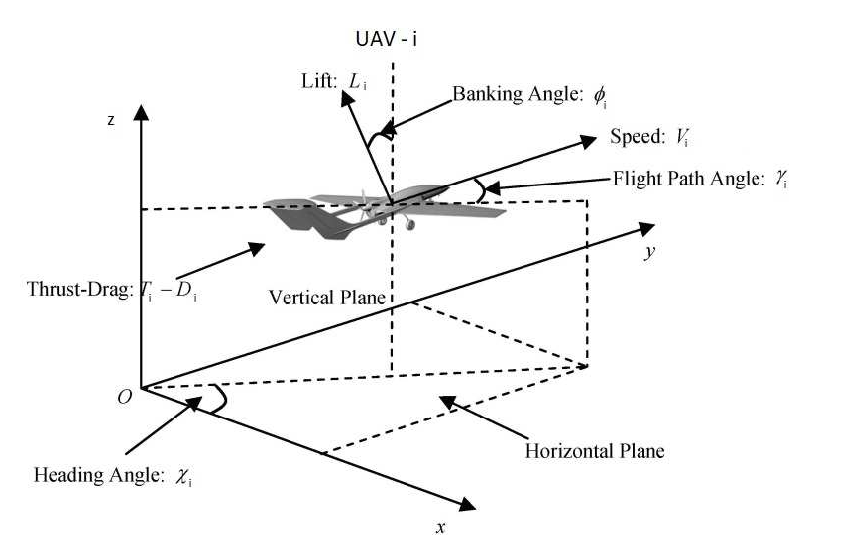
\includegraphics[width=0.8\linewidth]{images/Chapter5/UAV.png}
        \caption{Parameters of $i-$th UAV, \cite{9213862}.}
        \label{fig:5.1}
    \end{figure}
     Let $F_i = [T_i\hspace{3.0mm} L_isin(\phi_i)\hspace{5.0mm}  L_icos(\phi_i)]^T$ be the control input, $p_i = [x_i\hspace{5.0mm}  y_i\hspace{5.0mm}  z_i]^T$ the position vector and $v_i = \dot{p}_i = [\dot{x}_i\hspace{5.0mm}  \dot{y}_i\hspace{5.0mm}  \dot{z}_i]^T$ the velocity vector. Then, from the equations (\ref{eq:5.1.1}), (\ref{eq:5.1.2}) it is derived that
     \begin{equation}\label{eq:5.1.3}
         \begin{align*}
             \dot{p}_i &= \hspace{2.0mm} v_i\\
             m_i \dot{v}_i &= \hspace{2.0mm} \eta_i + m_i \varepsilon_i + G_iF_i
         \end{align*}
     \end{equation}
     where
     \begin{equation}\label{eq:5.1.4}
         \eta_i = \left[\begin{matrix}
             -D_i cos(\chi_i) cos(\gamma_i)\\
             -D_i sin(\chi_i) cos(\gamma_i)\\
             -D_i sin(\gamma_i)
         \end{matrix}\right]
     \end{equation}
     \vspace{2.0mm}
     \begin{equation}\label{eq:5.1.5}
         \varepsilon_i = [0 \hspace{2.0mm} 0 \hspace{2.0mm} g]^T
     \end{equation}
    and
    \begin{equation}\label{eq:5.1.6}
        G_i = \left[\begin{matrix}
            cos(\chi_i) cos(\gamma_i) & -sin(\chi_i) & -sin(\gamma_i) cos(\chi_i)\\
            sin(\chi_i) cos(\gamma_i) & cos(\chi_i) & -sin(\chi_i) cos(\gamma_i)\\
            sin(\gamma_i) & 0 & cos(\gamma_i)
        \end{matrix}\right]
    \end{equation}
    
    \vspace{4.0mm}
    
    It can be seen that $G_i^{-1} = G_i^T$. Every UAV communicate its position through the graph configuration in sampled time periods. Thus, its output is going to be $\boldsymbol{x}_i := \boldsymbol{p}_i$. Every UAV has a local nonconvex cost function $f_i(x_i,y_i,z_i)$ which is unknown. The algorithm \ref{alg:reg-prox-gpda} has a gradient approximation, thus only the information of the gradient is required in order to update the primal and dual variable. Consider that the input of the system is given by $F_i = G_i^T (u_i + d_i)$, with $u_i = [u_{i_x} \hspace{3.0mm} u_{i_y} \hspace{3.0mm} u_{i_z}]^T$ and $d_i = [d_{i_x} \hspace{3.0mm} d_{i_y} \hspace{3.0mm} 0]^T$. Then, the dynamics of every agent will be
    \begin{equation}\label{eq:5.1.7}
        \begin{align*}
             \dot{p}_i &= \hspace{2.0mm} v_i\\
             m_i \dot{v}_i &= \hspace{2.0mm} \eta_i + m_i \varepsilon_i + u_i + d_i\\
             x_i &= \hspace{2.0mm} p_i
         \end{align*}
    \end{equation}
     
\section{System Simulation with MATLAB}

    In this section, the simulations of the proposed algorithm with control scheme will be presented. The system is a network of $N = 5$ UAV agents which have dynamics from (\ref{eq:5.1.7}), and control laws of (\ref{eq:4.2.9}),(\ref{eq:4.2.10}). All the signals of the closed-loop system ought to be bounded, and the error variable tends to zero, as the agents reach the optimal stationary point.
    
\subsection{Parameters of the System}

    Every agent has a local cost function $f_i(x_i,y_i,z_i)$, $i\in \mathcal{V}$. The communication graph of the agents is shown in figure \ref{fig:5.2} . It can be seen that is connected as is perquisite of the assumption A.\ref{asm:4}.

    \begin{figure}[H]
        \centering
        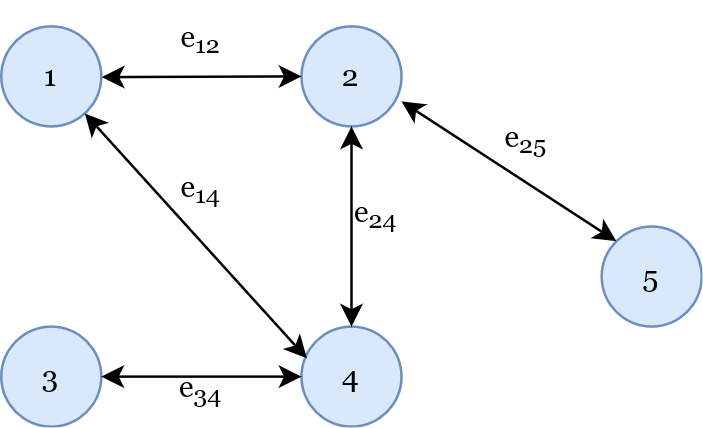
\includegraphics[width=0.5\linewidth]{images/Chapter5/Graph 1.png}
        \caption{Communication Graph of UAVs.}
        \label{fig:5.2}
    \end{figure}
    The incidence matrix of the communication graph of figure \ref{fig:5.2}, based on definition \ref{def:2.9} with its elements computed by equation (\ref{eq:2.1.1}), is
    \begin{equation*}
        \mathcal{A} = \left[\begin{matrix}
            1 & -1 & 0 & 0 & 0\\
            1 & 0 & 0 & -1 & 0\\
            0 & 1 & 0 & -1 & 0\\
            0 & 1 & 0 & 0 & -1\\
            0 & 0 & 1 & -1 & 0
        \end{matrix}\right]
    \end{equation*}

    The Laplacian matrix of the graph will be computed by equation (\ref{eq:2.1.3}), which is also the signed Laplacian. So
    \begin{equation*}
        L = L_- = \mathcal{A}^T\mathcal{A} =\left[\begin{matrix}
            1 & 1 & 0 & 0 & 0\\
            -1 & 0 & 1 & 1 & 0\\
            0 & 0 & 0 & 0 & 1\\
            0 & -1 & -1 & 0 & -1\\
            0 & 0 & 0 & -1 & 0
        \end{matrix}\right] \left[\begin{matrix}
            1 & -1 & 0 & 0 & 0\\
            1 & 0 & 0 & -1 & 0\\
            0 & 1 & 0 & -1 & 0\\
            0 & 1 & 0 & 0 & -1\\
            0 & 0 & 1 & -1 & 0
        \end{matrix}\right] = \left[ \begin{matrix}
            2 & -1 & 0 & -1 & 0\\
            -1 & 3 & 0 & -1 & -1\\
            0 & 0 & 1 & -1 & 0\\
            -1 & -1 & -1 & 3 & 0\\
            0 & -1 & 0 & 0 & 1
        \end{matrix}\right]
    \end{equation*}
    \begin{equation*}
        \Rightarrow L = \left[ \begin{matrix}
            2 & -1 & 0 & -1 & 0\\
            -1 & 3 & 0 & -1 & -1\\
            0 & 0 & 1 & -1 & 0\\
            -1 & -1 & -1 & 3 & 0\\
            0 & -1 & 0 & 0 & 1
        \end{matrix}\right]
    \end{equation*}
    The degree matrix of the graph can be computed from definitions (\ref{def:2.7}) and (\ref{def:2.8}). So,
    \begin{equation*}
        D = diag\{2,3,1,3,1\}
    \end{equation*}
    Finally, the signless Laplacian matrix will be computed from equation (\ref{eq:2.1.4}). So,
    \begin{equation*}
        L_{+} = 2D - \mathcal{A}^T\mathcal{A} = \left[\begin{matrix}
            4 & 0 & 0 & 0 & 0\\
            0 & 6 & 0 & 0 & 0\\
            0 & 0 & 2 & 0 & 0\\
            0 & 0 & 0 & 6 & 0\\
            0 & 0 & 0 & 0 & 2
        \end{matrix}\right] - \left[\begin{matrix}
            2 & -1 & 0 & -1 & 0\\
            -1 & 3 & 0 & -1 & -1\\
            0 & 0 & 1 & -1 & 0\\
            -1 & -1 & -1 & 3 & 0\\
            0 & -1 & 0 & 0 & 1
        \end{matrix}\right] = \left[\begin{matrix}
            2 & 1 & 0 & 1 & 0\\
            1 & 3 & 0 & 1 & 1\\
            0 & 0 & 1 & 1 & 0\\
            1 & 1 & 1 & 3 & 0\\
            0 & 1 & 0 & 0 & 1
        \end{matrix}\right]
    \end{equation*}

    The initial conditions of every $i-$th agent is presented by in the below vectors.
    \begin{equation*}
        \begin{align}
            x(0) &= [1, \hspace{3.0mm} 1.5, \hspace{3.0mm} 4, \hspace{3.0mm} -0.1, \hspace{3.0mm} 3]^T\\
            y(0) &= [0, \hspace{3.0mm} -2, \hspace{3.0mm} 1, \hspace{3.0mm} 5, \hspace{3.0mm} 2.5]^T\\
            z(0) &= [1, \hspace{3.0mm} 2.4, \hspace{3.0mm} 2, \hspace{3.0mm} 0.5, \hspace{3.0mm} 3.4]^T
        \end{align}
    \end{equation*}
    while the masses of the agents are presented in table \ref{tab:5.1}.
    \begin{table}[h]
        \centering
        \begin{tabular}{c c c c c c}
        \hline
            $i$ &  1 & 2 & 3 & 4 & 5\\
            $m_i (kg)$ & 2.1 & 3.2 & 2 & 1.8 & 2.8\\
        \hline
        \end{tabular}
        \caption{Mass of every agent.}
        \label{tab:5.1}
    \end{table}

    The parameters of the system that change in every scenario are presented in table \ref{tab:5.2}.
    \begin{table}[h]
        \centering
        \begin{tabular}{|c||c|}
        \hline
             Parameters &  Description\\
             \hline\hline
             $x_i(0)$,$y_i(0)$,$z_i(0)$ & Initial conditions of every agent\\
             \hline
             $x_{obs}$ & Position of an obstacle\\
             \hline
             $\tau$ & Obstacle distance\\
             \hline
             $S$, $U$ & Cost function constants\\
             \hline
             $D$ & Number of Delay Periods\\
             \hline
             $T$ & Sampled Period Time\\
             \hline
             $d_{max}$ & Communication delay\\
             \hline
             $\beta$ & penalty parameter\\
             \hline
             $c$ & Algorithm candidate function constant\\
             \hline
             $\epsilon$ & Algorithm convergence value\\
             \hline
             $\mathrm{L}$ & Lipschitz constant\\
             \hline
             $\vartheta_i$ & Sliding manifold gain parameters\\
             \hline
             $k_{i_1}$ & Controller gain\\
             \hline
             $\lambda_1$, $\lambda_2$ & Exponential gain parameters\\
        \hline
        \end{tabular}
        \caption{Variables of simulation}
        \label{tab:5.2}
    \end{table}



\subsection{Scenario 1: Optimal Consensus}
    As a first scenario of simulation, the local cost function will have a simple nonconvex form with $f_i(x_i) = \frac{1}{1 + e^{-a_ix_i}}$, with $a_i = \{2.4, 1.3, 0.5, 0.84, 1.25\}$.

















\subsection{Scenario 2: Optimal Consensus with Obstacle Avoidance}

    In the second scenario, the local cost function of every agent will have a different form to avoid a static obstacle. A good nonconvex suitable function for every agent is $f_i(x_i) =  \left \lVert x_i - x_i(0) \right \rVert^2 - \frac{\tau}{\tau + 1}  \left \lVert x_i - x_{obs} \right \rVert^2 $, with $\tau > 0$. With this cost function, the agents will achieve optimal consensus while avoiding a static obstacle with coordinates $x_{obs}$ and maintaining a short distance from the initial point $x_i(0)$ of every agent for reduced energy consumption, \cite{10125000}. The parameter $\tau$ sets the distance of the static obstacle from the agents. If $\tau = 0$ then the obstacle does not exist, while for an enormous value the obstacle has a significant distance from the agents' positions. In this, particular scenario is assumed that the distance parameter has value $\tau = 0.4$ and the coordinates of the obstacle are $x_{obs} = [1.5, \hspace{2.0mm} 2, \hspace{2.0mm} 1.8]^T$. 


















    
\subsection{Scenario 3: Formation Control with Obstacle Avoidance}

    Apart from the optimal consensus problem, agents perform tasks in a formation. This is defined as formation control. In this scenario, the agents must hold a certain a formation, while avoiding a static obstacle with coordinates $x_{obs}$ and maintaining a short distance from the initial point $x_i(0)$ of every agent for reduced energy consumption, \cite{10125000}. This is commonly referred to as the optimal formation control problem, which transforms the formation control problem to an optimal consensus one with variables $\Bar{x}_i := x_i - x_{f_i}$, where $x_{f_i}$ is the vector that indicates the position of every agent $i$ in a specified formation. Let the desired formation be a pentagon, then
    \begin{equation*}
        x_{f_i} = R\left[\begin{matrix}
            cos \left(\frac{\pi}{3}i\right)\\
            sin \left(\frac{\pi}{3}i\right)\\
            z_f
        \end{matrix}\right], i = 1,...,5
    \end{equation*}
    for a radius $R > 0$. So, the new optimal consensus problem for the output variables $\bar{x}_i$ with cost function $g\left(\bar{x}_i\right) = f_i\left(\bar{x}_i + x_{f_i}\right)$ will be
    \begin{equation*}
        g\left(\bar{x}_i\right) = \left\lVert \bar{x}_i + x_{f_i} - x_i(0) \right\rVert^2 - \frac{\tau}{\tau + 1} \left\lVert \bar{x}_i + x_{f_i} - x_{obs} \right\rVert^2
    \end{equation*}
    with $\tau > 0$. Then, the new NOCGPROX variables will have form
    \begin{equation*}
        q_i(t) = \bar{x}_i(t) - \rho \left(t - \left\lfloor \frac{t}{T} \right\rfloor T \right) s_i \left(\left\lfloor \frac{t}{T} \right\rfloor T \right) - \left[1 - \rho\left(t - \left\lfloor \frac{t}{T} \right\rfloor T \right)\right] s_i \left(\left\lfloor \frac{t}{T} \right\rfloor T - T \right)
    \end{equation*}
    where the discrete time vector $s_i$ is defined as
    \begin{equation*}
        \begin{align}
            s_i\left(\left\lfloor \frac{t}{T} \right\rfloor T \right) = \bar{x}_i\left(\left\lfloor \frac{t}{T} \right\rfloor T \right) - \frac{1}{2\beta d_i}&\left[\beta \sum_{j \in \mathcal{N}(i)} \bar{x}_j\left(\left\lfloor \frac{t}{T} \right\rfloor T \right) - \nabla g_i \left( \bar{x}_i\left(\left\lfloor \frac{t}{T} \right\rfloor T \right)\right)\right\\ 
            &\left -\beta \sum_{j \in \mathcal{N}(i)} \sum_{\ell = 1}^{\lfloor t/DT \rfloor} \left(\bar{x}_i\left( \ell \left\lfloor \frac{t}{T} \right\rfloor T \right) - \bar{x}_j\left( \ell \left\lfloor \frac{t}{T} \right\rfloor T \right)\right) \right]
        \end{align}
    \end{equation*}
    for every agent $i \in \mathcal{V}$, with $\beta > 0$. The control laws have the same form and guarantee that that error variables tend to zero and are square integrable. Therefore, the swarm will achieve the desired formation.



    
    
 
%--------------------------------------------------------------------   
    
    \chapter{Epilogue}
    \section{Conclusions}

    The aim of this thesis was to solve the proximal optimal consensus problem for a class of nonlinear agents with non-convex cost functions and constraints. In order to achieve consensus, a regulation form of Prox-GPDA, \cite{pmlr-v70-hong17a}, was designed with the addition of the NOn-Convex Gradient PROXimal (NOCGPROX) variables. These variables use sampled output measurements of the agents in a continuous manner to transform the optimal consensus problem into a regulation problem. In addition, robust distributed control laws were designed in order to achieve optimal consensus between the agents. The control laws were designed with a sliding mode backstepping approach with the use of Nussbaum gains. The crucial element for the applicability of this algorithm was the guarantee of the quadratic integration of the suggested variables. This approach enabled the algorithm to achieve sublinear convergence with a small number of iterations, while all signals of the closed-loop system proved to be bounded, attaining asymptotic stability. As a result, for the first time was proved that during the information exchange between the agents, needed only a finite amount of energy while transmitting the output sampled measurements. Therefore, the UAVs achieve optimal consensus with the proposed distributed control laws and algorithm.

\newpage
\section{Future Work}

    The proposed methodology that was researched in this thesis assumes that the output measurements are known. In certain application, sensors can not measure the output of a system. Thus, it is difficult to apply the above proposition. A sufficient solution to this problem is to seek Nash or Stackelberg equillibriums. This method does not require the knowledge of the output, hence it is estimated from the use of dynamic games. Another extension to this thesis is the use of switching topology. In that case, new robust distributed laws need to be applied to ensure that the switching of the topology does not have an impact in the communications between the agents. Therefore, consensus will be achieved. Another extension to the problem is the use of Control Barrier Functions to ensure a safe environment for the agents in the presence of obstacles. The inclusion of these constraints will create reliable planning for the agents to achieve optimal consensus regarding the position of these obstacles. Additionally, another area that this methodology can be tested is in networks with malicious agents. Due to the fact that the information exchange between the agents is occurring in lower band frequencies with a certain delay factor, the network can be expanded with these agents to increase the security of the network. As a result, new distributed control laws will be developed to guarantee the secure exchange of information between the agents. 
 
%--------------------------------------------------------------------    
    \cleardoublepage
    \phantomsection
    \addcontentsline{toc}{chapter}{Bibliography}
    \nocite{*}
    \printbibliography

\end{document} 